\documentclass[a4paper,latin]{paper}
\setcounter{secnumdepth}{5}
\setcounter{tocdepth}{5}
\usepackage[english]{babel}  
\usepackage[margin=2cm]{geometry}
\usepackage{graphicx}
\usepackage{lipsum}
\usepackage{xcolor}
\usepackage{booktabs}
\usepackage{listings}
\usepackage{hyperref}
\hypersetup{pdftex,colorlinks=true,allcolors=black}
\usepackage{hypcap}
\usepackage[toc,acronym]{glossaries}
\usepackage{tikz}
\usetikzlibrary{automata,positioning,calc,tikzmark,decorations.pathreplacing}
\usepackage{tabularx,colortbl}
\usepackage{fancyhdr}
\usepackage{extramarks}
\usepackage{framed}
\usepackage{calc}
\usepackage{textcomp}

% redefine subparagraph, do not indent
\makeatletter
\renewcommand\subparagraph{\@startsection{subparagraph}{5}{\z@}%
                                     {-3.25ex\@plus -1ex \@minus -.2ex}%
                                     {-5pt \@plus .2ex}%
                                     {\normalfont\normalsize\bfseries}}
\makeatother

\lstdefinestyle{BashInputStyle}{
  language=bash,
  basicstyle=\small\ttfamily,
  numberstyle=\tiny,
  numbersep=3pt,
  frame=tb,
  columns=fullflexible,
  keepspaces=true,
  showstringspaces=false,
  backgroundcolor=\color{yellow!20},
  linewidth=1\linewidth,
  breaklines=true,
  upquote=true,
  postbreak=\raisebox{0ex}[0ex][0ex]{\ensuremath{\color{red}\hookrightarrow\space}},
  xleftmargin=0.0\linewidth
}
\lstdefinestyle{LuaInputStyle}{
  language={[5.1]Lua},
  basicstyle=\small\upshape\ttfamily,
  numberstyle=\tiny,
  numbersep=3pt,
  keywordstyle=\color{blue}\bfseries,
  stringstyle=\color{magenta},
  frame=tb,
  columns=fullflexible,
  keepspaces=true,
  showstringspaces=false,
  backgroundcolor=\color{orange!30},
  linewidth=1\linewidth,
  breaklines=true,
  upquote=true,
  postbreak=\raisebox{0ex}[0ex][0ex]{\ensuremath{\color{red}\hookrightarrow\space}},
  xleftmargin=0.0\linewidth,
  morekeywords={vpget, vpset, vpval, vpsize, vpnew, getval},
  otherkeywords={.}
}

\sectionfont{\large\sf\bfseries\color{black!70!blue}} 
\renewcommand\keywordname{Clavem verborum}
\title{Release14 SMS Filtering}
\subtitle{Configuration and maintenance\\
\hfill
\includegraphics[height=2cm]{graphics/octopus.jpg}
\vspace{-1cm}}
\def\findrootlanguage{%
   \def\rootlanguagename{english}%
}

\makeglossaries
\newglossaryentry{node}
{
  name=node,
  description={A node is a running instance of pMINK daemon, usually belonging to a cluster}
}
\newglossaryentry{cluster}
{
  name=cluster,
  description={A cluster consists of one or more nodes which share the same pMINK daemon type}
}
\newglossaryentry{daemon}
{
  name=daemon,
  description={Daemon is a computer program that runs as a background process, rather than being under the direct control of an interactive user}
}
\newglossaryentry{routing}
{
  name=routing,
  description={In internetworking, the process of moving a packet of data from source to destination. Routing is usually performed by a dedicated device called a router}
}
\newglossaryentry{threat}
{
  name=threat,
  description={A circumstance or event that has or indicates the potential to exploit vulnerabilities and to adversely impact (create adverse consequences for) 
	       organizational operations, organizational assets (including information and information systems), individuals, other organizations, or society}
}
\newglossaryentry{rule}
{
  name=rule,
  description={A piece of system logic that is evaluated by \acrfull{rpe}} 
}
\newglossaryentry{bcintr}
{
  name=bytecode interpreter,
  description={A virtual machine, or bytecode interpreter, is a sort of simulation of a computer, usually used to implement a script language. You define an 
	       instruction set for this machine according to the needs of your script language. The instructions for the virtual computer are called "bytecodes"} 
}
\newglossaryentry{bytecode}
{
  name=bytecode,
  description={Bytecode is computer object code that is processed by a program, usually referred to as a virtual machine, rather than by the "real" computer machine, 
	       the hardware processor}
}
\newglossaryentry{x690}
{
  name=X.690,
  description={X.690 is an ITU-T standard specifying several ASN.1 encoding formats: Basic Encoding Rules (BER), Canonical Encoding Rules (CER) and
    	       Distinguished Encoding Rules (DER)}
}
\newglossaryentry{asn1}
{
  name=ASN.1,
  description={Abstract Syntax Notation One (ASN.1) is a standard and notation that describes rules and structures for representing, encoding, transmitting, and 
	       decoding data in telecommunications and computer networking}
}
\newglossaryentry{perl}
{
  name=perl,
  description={Perl is a family of high-level, general-purpose, interpreted, dynamic programming languages. The languages in this family include Perl 5 and Perl 6}
}

\newglossaryentry{boolean}
{
  name=boolean,
  description={In computer science, a Boolean expression is an expression in a programming language that produces a Boolean value when evaluated, i.e. one of true or false. 
	       A Boolean expression may be composed of a combination of the Boolean constants true or false, Boolean-typed variables, Boolean-valued operators, and Boolean-valued functions}
}
\newglossaryentry{zbased}
{
  name=zero-based,
  description={Zero-based numbering or index origin = 0 is a way of numbering in which the initial element of a sequence is assigned the index 0, rather than the index 1 as 
	       is typical in everyday non-programming circumstances}
}
\newglossaryentry{regex}
{
  name=regular expression,
  description={In theoretical computer science and formal language theory, a regular expression (sometimes called a rational expression) is a sequence of characters that define 
	       a search pattern, mainly for use in pattern matching with strings, or string matching, i.e. "find and replace"-like operations}
}
\newglossaryentry{lua}
{
  name=lua,
  description={Lua is a lightweight multi-paradigm programming language designed primarily for embedded systems and clients. Lua is cross-platform since it is written in ANSI C, 
	       and has a relatively simple C API}
}
\newglossaryentry{variant}
{
  name=variant,
  description={A Variant is a special data type that can contain any kind of data}
}





\newacronym{fgn}{FGN}{Filtering Gateway Node}
\newacronym{sgn}{SGN}{Signalling Gateway Node}
\newacronym{stp}{STP}{Signalling Transfer Point}
\newacronym{pmink}{pMINK}{Project MINK Framework}
\newacronym{r14p}{R14P}{Release14 Application Layer Protocol}
\newacronym{rrp}{RRP}{Release14 Routing and Rating Protocol}
\newacronym{routingd}{ROUTINGD}{R14P Routing Daemon}
\newacronym{configd}{CONFIGD}{pMINK Configuration Daemon}
\newacronym{cli}{CLI}{pMINK Command Line Interface}
\newacronym{sms}{SMS}{Short Message Service}
\newacronym{cdr}{CDR}{Call Data Record}
\newacronym{wrr}{WRR}{Weighted Round Robin}
\newacronym{fsm}{FSM}{Finite-state machine}
\newacronym{rpe}{RPE}{Rule Processing Engine}
\newacronym{rproc}{RPROC}{Rule Processor}
\newacronym{rel}{REL}{Rule Execution Logic}
\newacronym{smstpdu}{SMSTPDU}{Short message TPDU 3GPP TS 23.040}
\newacronym{tp-oa}{TP-OA}{TP-Originating-Address}
\newacronym{tp-da}{TP-DA}{TP-Destination-Address}
\newacronym{ton}{TON}{Type Of Number}
\newacronym{nai}{NAI}{Nature Of Address Indicator}
\newacronym{np}{NP}{Numbering Plan}
\newacronym{m3ua}{M3UA}{MTP Level 3 (MTP3) User Adaptation Layer}
\newacronym{sccp}{SCCP}{Signalling Connection Control Part}
\newacronym{tcap}{TCAP}{Transaction Capabilities Application Part}
\newacronym{map}{MAP}{Mobile Application Part}
\newacronym{smpp}{SMPP}{Short Message Peer-to-Peer}
\newacronym{tcp}{TCP}{Transmission Control Protocol}
\newacronym{sctp}{SCTP}{Stream Control Transmission Protocol}
\newacronym{as}{AS}{Application Server}
\newacronym{asp}{ASP}{Application Server Process}
\newacronym{lci}{LCI}{Left Component Index}
\newacronym{rci}{RCI}{Right Component Index}
\newacronym{pdu}{PDU}{Protocol Data Unit}
\newacronym{api}{API}{Application Programming Interface}
\glsaddall

\begin{document} 
\pagenumbering{arabic}
\pagestyle{fancy}
\onecolumn\maketitle 
\hrule 
\tableofcontents
\hrule\bigskip
\clearpage
\section{Legal notices}

This document, or any part thereof, may not, without the written consent of Release 14 LTD,
be copied, reprinted or reproduced in any material form including but not limited to
photocopying, transcribing, transmitting or storing it in any medium or translating it into any
language, in any form or by any means, be it electronic, mechanical, optical, magnetic or
otherwise.

The information contained herein is believed to be accurate and reliable. Release14 LTD
accepts no responsibility for its use by any means or in any way whatsoever. Release14 LTD
shall not be liable for any expenses, costs or damage that may result from the use of the
information contained within this document. The information contained herein is subject to
change without notice.

\section{Introduction}

This document describes various configuration options for the R14 SMS Filtering software.

\subsection{Intended audience}

This guide is intended for experienced network and system administrators who are familiar with
using command line interface languages.

\subsection{Document conventions}

This document uses the following typographic conventions.

\begin{tabular}{ l l }
Monospace & - examples, command line output \\
\textbf{Bold Monospace} & - what you type at the command line \\
\textbf{Bold} & - commands, keywords and file names \\
\textit{Italics} & - variables and values \\
\textless{}key\textgreater & - A key on your keyboard, such as \textless{}Space\textgreater, \\
& - Combinations of keys are joined with a "+" sign
\end{tabular}

\section{Using the CLI}

This chapter provides an overview of the SMS Filtering command line interface which is the
primary interface for SMS Filtering software.

\subsection{Command modes}

There are two operational modes in SMS Filtering, operational and configuration mode. In the
current version operational mode is used solely for accessing the configuration mode. When
you log into the system you are in operational mode.
Configuration mode provides access to commands for creating, modifying, deleting,
committing and showing configuration information, as well as commands for navigating
through the configuration hierarchy.

\begin{itemize}
	\item To enter configuration mode from operational mode issue \textbf{configure} command
	\item To return to the operational mode press \textless{}Ctrl\textgreater{}+d. If there are uncommitted
	      configuration changes they will be discarded after a timeout? Pressing \textless{}Ctrl\textgreater{}+d again
	      in operational mode will log you out of the system.
\end{itemize}

\subsection{Accessing the CLI}

To access the command line interface of R14 SMS Filtering software you connect with SSH on port 22
with a predefined username and password.

\subsection{Predefined user account}

By default, currently the system has one predefined user account, the user \textbf{config}. The default
password for user config is \textbf{config}. The \textbf{config} user has administrator level privileges and can execute
all SMS Filtering commands

\subsection{Command prompts}

The command prompt shows the user account you are logged in, the hostname of the system and
whether you are in operational mode or configuration mode.\newline\newline
The format of command prompt in operational mode is as follows
\begin{lstlisting}[style=BashInputStyle]
config@hostname:/ >
\end{lstlisting}
The format of command prompt in configuration mode is as follows:
\begin{lstlisting}[style=BashInputStyle]
config@hostname:/configure >
\end{lstlisting}

\subsection{Command completion}

SMS Filtering software can auto complete command syntax by entering the following:\newline

\begin{tabular}{ l | p{0.4\textwidth} }
	\textless{}Tab\textgreater & Auto-completes a command \\
				   & \begin{itemize} 
        				\item If the command is unambiguous the system generates the next token in the syntax 
					\item If more than one completion is possible the system displays a set of next possible tokens
				     \end{itemize} \\
	? followed by	           &  Pressing the \textless{}Tab\textgreater{}key after question mark generates context aware command completion assistance \\
	\textless{}Tab\textgreater &  command completion assistance \\
	\textless{}Tab\textgreater &  Displays all available SMS Filtering commands
\end{tabular}

\subsection{Command history}

The SMS Filtering command line interface supports a command history, where commands you
executed are stored in a internal buffer and can be re-executed or edited.\newline

\begin{tabular}{ l l }
	\textless{}Up-Arrow\textgreater   & Move to the previous command \\
	\textless{}Down-Arrow\textgreater & Move to the next command
\end{tabular}

\subsection{Command editing}

The SMS Filtering command line interface supports command editing\newline

\begin{tabular}{ l l }
	\textless{}Right-Arrow\textgreater   & Move forward in the command line \\
	\textless{}Left-Arrow\textgreater    & Move backward in the command line
\end{tabular}

\subsection{Command timeout}

SMS Filtering command line interface has a timeout of 60 seconds. If there is no activity on the
system in that time frame, configuration changes that haven’t been committed will be lost.

\section{Configuration basics}

\subsection{Terminology}

Several versions of system configuration exist:
\begin{itemize}
	\item \textbf{Active or running configuration.} This is the configuration that is actually loaded and
	      used by the system.
	\item \textbf{Working configuration.} When you enter configuration mode and make changes,
	      changes remain in working configuration until you commit the changes, at which
	      time the configuration becomes active or running.
	\item \textbf{Saved configuration.} If you save configuration with the \textbf{save} command to a file.
\end{itemize}

\subsection{Configuration hierarchy}

SMS Filtering configuration is organized as a hierarchy of configuration statements with a
hierarchical tree of nodes similar to the directory structure on a UNIX file system. There are
three kinds of statements:
\begin{itemize}
	\item Configuration nodes. This can be either:
		\begin{enumerate}
			\item Single nodes
			\item Multi-nodes
			\item Attribute statements. These set the values or characteristics for parameters within a node.
		\end{enumerate}
\end{itemize}
From the system’s point of view, a configuration node is different from a simple
configuration attribute statement. A configuration \textit{attribute statement} takes the form
\textit{attribute value}, as in the following example.
\begin{lstlisting}[style=BashInputStyle]
priority    100
\end{lstlisting}
A configuration \textit{node} always has an enclosing pair of braces as in the following example:
\begin{lstlisting}[style=BashInputStyle]
rule_1 {
    priority "100"
}
\end{lstlisting}

\subsection{Entering and exiting configuration mode}

\begin{itemize}
	\item To enter configuration mode from operational mode issue \textbf{configure} command.
		\begin{lstlisting}[style=BashInputStyle]
config@hostname:/ > configure
Trying '127.0.0.1:10000'...OK
config@hostname:/configure >
		\end{lstlisting}
	\item To return to the operational mode press \textless{}Ctrl\textgreater+d
	\item To disconnect and exit press \textless{}Ctrl\textgreater+d
\end{itemize}

\subsection{Navigating in configuration mode}

You can tell where you are in the configuration tree by the path in tree:
\begin{lstlisting}[style=BashInputStyle]
config@hostname:/configure/mno/fgn/fgn1 >
\end{lstlisting}

\subsection{Commands for navigating in configuration mode}

\begin{tabular}{ | l | l | }
	\hline
	Command 			& Result \\ \hline
	\textbf{edit config-node}	& Navigates to a subnode in the configuration tree for editing \\
	\textbf{top}			& Exits to the top level of configuration mode \\
	\textbf{up}			& Navigates up one level in the configuration tree \\
	\hline
	
\end{tabular}

\subsection{Viewing the configuration}

Use the show command in configuration mode to display node configuration:
\begin{lstlisting}[style=BashInputStyle]
config@hostname:/configure > show mno fgn fgn1 
        pool [   10000 ] - Correlation and rule processor pool size
     timeout [       5 ] - Default correlation timeout             
   timer_res             - Timer resolution in seconds
    fworkers [       4 ] - Number of rule processor threads
 sl_list_max [ 1000000 ] - Maximum number of elements in standard list (default = 1000)
 fl_list_max             - Maximum number of elements in flood list (default = 1000)
 fl_list_ttl             - Maximum flood list TTL in seconds (default = 3600)
     routing             - Routing nodeset configuration                     
      rating             - Rating nodeset configuration 
       lists             - Filtering lists             
       rules             - Filter configuration
\end{lstlisting}
Use the \textbf{configuration} command to display the whole SMS Filtering configuration

\begin{lstlisting}[style=BashInputStyle]
config@hostname:/configure > configuration
mno {
  fgn {
    fgn1 {
      pool        "10000"
      timeout     "5"
      fworkers    "4"
      sl_list_max "1000000"
      rating {
        rating-01 {
          remote {
            address "192.168.0.20"
            port    "33000"
          }
          local {
            address "192.168.0.10"
            port    "34001"
          }
          weight "1"
        }
      }
      rules {
        test-rule-00000 {
          description   "--- Block Alphasenders ---"
	  priority      "10000"
          filter_result "2"
          definition {
            match {
              r14p {
                trunk_label "[+]TEST_T01_IN"
              }
              map {
                context {
                  sm {
                    imsi ":24412.*"
                  }
                }
              }
              smstpdu {
                tp-oa {
                  ton     "80"
                }
              }
            }
            translate {
              filter_result "2"
              filter_jump   "_lvl3-sms-originating-alphasender-blocked_10100000"
            }
          }
        }
        _lvl3-sms-originating-alphasender-blocked_10100000 {
          description   "--- Block Alphasender --- Level 3 ---"
          priority      "10100000"
          filter_result "0"
          definition {
            translate {
              filter_result "0"
            }
          }
        }
      }
    }
  }
}

\end{lstlisting}

\section{Changing configuration information}

\subsection{Adding or modifying configuration}

Add new configuration by creating a configuration node, using the \textbf{set} command in
configuration mode. Modify existing configuration using the \textbf{set} command in configuration
mode, as in the following example:
\begin{lstlisting}[style=BashInputStyle]
config@hostname:/configure > set mno fgn fgn1 rules test-rule-00000 description "test text"
config@hostname:/configure 
\end{lstlisting}
Then us the \textbf{show} command to see the change:
\begin{lstlisting}[style=BashInputStyle]
config@hostname:/configure > show mno fgn fgn1 rules test-rule-00000
   +description [ test text ] - Rule description
       priority [     10000 ] - Priority level  
  filter_result [         2 ] - Default filtering result
     definition               - Rule configuration
\end{lstlisting}
Note the "+" in front of the new statement. This shows that this statement has been added
to the configuration but the change is not yet committed. The change does not take effect
until configuration is committed using the \textbf{commit} command.\newline\newline
The "+" is also visible while using the \textbf{configuration} command:
\begin{lstlisting}[style=BashInputStyle]
test-rule-00000 {
  +description  "test text"
  priority      "10000"
  filter_result "2"
  definition {
    match {
      r14p {
        trunk_label "[+]TEST_T01_IN"
      }
      map {
        context {
          sm {
            imsi ":24412.*"
          }
        }
      }
      smstpdu {
        tp-oa {
          ton     "80"
        }
      }
    }
    translate {
      filter_result "2"
      filter_jump   "_lvl3-sms-originating-alphasender-blocked_10100000"
    }
  }
} 
\end{lstlisting}
You can modify configuration from the root of the configuration tree or use the \textbf{edit}
command to navigate to the part of the tree where you want to change or add.

\subsection{Deleting configuration}

Use the \textbf{delete} command to delete a value, as in the following example:
\begin{lstlisting}[style=BashInputStyle]
config@hostname:/configure > delete mno fgn fgn1 rules test-rule-00000 description
\end{lstlisting}
You can use the \textbf{show} command to see the change:
\begin{lstlisting}[style=BashInputStyle]
config@hostname:/configure > show mno fgn fgn1 rules test-rule-00000
   -description [ test text ] - Rule description
       priority [     10000 ] - Priority level  
  filter_result [         2 ] - Default filtering result
     definition               - Rule configuration
\end{lstlisting}
Note the "-" in front of the deleted statement. This shows that this statement has been
deleted from the configuration but the change is not yet committed. The change does not
take effect until configuration is committed using the \textbf{commit} command.\newline\newline
Use the \textbf{delete} command to delete a complete configuration node, as in the following
example:
\begin{lstlisting}[style=BashInputStyle]
config@hostname:/configure > delete mno fgn fgn1 rules test-rule-00000
\end{lstlisting}
You can use the \textbf{show} command to see the change:
\begin{lstlisting}[style=BashInputStyle]
config@hostname:/configure > show mno fgn fgn1 rules
-test-rule-00000
\end{lstlisting}
Note the "-" in front of the deleted statement. This shows that this statement has been
deleted from the configuration but the change is not yet committed. The change does not
take effect until configuration is committed using the \textbf{commit} command.

\subsection{Committing configuration changes}

In the SMS Filtering software, configuration changes do not take effect until you commit them with
the \textbf{commit} command:
\begin{lstlisting}[style=BashInputStyle]
config@hostname:/configure > commit
\end{lstlisting}
Lines with uncommitted changes are flagged as follows:
\begin{itemize}
	\item "+" to indicate the line has been added
	\item "-" to indicate the line has been removed
\end{itemize}
Once you commit the changes, the flag disappears.

\subsection{Discarding configuration changes}

If you don’t want to commit the changes, you can discard them with the discard command:
\begin{lstlisting}[style=BashInputStyle]
config@hostname:/configure > discard
\end{lstlisting}

\section{Managing system configuration}

\subsection{Saving the running configuration}
Save the running configuration by running the \textbf{save} command in configuration mode. You
must specify the file name and path to the save file location:
\begin{lstlisting}[style=BashInputStyle]
config@hostname:/configure > save file-name /tmp/testconfig.cfg
Saving configuration to "/tmp/testconfig.cfg"...
Done
\end{lstlisting}
You can also save a configuration file to a location path other than the standard
configuration directory by specifying a different path. You can save to a hard drive, compact
Flash, or USB device. Note that the \textbf{save} command writes only committed changes.

\subsection{Loading the saved configuration}

To load a previously saved configuration use the \textbf{load} command in configuration mode. You
must specify the file name and path to the save file location:
\begin{lstlisting}[style=BashInputStyle]
config@hostname:/configure > load file-name /tmp/testconfig.cfg
Loading new configuration file "/tmp/testconfig.cfg"...
Done
Merging new configuration file...
Done
\end{lstlisting}

\subsection{Archiving configuration versions on commit}

The system automatically archives the configuration whenever you commit a configuration
change. By default system maintains unlimited versions of configuration in the archive.

\subsection{Rolling back to previous version}

You can roll back system configuration to any archived version using the \textbf{rollback} command.
\begin{lstlisting}[style=BashInputStyle]
config@hostname:/configure > rollback revision 1
Loading rollback configuration...
Done
Merging rollback configuration file...
Done
Committing rollback configuration...
Done
\end{lstlisting}
The latest commited configuration is revision 0. You can see the list of revisions by using the
context aware completion assistance:
\begin{lstlisting}[style=BashInputStyle]
config@hostname:/configure > rollback revision ?<Tab>
0 - 2013-05-18 10:47:59
1 - 2013-05-18 10:45:11
2 - 2013-05-18 10:44:52
3 - 2013-05-18 10:44:24
4 - 2013-05-18 10:43:24
5 - 2013-05-17 17:50:48
6 - 2013-05-17 17:50:19
7 - 2013-05-17 17:37:43
8 - 2013-05-17 17:37:43
9 - 2013-05-17 17:37:43
\end{lstlisting}

\subsection{Show configuration commands}

You can show all configuration commands for the current configuration by using the
\textbf{commands} command:
\begin{lstlisting}[style=BashInputStyle]
set !pmink
set pmink !routing
set !openli
set openli !leac
set openli leac !db
set openli !dr
set openli !drnfl9
set openli !mediations
set openli !probes
set !mno
set mno !dr
set mno !psgn
set mno !sgn
set mno !fgn
set mno fgn !fg1n
set mno fgn fg1n pool "10000"
set mno fgn fg1n timeout "5"
set mno fgn fg1n fworkers "4"
set mno fgn fg1n sl_list_max "1000000"
set mno fgn fg1n !routing
set mno fgn fg1n !rating
set mno fgn fg1n rating !rating-01
set mno fgn fg1n rating rating-01 !remote
set mno fgn fg1n rating rating-01 remote address "192.168.0.20"
set mno fgn fg1n rating rating-01 remote port "33000"
set mno fgn fg1n rating rating-01 !local
set mno fgn fg1n rating rating-01 local address "192.168.0.10"
set mno fgn fg1n rating rating-01 local port "34001"
set mno fgn fg1n rating rating-01 weight "1"
set mno fgn fg1n !lists
set mno fgn fg1n !rules
set mno fgn fg1n rules !test-rule-00000
set mno fgn fg1n rules test-rule-00000 description "--- Block Alphasenders ---"
set mno fgn fg1n rules test-rule-00000 priority "10000"
set mno fgn fg1n rules test-rule-00000 filter_result "2"
set mno fgn fg1n rules test-rule-00000 !definition
set mno fgn fg1n rules test-rule-00000 definition !match
set mno fgn fg1n rules test-rule-00000 definition match !commands
set mno fgn fg1n rules test-rule-00000 definition match commands !sri-for-sm
set mno fgn fg1n rules test-rule-00000 definition match commands sri-for-sm !cgpa
set mno fgn fg1n rules test-rule-00000 definition match commands sri-for-sm cgpa !gt
set mno fgn fg1n rules test-rule-00000 definition match commands sri-for-sm !cdpa
set mno fgn fg1n rules test-rule-00000 definition match commands sri-for-sm cdpa !gt
set mno fgn fg1n rules test-rule-00000 definition match commands sri-for-sm !nnn
set mno fgn fg1n rules test-rule-00000 definition match commands sri-for-sm !an
set mno fgn fg1n rules test-rule-00000 definition match commands sri-for-sm !msisdn
set mno fgn fg1n rules test-rule-00000 definition match commands sri-for-sm !sca
set mno fgn fg1n rules test-rule-00000 definition match !r14p
set mno fgn fg1n rules test-rule-00000 definition match r14p trunk_label "[+]TEST_T01_IN"
set mno fgn fg1n rules test-rule-00000 definition match !m3ua
set mno fgn fg1n rules test-rule-00000 definition match !sccp
set mno fgn fg1n rules test-rule-00000 definition match sccp !cgpa
set mno fgn fg1n rules test-rule-00000 definition match sccp cgpa !gt
set mno fgn fg1n rules test-rule-00000 definition match sccp !cdpa
set mno fgn fg1n rules test-rule-00000 definition match sccp cdpa !gt
set mno fgn fg1n rules test-rule-00000 definition match !tcap
set mno fgn fg1n rules test-rule-00000 definition match !map
set mno fgn fg1n rules test-rule-00000 definition match map !context
set mno fgn fg1n rules test-rule-00000 definition match map context !sri-for-sm
set mno fgn fg1n rules test-rule-00000 definition match map context sri-for-sm !msisdn
set mno fgn fg1n rules test-rule-00000 definition match map context sri-for-sm !sca
set mno fgn fg1n rules test-rule-00000 definition match map context sri-for-sm !nnn
set mno fgn fg1n rules test-rule-00000 definition match map context sri-for-sm !an
set mno fgn fg1n rules test-rule-00000 definition match map context !sm
set mno fgn fg1n rules test-rule-00000 definition match map context sm imsi ":24412.*"
set mno fgn fg1n rules test-rule-00000 definition match map context sm !scda
set mno fgn fg1n rules test-rule-00000 definition match map context sm !scoa
set mno fgn fg1n rules test-rule-00000 definition match map context sm !msisdn
set mno fgn fg1n rules test-rule-00000 definition match !smstpdu
set mno fgn fg1n rules test-rule-00000 definition match smstpdu !tp-da
set mno fgn fg1n rules test-rule-00000 definition match smstpdu !tp-oa
set mno fgn fg1n rules test-rule-00000 definition match smstpdu tp-oa ton "80"
set mno fgn fg1n rules test-rule-00000 definition match !smpp
set mno fgn fg1n rules test-rule-00000 definition !translate
set mno fgn fg1n rules test-rule-00000 definition translate filter_result "2"
set mno fgn fg1n rules test-rule-00000 definition translate filter_jump "_lvl3-sms-originating-alphasender-blocked_10100000"
set mno fgn fg1n rules test-rule-00000 definition translate !commands
set mno fgn fg1n rules test-rule-00000 definition translate commands !sri-for-sm
set mno fgn fg1n rules test-rule-00000 definition translate commands sri-for-sm !map
set mno fgn fg1n rules test-rule-00000 definition translate commands sri-for-sm !cgpa
set mno fgn fg1n rules test-rule-00000 definition translate commands sri-for-sm cgpa !gt
set mno fgn fg1n rules test-rule-00000 definition translate commands sri-for-sm !cdpa
set mno fgn fg1n rules test-rule-00000 definition translate commands sri-for-sm cdpa !gt
set mno fgn fg1n rules test-rule-00000 definition translate commands sri-for-sm !msisdn
set mno fgn fg1n rules test-rule-00000 definition translate commands sri-for-sm !sca
set mno fgn fg1n rules test-rule-00000 definition translate !r14p
set mno fgn fg1n rules test-rule-00000 definition translate !m3ua
set mno fgn fg1n rules test-rule-00000 definition translate !sccp
set mno fgn fg1n rules test-rule-00000 definition translate sccp !cgpa
set mno fgn fg1n rules test-rule-00000 definition translate sccp cgpa !gt
set mno fgn fg1n rules test-rule-00000 definition translate sccp !cdpa
set mno fgn fg1n rules test-rule-00000 definition translate sccp cdpa !gt
set mno fgn fg1n rules !_lvl3-sms-originating-alphasender-blocked_10100000
set mno fgn fg1n rules _lvl3-sms-originating-alphasender-blocked_10100000 description "--- Block Alphasender --- Level 3 ---"
set mno fgn fg1n rules _lvl3-sms-originating-alphasender-blocked_10100000 priority "10100000"
set mno fgn fg1n rules _lvl3-sms-originating-alphasender-blocked_10100000 filter_result "0"
set mno fgn fg1n rules _lvl3-sms-originating-alphasender-blocked_10100000 !definition
set mno fgn fg1n rules _lvl3-sms-originating-alphasender-blocked_10100000 definition !match
set mno fgn fg1n rules _lvl3-sms-originating-alphasender-blocked_10100000 definition match !commands
set mno fgn fg1n rules _lvl3-sms-originating-alphasender-blocked_10100000 definition match commands !sri-for-sm
set mno fgn fg1n rules _lvl3-sms-originating-alphasender-blocked_10100000 definition match commands sri-for-sm !cgpa
set mno fgn fg1n rules _lvl3-sms-originating-alphasender-blocked_10100000 definition match commands sri-for-sm cgpa !gt
set mno fgn fg1n rules _lvl3-sms-originating-alphasender-blocked_10100000 definition match commands sri-for-sm !cdpa
set mno fgn fg1n rules _lvl3-sms-originating-alphasender-blocked_10100000 definition match commands sri-for-sm cdpa !gt
set mno fgn fg1n rules _lvl3-sms-originating-alphasender-blocked_10100000 definition match commands sri-for-sm !nnn
set mno fgn fg1n rules _lvl3-sms-originating-alphasender-blocked_10100000 definition match commands sri-for-sm !an
set mno fgn fg1n rules _lvl3-sms-originating-alphasender-blocked_10100000 definition match commands sri-for-sm !msisdn
set mno fgn fg1n rules _lvl3-sms-originating-alphasender-blocked_10100000 definition match commands sri-for-sm !sca
set mno fgn fg1n rules _lvl3-sms-originating-alphasender-blocked_10100000 definition match !r14p
set mno fgn fg1n rules _lvl3-sms-originating-alphasender-blocked_10100000 definition match !m3ua
set mno fgn fg1n rules _lvl3-sms-originating-alphasender-blocked_10100000 definition match !sccp
set mno fgn fg1n rules _lvl3-sms-originating-alphasender-blocked_10100000 definition match sccp !cgpa
set mno fgn fg1n rules _lvl3-sms-originating-alphasender-blocked_10100000 definition match sccp cgpa !gt
set mno fgn fg1n rules _lvl3-sms-originating-alphasender-blocked_10100000 definition match sccp !cdpa
set mno fgn fg1n rules _lvl3-sms-originating-alphasender-blocked_10100000 definition match sccp cdpa !gt
set mno fgn fg1n rules _lvl3-sms-originating-alphasender-blocked_10100000 definition match !tcap
set mno fgn fg1n rules _lvl3-sms-originating-alphasender-blocked_10100000 definition match !map
set mno fgn fg1n rules _lvl3-sms-originating-alphasender-blocked_10100000 definition match map !context
set mno fgn fg1n rules _lvl3-sms-originating-alphasender-blocked_10100000 definition match map context !sri-for-sm
set mno fgn fg1n rules _lvl3-sms-originating-alphasender-blocked_10100000 definition match map context sri-for-sm !msisdn
set mno fgn fg1n rules _lvl3-sms-originating-alphasender-blocked_10100000 definition match map context sri-for-sm !sca
set mno fgn fg1n rules _lvl3-sms-originating-alphasender-blocked_10100000 definition match map context sri-for-sm !nnn
set mno fgn fg1n rules _lvl3-sms-originating-alphasender-blocked_10100000 definition match map context sri-for-sm !an
set mno fgn fg1n rules _lvl3-sms-originating-alphasender-blocked_10100000 definition match map context !sm
set mno fgn fg1n rules _lvl3-sms-originating-alphasender-blocked_10100000 definition match map context sm !scda
set mno fgn fg1n rules _lvl3-sms-originating-alphasender-blocked_10100000 definition match map context sm !scoa
set mno fgn fg1n rules _lvl3-sms-originating-alphasender-blocked_10100000 definition match map context sm !msisdn
set mno fgn fg1n rules _lvl3-sms-originating-alphasender-blocked_10100000 definition match !smstpdu
set mno fgn fg1n rules _lvl3-sms-originating-alphasender-blocked_10100000 definition match smstpdu !tp-da
set mno fgn fg1n rules _lvl3-sms-originating-alphasender-blocked_10100000 definition match smstpdu !tp-oa
set mno fgn fg1n rules _lvl3-sms-originating-alphasender-blocked_10100000 definition match !smpp
set mno fgn fg1n rules _lvl3-sms-originating-alphasender-blocked_10100000 definition !translate
set mno fgn fg1n rules _lvl3-sms-originating-alphasender-blocked_10100000 definition translate filter_result "0"
set mno fgn fg1n rules _lvl3-sms-originating-alphasender-blocked_10100000 definition translate !commands
set mno fgn fg1n rules _lvl3-sms-originating-alphasender-blocked_10100000 definition translate commands !sri-for-sm
set mno fgn fg1n rules _lvl3-sms-originating-alphasender-blocked_10100000 definition translate commands sri-for-sm !map
set mno fgn fg1n rules _lvl3-sms-originating-alphasender-blocked_10100000 definition translate commands sri-for-sm !cgpa
set mno fgn fg1n rules _lvl3-sms-originating-alphasender-blocked_10100000 definition translate commands sri-for-sm cgpa !gt
set mno fgn fg1n rules _lvl3-sms-originating-alphasender-blocked_10100000 definition translate commands sri-for-sm !cdpa
set mno fgn fg1n rules _lvl3-sms-originating-alphasender-blocked_10100000 definition translate commands sri-for-sm cdpa !gt
set mno fgn fg1n rules _lvl3-sms-originating-alphasender-blocked_10100000 definition translate commands sri-for-sm !msisdn
set mno fgn fg1n rules _lvl3-sms-originating-alphasender-blocked_10100000 definition translate commands sri-for-sm !sca
set mno fgn fg1n rules _lvl3-sms-originating-alphasender-blocked_10100000 definition translate !r14p
set mno fgn fg1n rules _lvl3-sms-originating-alphasender-blocked_10100000 definition translate !m3ua
set mno fgn fg1n rules _lvl3-sms-originating-alphasender-blocked_10100000 definition translate !sccp
set mno fgn fg1n rules _lvl3-sms-originating-alphasender-blocked_10100000 definition translate sccp !cgpa
set mno fgn fg1n rules _lvl3-sms-originating-alphasender-blocked_10100000 definition translate sccp cgpa !gt
set mno fgn fg1n rules _lvl3-sms-originating-alphasender-blocked_10100000 definition translate sccp !cdpa
set mno fgn fg1n rules _lvl3-sms-originating-alphasender-blocked_10100000 definition translate sccp cdpa !gt
\end{lstlisting}

\section{Commands for working with configuration}

List of all commands for working with the configuration which you can access using the
\textless{}Tab\textgreater key:
\begin{lstlisting}[style=BashInputStyle]
config@hostname:/configure > 
           set - Creates a new node or modifies a value in an existing node
          show - Displays configuration node
          edit - Navigates to a subnode in the configuration tree for editing
        delete - Deletes a configuration node
           top - Exits to the top level of configuration mode
            up - Navigates up one level in the configuration tree
 configuration - Displays configuration file contents
      commands - Displays configuration file commands
        commit - Applies any uncommitted configuration changes
       discard - Discard all configuration changes            
      rollback - Load previous configuration revision
          load - Loads a saved configuration
          save - Saves the running configuration to a file
\end{lstlisting}

\section{SMS filtering}
R14 SMS Filtering is a high performance system for mobile operators used for network security enforcement. 
Using a plethora of SMS filtering features, it accomplishes ultimate flexibility and system security. 
The most powerful feature at the very core of the system is a highly flexible configuration and rule management.

\subsection{Filtering gateway node}\label{SECTION_8_1}
\acrfull{fgn} is a logical \gls{node} used for SMS filtering and/or data analysis. It was built on top of 
R14 \acrfull{pmink} and is mostly used in active network environments, connected directly or indirectly to both \acrfull{sgn} 
and \acrfull{stp}.\\

With high availability in mind, logical \glspl{node} are always clustered together to ensure continuous operation 
and proper failover.\\

\acrfull{pmink} is an abstract platform offering high availability clustering with various failover and routing methods,
depending on context. There are two types of signalling categories available in \acrshort{pmink} platform; 
\textbf{internal} and \textbf{external}. \textbf{External} signalling is context dependant and can vary greatly; 
therefore \acrshort{pmink} platform uses \acrfull{sgn} as the main entry point and signalling converter.
After successful conversion, \textbf{external} signalling is classified as \textbf{internal} signalling and transferred 
freely between various \acrshort{pmink} nodes using context free \acrfull{r14p}.\\

\acrshort{r14p} load balancing and label based routing exists as a core feature of \acrshort{r14p} protocol library; 
any \acrshort{pmink} logical node can act as an \acrshort{r14p} router and load balancer. To simplify system 
configuration and management, \acrshort{pmink} platform uses one specialized logical node for routing and load balancing 
of internal signalling; an \acrfull{routingd}.\\

The majority of \acrshort{pmink} \glspl{node} require two levels of configuration; \textbf{start-up} and \textbf{runtime}.
Start-up configuration is based on command line arguments and varies between different types of \glspl{node}. Its intended use is to
provide a simple configuration interface for \textbf{one-time-setup} parameters, \acrshort{r14p} connections being one of them. 
Runtime configuration is handled by \acrfull{configd}, a specialized \gls{node} featuring transaction based configuration handling
and distribution. Another key component closely tied to \acrfull{configd} is a \acrfull{cli}; a client interface to 
\acrshort{pmink} \acrshort{configd}.\\

All \acrshort{pmink} nodes follow a simple start-up procedure; manual or via init script. \acrshort{pmink} init script support is currently 
limited to \textbf{Debian} since it is our preferred distribution for production. In case of other Linux environments, manual start-up procedure
should be used.\\

\subsubsection{Manual start-up procedure}
Starting \acrfull{fgn} without any command line arguments will display a list of start-up parameters.
\begin{lstlisting}[style=BashInputStyle]
fgnd - pMINK Filtering Gateway Node daemon
Copyright (c) 2012 Release14.org

Options:
 -?	help
 -i	unique daemon id
 -t	daemon type override
 -r	routing daemon address (ipv4:port)
 -c	config daemon address (ipv4:port)
 -D	start in debug mode

R14P Options:
=============
 --r14p-streams		R14P Session stream pool		(default = 1000)
 --r14p-stimeout	R14P Stream timeout in seconds		(default = 5)
 --r14p-smsg-pool	R14P Service message pool		(default = 1000)
 --r14p-sparam-pool	R14P Service message parameter pool	(default = 5000)

RRP Options:
=============
 --rrp-stimeout		RRP Sequence timeout in seconds		(default = 5)
 --rrp-sequences	RRP Session sequence pool		(default = 1000)

\end{lstlisting}
\clearpage
\noindent{}\acrfull{fgn} general start-up arguments explained:\\
\begin{tabularx}{\textwidth}{ | l | X | }
	\hline
	Argument 		& Description \\
	\hline
	\textbf{-?}		& Display a list of start-up parameters \\
	\textbf{-i}		& Unique \gls{node} \gls{daemon} id \\
	\textbf{-t}		& Override default \textbf{fgnd} \gls{daemon} type, used for failover and clustering \\
	\textbf{-r}		& Address of \acrfull{routingd} \\
	\textbf{-c}		& Address of \acrfull{configd}; used if runtime configuration \\
				& cannot be obtained via \acrfull{routingd} \\
	\textbf{-D}		& Start in debug mode; print extra logging information on start-up \\
	\hline
\end{tabularx}\\\\

\noindent{}\acrfull{r14p} start-up arguments explained:\\
\begin{tabularx}{\textwidth}{ | l | X | }
	\hline
	Argument 			& Description \\
	\hline
	\textbf{--r14p-streams}		& Maximum number of concurrent \acrshort{r14p} streams \\
	\textbf{--r14p-stimeout}	& Maximum duration for each \acrshort{r14p} stream \\
	\textbf{--r14p-smsg-pool}	& Maximum number of concurrent \acrshort{r14p} Service Messages \\
	\textbf{--r14p-sparam-pool}	& \acrshort{r14p} Service Message Parameter pool size \\
	\hline
\end{tabularx}\\\\

\noindent{}\acrfull{rrp} start-up arguments explained:\\
\begin{tabularx}{\textwidth}{ | l | X | }
	\hline
	Argument 			& Description \\
	\hline
	\textbf{--rrp-stimeout}		& Maximum duration for each \acrshort{rrp} sequence \\
	\textbf{--rrp-sequences}	& Maximum number of concurrent \acrshort{rrp} sequences \\
	\hline
\end{tabularx}\\\\\\
Example of \acrfull{fgn} manual start-up command:
\begin{lstlisting}[style=BashInputStyle, belowskip=\baselineskip]
$ ./fgnd -i fgn1 -r 192.168.0.10:15000 \
--r14p-smsg-pool=1000 \
--r14p-streams=1000 \
--r14p-sparam-pool=100000 \
--rrp-sequences=1000
\end{lstlisting}
The previous command initializes \acrfull{fgn} with \gls{daemon} id set to \textbf{'fgn1'} and connects to \acrfull{routingd} 
listening on \textbf{192.168.0.10:15000}. After successful initialization, \acrshort{fgn} tries to establish a 
\acrshort{configd} connection, requesting it via already connected \acrshort{routingd}. 
In the final start-up stage, active configuration is pushed from \acrshort{configd} to \acrshort{fgn} and processed accordingly.\\

\noindent{}\acrshort{r14p} and \acrshort{rrp} start-up parameters can also be set, as seen in this example. 
The general rule of thumb is; \textbf{--r14p-streams}, \textbf{--r14p-smsg-pool} and \textbf{--rrp-sequences} 
should be set to the same value and recommended value for \textbf{--r14p-sparam-pool} can be calculated using the following formula: 

\begin{lstlisting}[style=BashInputStyle, belowskip=\baselineskip]
r14p-sparam-pool = 100 * r14p-smsg-pool
\end{lstlisting}

\subsubsection{Init script start-up procedure}
Starting \acrfull{fgn} using an init script makes it easier to configure start-up parameters and use third party tools for process
monitoring and statistics. This  start-up method consists of two files; 
\textbf{/etc/default/pmink\textunderscore{}fgnd} and \textbf{/etc/init.d/pmink\textunderscore{}fgnd}. The fist one is a configuration file
used for managing start-up parameters while the latter is the actual init script used for node start-up.\\

\noindent{}Example of \textbf{/etc/default/pmink\textunderscore{}fgnd} init script configuration file:
\begin{lstlisting}[style=BashInputStyle, belowskip=\baselineskip]
# ***********************
# Basic daemon parameters
# ***********************
# deamon id
DAEMON_ID="fgn1"
# daemon type, defaults to fgnd if not defined
DAEMON_TYPE=""
# router deaemon connections (multiple separated by space)
R14P_ROUTERS="127.0.0.1:15000"
# explicit config deamon connections (priority over r14p router connections)
CFGD_NODES=""
# start in debug mode
DEBUG_MODE="1"
# core dump
CORE_DUMP="0"

# ***************
# R14P parameters
# ***************
# r14p stream pool
R14P_STREAMS="1000"
# r14p stream timeout
R14P_STIMEOUT="5"
# r14p service message pool
R14P_SMSG_POOL="1000"
# r14p service message param pool
R14P_SPARAM_POOL="5000"

# **************
# RRP parameters
# **************
# rrp sequence timeout
RRP_STIMEOUT="5"
# rrp sequence pool
RRP_SEQUENCES="1000"
\end{lstlisting}
\noindent{}\acrfull{fgn} general start-up parameters explained:\\
\begin{tabularx}{\textwidth}{ | l | X | }
	\hline
	Parameter 							& Description \\
	\hline
	\textbf{DAEMON\textunderscore{}ID}				& Unique \gls{node} \gls{daemon} id \\
	\textbf{DAEMON\textunderscore{}TYPE}				& Override default \textbf{fgnd} \gls{daemon} type, used for failover and clustering \\
	\textbf{R14P\textunderscore{}ROUTERS}				& Address of \acrfull{routingd} \\
	\textbf{CFGD\textunderscore{}NODES}				& Address of \acrfull{configd}; used if runtime configuration \\
		                                			& cannot be obtained via \acrfull{routingd} \\
	\textbf{DEBUG\textunderscore{}MODE}				& Start in debug mode; print extra logging information on start-up \\
	\textbf{CORE\textunderscore{}DUMP}				& Generate core dump if process crashes; important for debugging \\
									& and issue reporting \\
	\textbf{R14P\textunderscore{}STREAMS}				& Maximum number of concurrent \acrshort{r14p} streams \\
	\textbf{R14P\textunderscore{}STIMEOUT}				& Maximum duration for each \acrshort{r14p} stream \\
	\textbf{R14P\textunderscore{}SMSG\textunderscore{}POOL}		& Maximum number of concurrent \acrshort{r14p} Service Messages \\
	\textbf{R14P\textunderscore{}SPARAM\textunderscore{}POOL}	& \acrshort{r14p} Service Message Parameter pool size \\
	\textbf{RRP\textunderscore{}STIMEOUT}				& Maximum duration for each \acrshort{rrp} sequence \\
	\textbf{RRP\textunderscore{}SEQUENCES}				& Maximum number of concurrent \acrshort{rrp} sequences \\
	\hline
\end{tabularx}\\\\

\noindent{}\acrfull{r14p} start-up arguments explained:\\
\begin{tabularx}{\textwidth}{ | l | X | }
	\hline
	Parameter 							& Description \\
	\hline
	\textbf{R14P\textunderscore{}STREAMS}				& Maximum number of concurrent \acrshort{r14p} streams \\
	\textbf{R14P\textunderscore{}STIMEOUT}				& Maximum duration for each \acrshort{r14p} stream \\
	\textbf{R14P\textunderscore{}SMSG\textunderscore{}POOL}		& Maximum number of concurrent \acrshort{r14p} Service Messages \\
	\textbf{R14P\textunderscore{}SPARAM\textunderscore{}POOL}	& \acrshort{r14p} Service Message Parameter pool size \\
	\hline
\end{tabularx}\\\\

\noindent{}\acrfull{rrp} start-up arguments explained:\\
\begin{tabularx}{\textwidth}{ | l | X | }
	\hline
	Parameter 							& Description \\
	\hline
	\textbf{RRP\textunderscore{}STIMEOUT}				& Maximum duration for each \acrshort{rrp} sequence \\
	\textbf{RRP\textunderscore{}SEQUENCES}				& Maximum number of concurrent \acrshort{rrp} sequences \\
	\hline
\end{tabularx}\\\\
\clearpage
\noindent{}Example of \acrfull{fgn} start-up command:
\begin{lstlisting}[style=BashInputStyle, belowskip=\baselineskip]
$ /etc/init.d/pmink_fgnd start
[ ok ] Starting pMINK Filtering Gateway Node Daemon....
\end{lstlisting}

\noindent{}Example of \acrfull{fgn} termination command:
\begin{lstlisting}[style=BashInputStyle, belowskip=\baselineskip]
$ /etc/init.d/pmink_fgnd stop
[ ok ] Stopping pMINK Filtering Gateway Node Daemon...
\end{lstlisting}

\noindent{}Example of \acrfull{fgn} re-start command:
\begin{lstlisting}[style=BashInputStyle, belowskip=\baselineskip]
$ /etc/init.d/pmink_fgnd restart
[ ok ] Stopping pMINK Filtering Gateway Node Daemon....
[ ok ] Starting pMINK Filtering Gateway Node Daemon....
\end{lstlisting}

\noindent{}Example of \acrfull{fgn} status command:
\begin{lstlisting}[style=BashInputStyle, belowskip=\baselineskip]
$ /etc/init.d/pmink_fgnd status
[ ok ] is running
\end{lstlisting}

\subsubsection{Runtime node configuration}
\acrfull{fgn} filtering rule management is maintained by \acrfull{configd} and accessed via \acrfull{cli}. Runtime configuration
is split into four major sections; \textbf{performance and memory}, \textbf{rating}, \textbf{lists} and \textbf{rules}. Although
\textit{performance and memory} section is a part of runtime configuration, it is processed only once, during \acrshort{fgn} start-up. 
Any changes made to this section of runtime configuration will not take effect until \acrshort{fgn} node is restarted.

\paragraph{Performance and memory}\label{SECTION_PERF_MEM}
\mbox{}\\\\
Example of \acrfull{fgn} runtime configuration, \textit{performance and memory} section:
\begin{lstlisting}[style=BashInputStyle, belowskip=\baselineskip]
config@hostname:/configure > show mno fgn fgn1
        pool [   10000 ] - Correlation and rule processor pool size
     timeout [       5 ] - Default correlation timeout             
   timer_res [      10 ] - Timer resolution in seconds
    fworkers [       4 ] - Number of rule processor threads
 sl_list_max [ 1000000 ] - Maximum number of elements in standard list (default = 1000)
 fl_list_max [ 1000000 ] - Maximum number of elements in flood list (default = 1000)
 fl_list_ttl [    3600 ] - Maximum flood list TTL in seconds (default = 3600)
     routing             - Routing nodeset configuration                     
      rating             - Rating nodeset configuration 
       lists             - Filtering lists             
       rules             - Filter configuration
\end{lstlisting}

\noindent{}Configuration items explained:\\
\begin{tabularx}{\textwidth}{ | l | X | }
	\hline
	Item	 						& Description \\
	\hline
	\textbf{pool}						& Maximum number of rule processors and buffered \acrfull{sms} messages.\\
								& Filtering process can become an asynchronous operation, during which the \acrshort{sms} data \\
								& needs to be buffered. Maximum number of buffered \acrshort{sms} messages is finite and\\
								& specified by this configuration item. \\
	\textbf{timeout}					& Maximum duration for each buffered \acrshort{sms} \\
	\textbf{timer\textunderscore{}res}			& Time interval at which buffered \acrshort{sms} messages are checked for timeout \\
	\textbf{fworkers}					& Number of threads used for processing filtering rules \\
	\textbf{sl\textunderscore{}list\textunderscore{}max}	& Maximum number of items in each user defined static list \\
	\textbf{fl\textunderscore{}list\textunderscore{}max}	& Maximum number of items in each user defined flood list \\
	\textbf{fl\textunderscore{}list\textunderscore{}ttl}	& Maximum duration of each item in user defined flood list \\
	\hline
\end{tabularx}\\\\
\clearpage

\paragraph{Rating}\mbox{}\\\\
This \acrshort{fgn} runtime configuration section consists of dynamic block \glspl{node}; configuration containers used for 
defining \acrfull{rrp} connections to dedicated \acrfull{cdr} collectors. Each \acrfull{fgn} can have
multiple \acrshort{rrp} rating connections defined; they are pooled together and selected using \acrfull{wrr}
network scheduling algorithm.\\\\
Example of \acrfull{fgn} runtime configuration, \textit{rating} section:
\begin{lstlisting}[style=BashInputStyle, belowskip=\baselineskip]
config@hostname:/configure/mno/fgn/fgn1/rating > configuration 
rating-01 {
        remote {
                address "192.168.0.20"
                port    "33000"
        }                      
        local {
                address "192.168.0.10"
                port    "34001"
        }                      
        weight "1"
}
\end{lstlisting}
Detailed view of \textit{rating/rating-01} section:
\begin{lstlisting}[style=BashInputStyle, belowskip=\baselineskip]
config@hostname:/configure/mno/fgn/fgn1/rating > show rating-01
 remote       - Remote address
  local       - Local address 
 weight [ 1 ] - Priority
\end{lstlisting}
Detailed view of \textit{rating/rating-01/remote} section:
\begin{lstlisting}[style=BashInputStyle, belowskip=\baselineskip]
config@hostname:/configure/mno/fgn/fgn1/rating > show rating-01 remote
 address [ 192.168.0.20 ] - IP address
    port [        33000 ] - Port      
\end{lstlisting}
Detailed view of \textit{rating/rating-01/local} section:
\begin{lstlisting}[style=BashInputStyle, belowskip=\baselineskip]
config@hostname:/configure/mno/fgn/fgn1/rating > show rating-01 local
 address [ 192.168.0.10 ] - IP address
    port [        34001 ] - Port  
\end{lstlisting}

\noindent{}Configuration items explained:\\
\begin{tabularx}{\textwidth}{ | l | X | }
	\hline
	Item	 		& Description \\
	\hline
	\textbf{rating-01}	& User defined dynamic block node, represents a \acrfull{cdr} collector \\
				& named \textbf{'rating-01'} \\
	\textbf{remote address}	& IP address of \acrfull{cdr} collector \\
	\textbf{remote port}	& \acrshort{rrp} Listening port of \acrfull{cdr} collector \\
	\textbf{local address}	& Local IP address to bind to when connecting to \acrfull{cdr} collector \\
	\textbf{local port}	& Local \acrshort{rrp} port to bind to when connecting to \acrfull{cdr} collector \\
	\textbf{weight}		& \acrfull{wrr} weight parameter used for current rating connection \\
	\hline
\end{tabularx}\\\\

\paragraph{Static filtering lists}\label{SECTION_8_1_3_3}\mbox{}\\\\
This section of \acrshort{fgn} runtime configuration features user defined static lists. The term \textit{static}, when used in this context,
describes a list which is predefined with known values and its content should only be changed via \acrfull{cli}. Although \textit{static} lists overlap with
\textit{dynamic} lists, to simplify rule management and maintenance, \textbf{content-changing}\footnote{Described in more detail starting from section \ref{ROT-LST-ADD}} 
list management commands should not reference any of the \textit{statically} defined lists. 
\clearpage
\noindent{}Example of \acrfull{fgn} runtime configuration, \textit{lists} section:
\begin{lstlisting}[style=BashInputStyle, belowskip=\baselineskip]
config@hostname:/configure/mno/fgn/fgn1/lists > configuration 
list-01 {
        values {
                value1          
                value2          
        }                       
}
\end{lstlisting}
Implementation of \textit{static} lists is based on dynamic block nodes; each user defined list is 
represented by one block container whose values part is a list of unique alphanumeric values.\\\\
\noindent{}Configuration items explained:\\
\begin{tabularx}{\textwidth}{ | l | X | }
	\hline
	Item 						& Description \\
	\hline
	\textbf{list-01}				& User defined dynamic block node, represents a static user list named \textbf{'list-01'} \\
	\textbf{values}					& Grouping node, contains all user defined values for the current list \\
	\textbf{value1} and \textbf{value2}		& User defined alphanumeric values for the current list \\
	\hline
\end{tabularx}\\\\

\subsection{Filtering rules processing system}\label{SECTION_8_2}
\pgfdeclarelayer{legendL}
\pgfdeclarelayer{networkL}
\pgfdeclarelayer{rprocL}
\pgfdeclarelayer{ruleL}
\pgfsetlayers{legendL,networkL,rprocL,ruleL,main}

\begin{tikzpicture}[
  >=stealth,
  node distance=1.5cm,
  thick,
  auto,
  font=\ttfamily,
  every state/.style={draw=blue!50,very thick,fill=blue!20},
  r14p/.style={accepting by arrow, accepting by double, initial text=}
  ]

   %nodes
   \node[state, fill=pink, initial, accepting, r14p] 	(R14P) 						{R14P};
   \node[state, fill=black, text=white]		 	(SMS) 	    	[below=of R14P, yshift=.1cm]	{SMS};
   \node[state, accepting, fill=orange!70]		(RPROC) 	[below=of SMS] 			{RPROC};
   \node[state with output]				(RULE1)	 	[below=of RPROC, yshift=-.3cm]	{RULE START\nodepart{lower}REL};
   \node[state, fill=yellow!70] 			(MATCH)	 	[right=of RULE1, xshift=1.5cm]	{MATCH};
   \node[state, fill=green!50] 				(TRANSLATE) 	[right=of MATCH, xshift=1.5cm]	{TRANSLATE};
   \node[state with output, accepting] 			(RULE2)	 	[below=of RULE1]		{RULE END\nodepart{lower}RESULT};
   
   % paths
   \path[->] (SMS) 		edge node [left] {queue} 						(RPROC)
	     (R14P)		edge node [left] {receive}						(SMS)
	     (RPROC) 		edge [loop left] node {get next rule} 					(RPROC)
	     (RPROC) 		edge node [yshift=.5cm] {execute rule}					(RULE1)
	     (MATCH) 		edge [color=green!80!black] node {matched} 				(TRANSLATE)
	     (MATCH) 		edge [bend right, color=red] node {not matched} 			(RULE2)
	     (RULE1) 		edge node {match defined} 						(MATCH)
	     (RULE1) 		edge [bend left=25] node [above] {match undefined} 			(TRANSLATE)
	     (TRANSLATE) 	edge [bend left] node [above, xshift=-1.5cm] {translations done} 	(RULE2)
	     (RULE2) 		edge [bend left=40] node [left] {return exit code} 			(RPROC)
	     (RPROC) 		edge [bend right=50] node [right] {send exit code} 			(R14P)
	     ;

    \path[->>, dotted]
		(TRANSLATE) 	edge [bend right] node [above, yshift=.3cm] {set next rule (jump)} 	(RPROC)
		(TRANSLATE) 	edge [bend left=70] node [below, yshift=-.2cm] {set exit code} 		(RULE2)
		(RULE1) 	edge [bend right=70] node [left] {set exit code}			(RULE2)
		;

   % legend layer
   \begin{pgfonlayer}{legendL}
     \fill[black!80, rounded corners] ([shift={(-6,.8)}]0, 0) rectangle ([shift={(-5.1,.8)}]0, -15.64);
     \node[color=white, rotate=90, at={(-5.55,-1.5)}] {NETWORK};
     \node[color=white, rotate=90, at={(-5.55,-5)}] {RULE PROCESSOR};
     \node[color=white, rotate=90, at={(-5.55,-10.4)}] {RULE};
   \end{pgfonlayer}

   % network layer
   \begin{pgfonlayer}{networkL}
     \fill[pink!60, rounded corners] ([shift={(-5,.8)}]R14P.center) rectangle ([shift={(11,-.7)}]SMS.center);
   \end{pgfonlayer}

   % rule processor layer
   \begin{pgfonlayer}{rprocL}
     \fill[orange!40, rounded corners] ([shift={(-5,1.8)}]RPROC.center) rectangle ([shift={(11,-1.5)}]RPROC.center);
   \end{pgfonlayer}
   
   % rule layer
   \begin{pgfonlayer}{ruleL}
     \fill[blue!10, rounded corners] ([shift={(-5,2)}]RULE1.center) rectangle ([shift={(11,-2.5)}]RULE2.center);
   \end{pgfonlayer}


\end{tikzpicture}
\clearpage
\noindent{}\acrfull{fgn} rule processing system in a \acrfull{fsm} used primarily for, but not limited to, filtering of
\acrfull{sms} messages.\\

\acrfull{pmink} implements an abstract \acrfull{rpe} used in two types of \glspl{daemon}; 
\acrfull{stp} and \acrfull{fgn}. Although both \gls{daemon} types use the same engine, they are quite different. While \acrshort{stp} \gls{daemon}'s
main focus is \textit{\gls{routing}}, \acrshort{fgn} \gls{daemon} offers an extended set of features, providing extra aid in \textit{\gls{threat} detection} 
and \textit{filtering}.\\

\acrshort{pmink} \acrfull{rpe} comprises three main components; a \acrfull{rproc}, \acrfull{rel}  and a set of \glspl{rule}. The \textit{first two components}
exist as a core part of \acrshort{fgn} \gls{daemon}; they are referenced in this chapter for clarification purposes only, to provide a better overall understanding
of system internals.\\

\acrlong{rproc} is a starting point of \acrlong{rpe}; it serves a purpose of being a \gls{rule} flow control coordinator and initiator of \acrlong{rel}. The separation
between \acrlong{rproc} and \acrlong{rel} was introduced due to necessity to make \acrlong{rpe} more versatile and context free solution. Different scenarios may require 
a different interpretation of \glspl{rule} but still retain the same method of \gls{rule} execution; \acrfull{stp} and \acrfull{fgn} both share the same \acrfull{rproc} but use 
different \acrfull{rel} implementations.\\

\acrlong{rel} represents a link between a \gls{rule} and a \acrlong{rproc}. Filtering \glspl{rule}, as seen in the \acrfull{cli}, present themselves in a human readable form; 
one of two available \gls{rule} representations. The second one, used exclusively by \acrlong{rel}, is a compressed version optimized for machine interpretation. The most accurate 
definition of \acrfull{rel} would be that it is a \gls{rule} \textit{\gls{bcintr}} governed by a \acrfull{rproc}.\\

The final component of \acrlong{rpe} is a set of \glspl{rule}. As already mentioned, \glspl{rule} are interpreted by \acrfull{rel} which is executed by a \acrfull{rproc}. 
Each \gls{rule} consists of four major states; \textit{"START"}, \textit{"MATCH"}, \textit{"TRANSLATE"} and \textit{"END"}. The \textit{"START"} state becomes active upon successful 
\gls{rule} initialization; a default \textbf{exit code}\footnote{Runtime configuration uses different terminology; \textbf{filter\textunderscore{}result} corresponds to \textbf{exit code}} is set before 
further action takes place. The flow of \gls{rule} execution from this point on depends on \gls{rule} definition; if \textit{"match"} section is empty or evaluates to true, execution 
will be shifted to \textit{"translate"} section and current \gls{rule} will change its state to \textit{"TRANSLATE"}. In other case, \textit{"match"} section will evaluate to false 
and execution of \textit{"translate"} section will be skipped. \Glspl{rule} are always executed in a sequential way and sorted by their priority values. This behaviour can be changed 
by using the \textit{"translate"} section to enable \gls{rule} jumping and temporarily change the next \gls{rule} in \acrlong{rproc}'s execution queue. The final state of \gls{rule} 
execution is the \textit{"END"} state; a default \textbf{exit code} is returned to a \acrlong{rproc} and evaluated accordingly.\\

There are three available \textbf{exit code} values currently in use; \underline{"ACCEPT(0)"}, \underline{"DROP(1)"} and \underline{"CONTINUE(2)"}. They can be set during \gls{rule} 
initialization(\textit{"START"} state) and overridden in \textit{"translate"} section(\textit{"TRANSLATE"} state); if \textbf{exit code} value remains unset, it will default to \underline{"ACCEPT"}.
The first two, \underline{"ACCEPT"} and \underline{"DROP"}, will cause a \acrlong{rproc} to stop executing more \glspl{rule} and forward the \textbf{exit code} to the network layer. 
The \underline{"CONTINUE"} \textbf{exit code} is used when \gls{rule} execution should continue to the next \gls{rule} in \acrlong{rproc}'s queue; if \gls{rule} jumping is used, \textbf{exit code} 
is automatically overridden and set to \underline{"CONTINUE"}.\\

\noindent\textbf{Note:} Network layer translates \underline{"DROP"} \textbf{exit code} to \textbf{unknownSubscriber} \acrshort{map} error in case of SS7, \textbf{ESME Receiver Permanent App Error} 
will be used in in case of \acrshort{smpp}. These error code translations are set by default; they can be overridden at any point in \textit{"match"} section or \gls{rule} definition.

\subsubsection{Filtering rules}
\acrshort{fgn} runtime configuration of filtering \glspl{rule} is based on dynamic block nodes; each user defined \gls{rule} is 
represented by one block container whose content contains initialization, \textit{"match"} and \textit{"translate"} sections of \gls{rule} definition.\\

Naming of \glspl{rule} has no meaning to \acrfull{rpe}; literal strings used for \gls{rule} naming are required only in case of \gls{rule} jumping, 
as a \textit{filter\textunderscore{}jump} field value.\\

It is recommended to use consistent naming conventions for both \gls{rule} names and priorities; maintaining a large set of \glspl{rule} without proper planing 
can soon become a quite daunting task.
\clearpage
\noindent{}Example of \acrfull{fgn} runtime configuration, \textit{rules} section:
\begin{lstlisting}[style=BashInputStyle, belowskip=\baselineskip]
config@hostname:/configuration/mno/fgn/fgn1/rules > configuration
rule-00000 {
        description   "--- Alphasender check ---"
        priority      "1"                        
        filter_result "2"
        definition {     
                match {
                        smstpdu {
                                tp-oa {
                                        ton     "@smstpdu.const.noa_alphanumeric"
                                }
                        }
                }
                translate {
                        filter_jump   "blocked"
                }
        }        
}
allowed {
        description   "--- Allowed ---"
        priority      "100000"         
        filter_result "0"     
}
blocked {
        description   "--- Blocked ---"
        priority      "200000"         
        filter_result "1"     
}
\end{lstlisting}
Detailed view of \textit{rules/rule-00000} section:
\begin{lstlisting}[style=BashInputStyle, belowskip=\baselineskip]
config@hostname:/configuration/mno/fgn/fgn1/rules > show rule-00000
   description [ --- Alphasender check --- ] - Rule description
      priority [                         1 ] - Priority level  
 filter_result [                         2 ] - Default filtering result
    definition                               - Rule configuration 
\end{lstlisting}
Detailed view of \textit{rules/rule-00000/definition/match/smstpdu/tp-oa} section:
\begin{lstlisting}[style=BashInputStyle, belowskip=\baselineskip]
config@hostname:/configuration/mno/fgn/fgn1/rules > show rule-00000 definition match smstpdu tp-oa
     ton [ @smstpdu.const.noa_alphanumeric ] - Type of number
      np                                     - Numbering plan
 address                                     - Address
\end{lstlisting}
Detailed view of \textit{rules/rule-00000/definition/translate} section:
\begin{lstlisting}[style=BashInputStyle, belowskip=\baselineskip]
config@hostname:/configuration/mno/fgn/fgn1/rules > show rule-00000 definition translate
 filter_result             - Filtering result
   filter_jump [ blocked ] - Jump to rule label
      commands             - Special commands  
          r14p             - R14P pmink framework data
          m3ua             - MTP Level 3 (MTP3) User Adaptation Layer
          sccp             - Signalling Connection Control Part
\end{lstlisting}
Detailed view of \textit{rules/allowed} section:
\begin{lstlisting}[style=BashInputStyle, belowskip=\baselineskip]
config@hostname:/configuration/mno/fgn/fgn1/rules > show allowed
   description [ --- Allowed --- ] - Rule description
      priority [          100000 ] - Priority level  
 filter_result [               0 ] - Default filtering result
    definition                     - Rule configuration
\end{lstlisting}
\clearpage
\noindent{}Detailed view of \textit{rules/blocked} section:
\begin{lstlisting}[style=BashInputStyle, belowskip=\baselineskip]
config@hostname:/configuration/mno/fgn/fgn1/rules > show blocked
   description [ --- Blocked --- ] - Rule description
      priority [          100001 ] - Priority level  
 filter_result [               1 ] - Default filtering result
    definition                     - Rule configuration
\end{lstlisting}
\noindent{}Configuration items explained:\\
\begin{tabularx}{\textwidth}{ | l | X |}
	\hline
	Item	 				& Description \\
	\hline
	\textbf{rule-00000, allowed, blocked}	& User defined dynamic block nodes, each represents a uniquely named \gls{rule} \\
	\textbf{definition, match, translate}	& Grouping nodes, contain \textit{"match}" and \textit{"translate"} sections for each \gls{rule}  \\
	\textbf{description}			& Informative \gls{rule} description \\
	\textbf{priority}			& \Gls{rule} priority value dictates the order by which the \glspl{rule} are executed. Both \acrlong{rproc} and 
						  \acrlong{cli} keep the list of \glspl{rule} sorted by this value \\
	\textbf{filter\textunderscore{}result}	& \Gls{rule} exit code\footnote{Described in section \ref{SECTION_8_2}} value; it can be set for the first 
						  time or overridden if  previously set \\
	\textbf{filter\textunderscore{}jump}	& \Gls{rule} name to jump to if normal \gls{rule} execution flow should be overridden \\
	\textbf{smstpdu tp-oa ton}		& \acrshort{smstpdu} \acrfull{tp-oa} \acrfull{ton} \\
	\hline
\end{tabularx}\\

\noindent{}\Gls{rule} processing flow diagram:\\
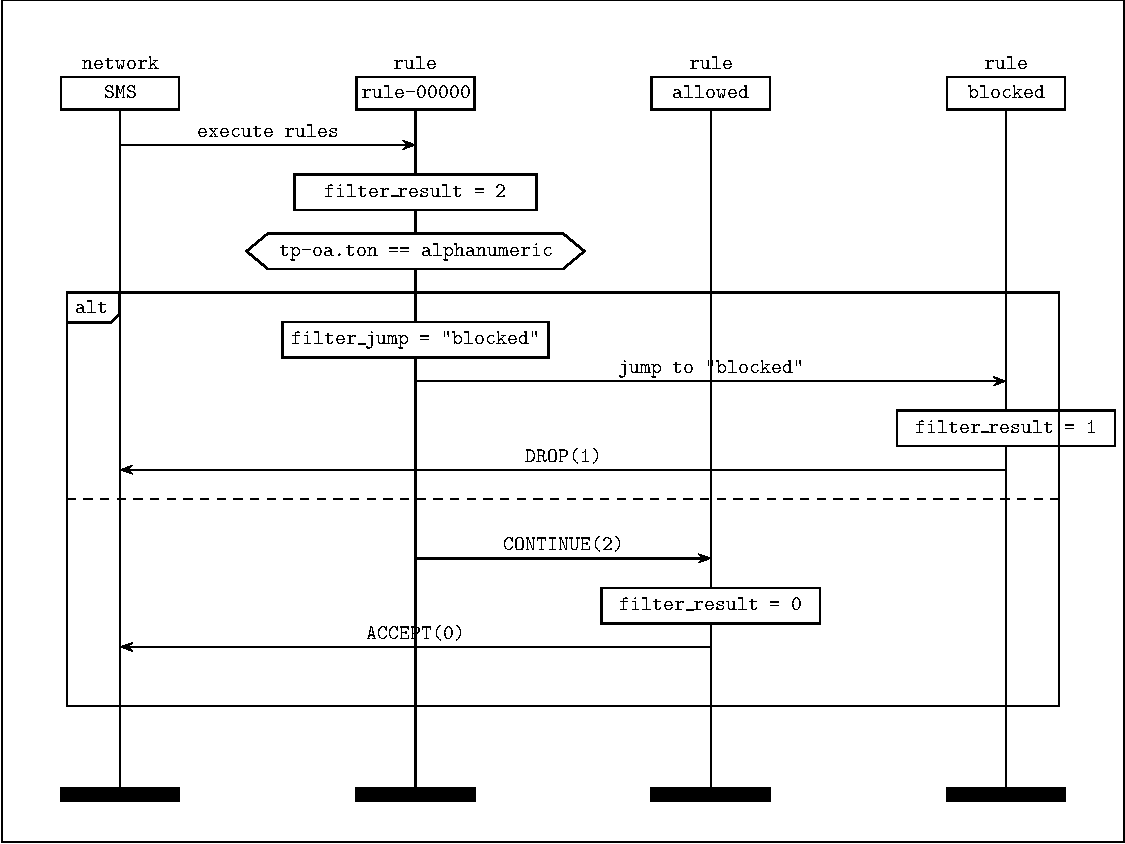
\includegraphics[width=\linewidth]{graphics/8_2_1.pdf}
\clearpage

\subsubsection{Rule match part}
Available categories in \gls{rule} \textit{"match"} section:
\begin{lstlisting}[style=BashInputStyle, belowskip=\baselineskip]
    dummy - Dummy field for generic scripting
     r14p - R14P pMINK framework data
     m3ua - MTP Level 3 (MTP3) User Adaptation Layer
     sccp - Signalling Connection Control Part      
     tcap - Transaction Capabilities Application Part
      map - Mobile Application Part                  
  smstpdu - Short message TPDU 3GPP TS 23.040
     smpp - Short Message Peer-to-Peer 
\end{lstlisting}
\noindent{}Configuration items explained:\\
\begin{tabularx}{\textwidth}{ | l | X |}
	\hline
	Item	 				& Description \\
	\hline
	\textbf{dummy}				& Context free field without default value, used only for advanced inline or external scripting \\
	\textbf{r14p}				& \acrfull{r14p} \\
	\textbf{m3ua}				& \acrfull{m3ua} \\
	\textbf{sccp}				& \acrfull{sccp} \\
	\textbf{tcap}				& \acrfull{tcap} \\
	\textbf{map}				& \acrfull{map} \\
	\textbf{smstpdu}			& \acrfull{smstpdu} \\
	\textbf{smpp}				& \acrfull{smpp} \\
	\hline
\end{tabularx}\\


\paragraph{\acrfull{r14p} matching}\label{SECTION_R14P_MATCHING}
\mbox{}\\
\acrshort{r14p} is a Release14 protocol, used for internal communication between various \acrfull{pmink} \glspl{daemon}. It is transferred via \acrfull{sctp}
as an \gls{x690} encoded \gls{asn1} data.\\

\noindent{}Configuration items listed:
\begin{lstlisting}[style=BashInputStyle, belowskip=\baselineskip]
 trunk_label - Trunk label
  service_id - Service id
    src_type - Source daemon type
      src_id - Source daemon id  
      cmd_id - Command id      
   conn_type - Source connection type
  loop_count - Loop count 
\end{lstlisting}
\noindent{}Configuration items explained:\\
\begin{tabularx}{\textwidth}{ | l | X |}
	\hline
	Item	 				& Description \\
	\hline
	\textbf{trunk\textunderscore{}label}	& Alphanumeric value assigned by \acrfull{stp}, used for mobile network traffic identification  \\ 
	\textbf{service\textunderscore{}id}	& Type of \acrshort{r14p}  ServiceMessage, a list of supported constants can be found in
                                                  section \ref{SECTION_8_2_4_4}; manual numerical equivalents are also available: 
 						  \begin{itemize}
							\setlength{\itemsep}{0pt}
							\setlength{\parskip}{0pt}
							\setlength{\parsep}{0pt}
							\item 42 - sid-openli
							\item 43 - sid-sms-data-retention
							\item 44 - sid-stp-routing
							\item 45 - sid-sgn-forward
							\item 46 - sid-smshub-forward
							\item 47 - sid-fgn-filtering
							\item 48 - sid-security
							\item 49 - sid-pdn-filtering
						  \end{itemize} \\
	\textbf{src\textunderscore{}type}	& Source \gls{daemon} type; an alphanumeric field containing an \acrshort{r14p} type of sender \\ 
	\textbf{src\textunderscore{}id}		& Source \gls{daemon} id; an alphanumeric field containing an \acrshort{r14p} id of sender \\ 
	\hline
\end{tabularx}\\
\clearpage
\noindent\begin{tabularx}{\textwidth}{ | l | X |}
	\hline
	Item	 				& Description \\
	\hline
	\textbf{cmd\textunderscore{}id}		& Special \acrfull{pmink} command id; a list of supported constants can be found in section \ref{SECTION_8_2_4_4};
						  manual numerical equivalents are also available: 
						  \begin{itemize}
							\setlength{\itemsep}{0pt}
							\setlength{\parskip}{0pt}
							\setlength{\parsep}{0pt}
							\item 1 - shci-sri-sm-req
							\item 2 - shci-sri-sm-ack
							\item 3 - shci-corr-ntf
							\item 4 - shci-sms-ack
							\item 5 - shci-sms-dlvr-rcpt
							\item 6 - shci-smpp-generate-udh
							\item 7 - shci-tcap-continue
						  \end{itemize} \\
	\textbf{conn\textunderscore{}type}	& External\footnote{Described in section \ref{SECTION_8_1}} connection type the current packet originated from; 
						  a list of supported constants can be found in section \ref{SECTION_8_2_4_4}; manual numerical equivalents are also available:
 						  \begin{itemize}
							\setlength{\itemsep}{0pt}
							\setlength{\parskip}{0pt}
							\setlength{\parsep}{0pt}
							\item 0 - UNKNOWN
							\item 1 - \acrfull{sctp}
							\item 2 - \acrfull{m3ua}
							\item 3 - \acrfull{pmink}
							\item 4 - \acrfull{tcp}
							\item 5 - \acrfull{smpp} 
						  \end{itemize} \\
	\textbf{loop\textunderscore{}count}	& Loop protection feature of \acrfull{sgn}; a numeric field indicating how many times the current packet has repeated itself \\ 
	\hline
\end{tabularx}\\


\paragraph{MTP Level 3 (MTP3) User Adaptation Layer (M3UA) matching}
\mbox{}\\
M3UA stands for MTP Level 3 (MTP3) User Adaptation Layer as defined by the IETF SIGTRAN working group in RFC 4666 (which replaces and supersedes RFC 3332). 
M3UA enables the SS7 protocol's User Parts (e.g. ISUP, SCCP and TUP) to run over IP instead of telephony equipment like ISDN and PSTN. 
It is recommended to use the services of SCTP to transmit M3UA.\\

\noindent{}Configuration items listed:
\begin{lstlisting}[style=BashInputStyle, belowskip=\baselineskip]
 opc - Originating Point Code
 dpc - Destination Point Code
  si - Service indicator     
  ni - Network indicator
  mp - Message priority 
 sls - Signalling link selection code
  as - Application Server label      
 asp - Application Server Process label
\end{lstlisting}
\noindent{}Configuration items explained:\\
\begin{tabularx}{\textwidth}{ | l | X |}
	\hline
	Item	 				& Description \\
	\hline
	\textbf{opc, dpc}			& The Originating and Destination Point Code fields contain the OPC
						  and DPC from the routing label of the original SS7 message in Network
						  Byte Order, justified to the least significant bit.  Unused bits are
						  coded `0' \\
	\textbf{si}				& The Service Indicator field contains the SI field from the original
						  SS7 message justified to the least significant bit.  Unused bits are
						  coded `0' \\
	\textbf{ni}				& The Network Indicator contains the NI field from the original SS7
   						  message justified to the least significant bit.  Unused bits are
   						  coded `0' \\ 
	\textbf{mp}				& The Message Priority field contains the MP bits (if any) from the
   						  original SS7 message, both for ANSI-style and TTC-style [29] message
   						  priority bits. The MP bits are aligned to the least significant bit.
   						  Unused bits are coded `0'\\ 
	\textbf{sls}				& The Signalling Link Selection field contains the SLS bits from the
   						  routing label of the original SS7 message justified to the least
   						  significant bit and in Network Byte Order.  Unused bits are coded
   						  `0'\\ 
	\textbf{as}				& Alphanumeric field containing an \acrfull{as} label the current packet originated from. 
						  The label was set in \acrfull{sgn} runtime configuration \\ 
	\textbf{asp}				& Alphanumeric field containing an \acrfull{asp} label the current packet originated from.
						  The label was set in \acrfull{sgn} runtime configuration \\
	\hline
\end{tabularx}

\paragraph{Signalling Connection Control Part (SCCP) matching}
\mbox{}\\
The Signalling Connection Control Part (SCCP) is a network layer protocol that provides extended routing, flow control, segmentation, connection-orientation, 
and error correction facilities in Signaling System 7 telecommunications networks. SCCP relies on the services of MTP for basic routing and error detection.

The base SCCP specification is defined by the ITU-T, in recommendations Q.711 to Q.714, with additional information to implementors provided by Q.715 and Q.716. 
There are, however, regional variations defined by local standards bodies. In the United States, ANSI publishes its modifications to Q.713 as ANSI T1.112. 
The TTC publishes as JT-Q.711 to JT-Q.714, and Europe ETSI publishes ETSI EN 300-009-1: both of which document their modifications to the ITU-T specifications.

Although MTP provides routing capabilities based upon the Point Code, SCCP allows routing using a Point Code and Subsystem number or a Global Title.
A Point Code is used to address a particular node on the network, whereas a Subsystem number addresses a specific application available on that node. SCCP employs 
a process called Global Title Translation to determine Point Codes from Global Titles so as to instruct MTP on where to route messages.

In the SIGTRAN suite of protocols, there are two primary methods of transporting SCCP applications across Internet Protocol networks: SCCP can be transported 
indirectly using the MTP level 3 User Adaptation protocol (M3UA), a protocol which provides support for users of MTP-3 including SCCP. Alternatively, SCCP applications 
can operate directly over the SCCP User Adaptation protocol (SUA) which is a form of modified SCCP designed specifically for use in IP networking.
\acrfull{sgn} uses the first method of SCCP transport; \acrfull{m3ua}.\\

\noindent{}Configuration items listed:
\begin{lstlisting}[style=BashInputStyle, belowskip=\baselineskip]
 cgpa - Calling Party
 cdpa - Called Party
\end{lstlisting}
\noindent{}Configuration sub-items listed (\textit{"cgpa/cdpa"} section):
\begin{lstlisting}[style=BashInputStyle, belowskip=\baselineskip]
 routing-indicator - Routing indicator
               gti - Global Title Indicator
               ssn - SubSystem Number
        point-code - Point code
                gt - Global Title
\end{lstlisting}
\noindent{}Configuration sub-items listed (\textit{"cgpa/cdpa gt"} section):
\begin{lstlisting}[style=BashInputStyle, belowskip=\baselineskip]
      tt - Translation type
      np - Numbering plan  
     nai - Nature Of Address
 address - GT Address
\end{lstlisting}
\noindent{}Configuration items explained:\\
\begin{tabularx}{\textwidth}{ | l | X |}
	\hline
	Item	 				& Description \\
	\hline
	\textbf{cgpa, cdpa}			& Grouping nodes, contain fields for \textit{"Calling Party Address"} and \textit{"Called Party Address"} \\ 
	\textbf{routing-indicator}		& Routing type, identifies which address element shall be used for routing: 
						  \begin{itemize} 
							\setlength{\itemsep}{0pt}
							\setlength{\parskip}{0pt}
							\setlength{\parsep}{0pt} 
							\item 0 - route on GT
							\item  1 - route on SSN
						  \end{itemize} \\
	\textbf{gti}				& Global Title Indicator field contains the type of Global Title included. A list of supported constants can be found in 
						  section \ref{SECTION_8_2_4_4}; manual numerical equivalents are also available:
						  \begin{itemize}
							\setlength{\itemsep}{0pt}
							\setlength{\parskip}{0pt}
							\setlength{\parsep}{0pt} 
							\item 0 - no global title included
							\item 4 - global title includes nature of address indicator only
							\item 8 - global title includes translation type only
							\item 12 - global title includes translation type, numbering plan and encoding scheme
							\item 16 - global title includes translation type, numbering plan, encoding scheme and nature of address indicator
						  \end{itemize} \\
	\hline
\end{tabularx}
\clearpage
\noindent\begin{tabularx}{\textwidth}{ | l | X |}
	\hline
	Item	 				& Description \\
	\hline
	\textbf{ssn}				& The Subsystem Number (SSN) is a numerical fields identifying an SCCP user function. A list of supported constants can be found in
                                                  section \ref{SECTION_8_2_4_4}; manual numerical equivalents are also available:
						  \begin{itemize}
							\setlength{\itemsep}{0pt}
							\setlength{\parskip}{0pt}
							\setlength{\parsep}{0pt} 
							\item 0 - SSN not known/not used
							\item 1 - SCCP management
							\item 2 - reserved for ITU-T allocation
							\item 3 - ISDN user part
							\item 4 - OMAP (Operation, Maintenance and Administration Part)
							\item 5 - MAP (Mobile Application Part)
							\item 6 - HLR (Home Location Register)
							\item 7 - VLR (Visitor Location Register)
							\item 8 - MSC (Mobile Switching Centre)
							\item 9 - EIC (Equipment Identifier Centre)
							\item 10 - AUC (Authentication Centre) 
							\item 11 - ISDN supplementary services
							\item 12 - reserved for international use
							\item 13 - broadband ISDN edge-to-edge applications
							\item 14 - TC test responder
						  \end{itemize} \\ 
	\textbf{point-code}			& Signalling point code (numerical) \\ 
	\textbf{gt}				& Grouping node, contains fields for \textit{"Global Title"} \\ 
	\textbf{tt}				& Translation type, a numerical value \\
	\textbf{np}				& Numbering Plan, a list of supported constants can be found in
                                                  section \ref{SECTION_8_2_4_4}; manual numerical equivalents are also available:
						  \begin{itemize}
							\setlength{\itemsep}{0pt}
							\setlength{\parskip}{0pt}
							\setlength{\parsep}{0pt} 
							\item 0 - unknown
							\item 16 - ISDN/telephony numbering plan (Recommendations E.163 and E.164)
							\item 32 - generic numbering plan
							\item 48 - data numbering plan (Recommendation X.121)
							\item 64 - telex numbering plan (Recommendation F.69
							\item 80 - maritime mobile numbering plan (Recommendations E.210, E.211)
							\item 96 - land mobile numbering plan (Recommendation E.212)
							\item 112 - ISDN/mobile numbering plan (Recommendation E.214)
							\item 224 - private network or network-specific numbering plan
						  \end{itemize} \\ 
	\textbf{nai}				& Nature Of Address, a list of supported constants can be found in
						  section \ref{SECTION_8_2_4_4}; manual numerical equivalents are also available: 
 						  \begin{itemize}
							\setlength{\itemsep}{0pt}
							\setlength{\parskip}{0pt}
							\setlength{\parsep}{0pt}
							\item 0 - unknown
							\item 1 - subscriber number
							\item 2 - reserved for national use
							\item 3 - national significant number
							\item 4 - international number
						  \end{itemize} \\ 
	\textbf{address}			& Address signals (usually digits) \\ 
	\hline
\end{tabularx}
\clearpage

\paragraph{Transaction Capabilities Application Part (TCAP) matching}
\mbox{}\\
Transaction Capabilities Application Part, from ITU-T recommendations Q.771-Q.775 or ANSI T1.114 is a protocol for Signalling System 7 networks. 
Its primary purpose is to facilitate multiple concurrent dialogs between the same sub-systems on the same machines, using Transaction IDs to differentiate 
these, similar to the way TCP ports facilitate multiplexing connections between the same IP addresses on the Internet. TCAP is used to transport INAP 
in Intelligent Networks and MAP in mobile phone networks.\\

\noindent{}Configuration items listed:
\begin{lstlisting}[style=BashInputStyle, belowskip=\baselineskip]
    tcmt - TC message type
     sid - Source transaction id
     did - Destination transaction id
      cc - Component count           
      ct - Component type 
     iid - Component invoke id
  opcode - Component operation code
 dlg_ctx - Dialogue application context
\end{lstlisting}
\noindent{}Configuration items explained:\\
\begin{tabularx}{\textwidth}{ | l | X |}
	\hline
	Item	 				& Description \\
	\hline
	\textbf{tcmt}				& TCMessage type, a list of supported constants can be found in
                                                  section \ref{SECTION_8_2_4_4}; manual numerical equivalents are also available:
 						  \begin{itemize}
							\setlength{\itemsep}{0pt}
							\setlength{\parskip}{0pt}
							\setlength{\parsep}{0pt}
							\item 1 - Unidirectional
							\item 2 - Begin
							\item 4 - End
							\item 5 - Continue
							\item 7 - Abort
						  \end{itemize} \\ 
	\textbf{sid}				& Originating Transaction ID, a numerical value present in \textit{"Begin"} and \textit{"Continue"} message types \\ 
	\textbf{did}				& Destination Transaction ID, a numerical value present in \textit{"Continue"}, \textit{"End"} and \textit{"Abort"}
						  message types \\ 
	\textbf{cc}				& ComponentPortion component count \\ 
	\textbf{ct}				& Component type,  a list of supported constants can be found in
                                                  section \ref{SECTION_8_2_4_4}; manual numerical equivalents are also available: 
 						  \begin{itemize}
							\setlength{\itemsep}{0pt}
							\setlength{\parskip}{0pt}
							\setlength{\parsep}{0pt}
							\item 1 - Invoke
							\item 2 - ReturnResultLast
							\item 3 - ReturnError
							\item 4 - Reject
							\item 7 - ReturnResultNotLast
						  \end{itemize} \\ 
	\textbf{iid}				& Invoke ID, a numerical \acrshort{tcap} reference for a specific \acrshort{tcap} operation \\ 
	\textbf{opcode}				& \acrshort{tcap} operation code, a numerical value \\ 
	\textbf{dlg\textunderscore{}ctx}	& \acrshort{tcap} Dialogue Application Context OID\\ 
	\hline
\end{tabularx}\\

\paragraph{Mobile Application Part (MAP) matching}
\mbox{}\\
The Mobile Application Part (MAP) is an SS7 protocol that provides an application layer for the various nodes in GSM and UMTS mobile core networks and GPRS core 
networks to communicate with each other in order to provide services to mobile phone users. The Mobile Application Part is the application-layer protocol used 
to access the Home Location Register, Visitor Location Register, Mobile Switching Center, Equipment Identity Register, Authentication Centre, Short message 
service center and Serving GPRS Support Node (SGSN).

The Mobile Application Part specifications were originally defined by the GSM Association, but are now controlled by ETSI/3GPP. MAP is defined by two different 
standards, depending upon the mobile network type:
\begin{itemize}
  \setlength{\itemsep}{0pt}
  \setlength{\parskip}{0pt}
  \setlength{\parsep}{0pt}
  \item MAP for GSM (prior to Release 4) is specified by 3GPP TS 09.02 (MAP v1, MAP v2)
  \item MAP for UMTS ("3G") and GSM (Release 99 and later) is specified by 3GPP TS 29.002 (MAP v3)
\end{itemize}

In cellular networks based on ANSI standards (currently CDMA2000, in the past AMPS, IS-136 and cdmaOne) plays the role of the MAP a similar protocol usually called 
IS-41 or ANSI-41 (ANSI MAP). Since 2000 it is maintained by 3GPP2 as N.S0005 and since 2004 it is named 3GPP2 X.S0004. \acrfull{pmink} supports GSM MAP v1, v2 and v3.
\clearpage

\noindent{}Configuration items listed:
\begin{lstlisting}[style=BashInputStyle, belowskip=\baselineskip]
 context - Mobile application component context
\end{lstlisting}
\noindent{}Configuration sub-items listed (\textit{"context"} section):
\begin{lstlisting}[style=BashInputStyle, belowskip=\baselineskip]
 sri-for-sm - Send routing info for short message
         sm - Short message
\end{lstlisting}
\noindent{}Configuration sub-items listed (\textit{"context sri-for-sm/sm"} section):
\begin{lstlisting}[style=BashInputStyle, belowskip=\baselineskip]
 msisdn - Mobile Station International Subscriber Directory Number
    sca - Service centre address                                  
   imsi - International mobile Subscriber Identity
    nnn - Network node number                     
     an - Additional number
\end{lstlisting}
\noindent{}Configuration sub-items listed (\textit{"context sri-for-sm/sm msisdn/sca/nnn/an/scda/scoa"} section):
\begin{lstlisting}[style=BashInputStyle, belowskip=\baselineskip]
     nai - Nature of address indicator
      np - Numbering plan            
 address - Address
\end{lstlisting}
\noindent{}Configuration items explained:\\
\begin{tabularx}{\textwidth}{ | l | X |}
	\hline
	Item	 				& Description \\
	\hline
	\textbf{context}			& Grouping node, contains fields for \textit{"sri-for-sm"} and \textit{"sm"} contexts; \textit{"sri-for-sm"} context is identified by 
						  \textbf{sendRoutingInfoForSM(45)} \acrshort{tcap} opcode value and \textit{"sm"} context by both \textbf{mt-forwardSM(44)} and 
						  \textbf{mo-forwardSM(46)} \acrshort{tcap} opcode values  \\ 
	\textbf{sri-for-sm, sm}			& Grouping nodes, contain fields for \textit{"sri-for-sm"} and \textit{"sm"} contexts \\
	\textbf{msisdn, sca, nnn, an,}		& Grouping nodes, contain fields for \textit{"Mobile Station International Subscriber Directory Number"}, \textit{"Service centre address"}, \textit{"Network node number"} and \textit{"Additional number"} \\
	\textbf{scda, scoa}			& Grouping nodes, contain fields for \textit{"Service centre address DA"} and \textit{"Service centre address OA"} \\
	\textbf{imsi}				& International mobile Subscriber Identity \\
	\textbf{nai}				& \acrfull{nai}, a list of supported constants can be found in
                                                  section \ref{SECTION_8_2_4_4}; manual numerical equivalents are also available: 
	  					  \begin{itemize}
						  	\setlength{\itemsep}{0pt}
							\setlength{\parskip}{0pt}
							\setlength{\parsep}{0pt}
							\item 0 - unknown
							\item 16 - international number
							\item 32 - national significant number
							\item 48 - network specific number
							\item 64 - subscriber number
							\item 96 - abbreviated number
						    \end{itemize} \\ 
	\textbf{np}				& \acrfull{np} Indicator, a list of supported constants can be found in
                                                  section \ref{SECTION_8_2_4_4}; manual numerical equivalents are also available: 
	  					  \begin{itemize}
						  	\setlength{\itemsep}{0pt}
							\setlength{\parskip}{0pt}
							\setlength{\parsep}{0pt}
							\item 0 - unknown
							\item 1 - ISDN/Telephony Numbering Plan (Rec ITU-T E.164)
							\item 3 - data numbering plan (ITU-T Rec X.121)
							\item 4 - telex numbering plan (ITU-T Rec F.69)
							\item 6 - land mobile numbering plan (ITU-T Rec E.212)
							\item 8 - national numbering plan
							\item 9 - private numbering plan 
						    \end{itemize} \\ 
	\textbf{address}			& Digits of an address, an alphanumeric field \\ 

	\hline
\end{tabularx}\\
\clearpage


\paragraph{Short message TPDU 3GPP TS 23.040 (SMSTPDU) matching}
\mbox{}\\
GSM 03.40 or 3GPP TS 23.040 is a mobile telephony standard describing the format of the Transfer Protocol Data Units (TPDU) of the Short Message Transfer Protocol 
(SM-TP) used in the GSM networks to carry Short Messages. This format is used throughout the whole transfer of the message in the GSM mobile network. In contrast, 
application servers use different protocols, like Short Message Peer-to-Peer or Universal Computer Protocol, to exchange messages between them and the Short message service centre.\\

GSM 03.40 is the original name of the standard. Since 1999 it is being developed by the 3GPP under the name 3GPP TS 23.040. However, the original name is often used to refer even to 
the 3GPP document.\\

The GSM 03.40 TPDUs are used to carry messages between the Mobile Station (MS) and Mobile Switching Centre (MSC) using the Short Message Relay Protocol (SM-RP), while between MSC and
a Short Message Service Centre (SMSC), the TPDUs are carried as a parameter of a Mobile Application Part (MAP) package. \acrfull{pmink} support \acrshort{smstpdu} carried 
as a \acrshort{map} parameter.\\

\noindent{}Configuration items listed:
\begin{lstlisting}[style=BashInputStyle, belowskip=\baselineskip]
        tp-rp - Reply path indicator
      tp-udhi - TP-UD header indicator
       tp-srr - MS status report request
       tp-vpf - TP-VP field format      
        tp-rd - Reject duplicates
       tp-mti - Message type indicator
        tp-mr - Message reference
       tp-sri - SME status report indicator
       tp-mms - More message to send indicator
        tp-da - Destination address
        tp-oa - Originating address
       tp-pid - Protocol identifier
       tp-dcs - Data coding scheme 
        tp-vp - Validity period
       tp-udl - Length of user data TP-UD
      tp-scts - Service centre time stamp
    ie-msg-id - Concatenated short message reference number
 ie-msg-parts - Concatenated short message total parts
  ie-msg-part - Concatenated short message part number
\end{lstlisting}
\noindent{}Configuration sub-items listed (\textit{"tp-da/tp-oa"} section):
\begin{lstlisting}[style=BashInputStyle, belowskip=\baselineskip]
     ton - Type of number
      np - Numbering plan
 address - Address
\end{lstlisting}
\noindent{}Configuration items explained:\\
\begin{tabularx}{\textwidth}{ | l | X |}
	\hline
	Item	 				& Description \\
	\hline
	\textbf{tp-rp}				& The TP-Reply-Path is a 1-bit field, located within bit no 7 of the first octet of both SMS-DELIVER and SMS-SUBMIT, 
						  and to be given the following values: 
	  					  \begin{itemize}
						  	\setlength{\itemsep}{0pt}
							\setlength{\parskip}{0pt}
							\setlength{\parsep}{0pt}
							\item 0 - TP-Reply-Path parameter is not set in this SMS-SUBMIT/DELIVER
							\item 1 - TP-Reply-Path parameter is set in this SMS-SUBMIT/DELIVER
						    \end{itemize} \\ 
	\textbf{tp-udhi}			& TP-UDHI has the following value:
 	  					  \begin{itemize}
						  	\setlength{\itemsep}{0pt}
							\setlength{\parskip}{0pt}
							\setlength{\parsep}{0pt}
							\item 0 - The TP-UD field contains only the short message
							\item 1 - The beginning of the TP-UD field contains a Header in addition to the short message
						    \end{itemize} \\ 
	\hline
\end{tabularx}
\clearpage
\noindent\begin{tabularx}{\textwidth}{ | l | X |}
	\hline
	Item	 				& Description \\
	\hline
	\textbf{tp-srr}				& The TP-Status-Report-Request is a 1-bit field, located within bit no. 5 of the first octet of SMS-SUBMIT and 
						  SMS-COMMAND, and to be given the following values: 
 	  					  \begin{itemize}
						  	\setlength{\itemsep}{0pt}
							\setlength{\parskip}{0pt}
							\setlength{\parsep}{0pt}
							\item 0 - A status report is not requested  
							\item 1 - A status report is requested 
						    \end{itemize} \\ 
	\textbf{tp-vpf}				& The TP-Validity-Period-Format is a 2-bit field, located within bit no 3 and 4 of the first octet of SMS-SUBMIT, and to 
						  be given the following values: 
 	  					  \begin{itemize}
						  	\setlength{\itemsep}{0pt}
							\setlength{\parskip}{0pt}
							\setlength{\parsep}{0pt}
							\item 0 - TP-VP field not present
							\item 16 - TP-VP field present - relative format
							\item 8 - TP-VP field present - enhanced format
							\item 24 - TP-VP field present - absolute format
						    \end{itemize} \\ 
	\textbf{tp-rd}				& The TP-Reject-Duplicates is a 1 bit field located within bit 2 of the first octet of SMS-SUBMIT and has the following 
						  values:
 	  					  \begin{itemize}
						  	\setlength{\itemsep}{0pt}
							\setlength{\parskip}{0pt}
							\setlength{\parsep}{0pt}
							\item 0 - Instruct the SC to accept an SMS-SUBMIT for an SM still held in the 
								  SC which has the same TP-MR and the same TP-DA as a previously  submitted SM from 
								  the same OA. 
							\item 1 - Instruct the SC to reject an SMS-SUBMIT for an SM still held in the 
								  SC which has the same TP-MR and the same TP-DA as the  previously submitted SM 
								  from the same OA. In this case the response returned by the SC is as specified in \acrfull{smstpdu}, section 9.2.3.6
						    \end{itemize} \\ 
	\textbf{tp-mti}				& The TP-Message-Type-Indicator is a 2-bit field, located within bits no 0 and 1 of the first octet of all PDUs which can 
						  be given the following values:
 	  					  \begin{itemize}
						  	\setlength{\itemsep}{0pt}
							\setlength{\parskip}{0pt}
							\setlength{\parsep}{0pt}
							\item 0 - SMS-DELIVER
							\item 1 - SMS-DELIVER-REPORT
							\item 2 - SMS-SUBMIT
							\item 3 - SMS-SUBMIT-REPORT
							\item 4 - SMS-STATUS-REPORT
							\item 5 - SMS-COMMAND
						    \end{itemize} \\ 
	\textbf{tp-mr}				& The TP-Message-Reference field gives an integer representation of a reference number of the SMS-SUBMIT or 
						  SMS-COMMAND submitted to the SC by the MS. The MS increments TP-Message-Reference by 1 for each 
						  SMS-SUBMIT or SMS-COMMAND being submitted \\
	\textbf{tp-sri}				& The TP-Status-Report-Indication is a 1-bit field, located within bit no. 5 of the first octet of SMS-DELIVER, and to be 
						  given the following values:
 	  					  \begin{itemize}
						  	\setlength{\itemsep}{0pt}
							\setlength{\parskip}{0pt}
							\setlength{\parsep}{0pt}
							\item 0 - A status report shall not be returned to the SME  
							\item 1 - A status report shall be returned to the SME
						    \end{itemize} \\ 
	\textbf{tp-mms}				& The TP-More-Messages-to-Send is a 1-bit field, located within bit no 2 of the first octet of SMS-DELIVER and 
						  SMS-STATUS-REPORT, and to be given the following values:
 	  					  \begin{itemize}
						  	\setlength{\itemsep}{0pt}
							\setlength{\parskip}{0pt}
							\setlength{\parsep}{0pt}
							\item 0 - More messages are waiting for the MS in this SC
							\item 1 - No more messages are waiting for the MS in this SC
						    \end{itemize} \\ 
	\textbf{tp-da, tp-oa}			& Grouping nodes, contain fields for \textit{"TP-Destination-Address"} and \textit{"TP-Originating-Address"} \\ 
	\textbf{tp-pid}				& The TP-Protocol-Identifier is the information element by which the SM-TL either refers to the higher layer protocol being 
						  used, or indicates interworking with a certain type of telematic device \\ 
	\textbf{tp-dcs}				& TP-Data-Coding-Scheme represents a character set being used for \acrshort{sms} text. A list of supported constants can be found in
                                                  section \ref{SECTION_8_2_4_4}; manual numerical equivalents are also available:
 	  					  \begin{itemize}
						  	\setlength{\itemsep}{0pt}
							\setlength{\parskip}{0pt}
							\setlength{\parsep}{0pt}
							\item 0 - GSM 7 bit default alphabet
							\item 4 - 8 bit data
							\item 8 - UCS2 (16bit)
						    \end{itemize} \\ 
	\hline
\end{tabularx}
\clearpage
\noindent\begin{tabularx}{\textwidth}{ | l | X |}
	\hline
	Item	 				& Description \\
	\hline
	\textbf{tp-vp}				& The TP-Validity-Period comprises 1 octet in integer representation, giving the length of the validity period, counted 
						  from when the SMS-SUBMIT is received by the SC. \acrfull{pmink} automatically converts all 3 types of validity period formats
						  to UNIX timestamp. This field contains a maximum timestamp value for which the \acrshort{sms} is still considered valid\\ 
	\textbf{tp-udl}				& If the TP-User-Data is coded using the GSM 7 bit default alphabet, the TP-User-Data-Length field gives an integer 
						  representation of the number of septets within the TP-User-Data field to follow. If the 7bit default-alphabet extension 
						  mechanism is used within the TP-User-Data (see 3GPP TS 23.038 [9]), the actual number of characters in the message 
						  shall be less than the number of septets. If a TP-User-Data-Header field is present, then the TP-User-Data-Length value 
						  is the sum of the number of septets in the TP-User-Data-Header field (including any padding) and the number of septets 
						  in the TP-User-Data field which follows. If the TP-User-Data is coded using 8-bit data, the 
						  TP-User-Data-Length field gives an integer representation of the number of octets within the TP-User-Data field to 
						  follow. If a TP-User-Data-Header field is present, then the TP-User-Data-Length value is the sum of the number of 
						  octets in the TP-User-Data-Header field and the number of octets in the TP-User-Data field which follows.
						  If the TP-User-Data is coded using UCS2 [24] data, the TP-User-Data-Length field gives an integer representation of 
						  the number of octets within the TP-User-Data field to follow. If a TP-User-Data-Header field is present, then the 
						  TP-User-Data-Length value is the sum of the number of octets in the TP-User-Data-Header field and the number of 
						  octets in the TP-User-Data field which follows. \\ 
	\textbf{tp-scts}			& TP-Service-Centre-Time-Stamp converted to UNIX timestamp\\ 
	\textbf{ie-msg-id}			& Concatenated short message reference number\\ 
	\textbf{ie-msg-parts}			& Maximum number of short messages in the concatenated short message \\ 
	\textbf{ie-msg-part}			& Sequence number of the current short message within the concatenated short message \\ 
	\textbf{ton}				& \acrfull{ton}, a list of supported constants can be found in
                                                  section \ref{SECTION_8_2_4_4}; manual numerical equivalents are also available: 
	  					  \begin{itemize}
						  	\setlength{\itemsep}{0pt}
							\setlength{\parskip}{0pt}
							\setlength{\parsep}{0pt}
							\item 0 - Unknown
							\item 16 - International number
							\item 32 - National number
							\item 48 - Network specific number
							\item 64 - Subscriber number
							\item 80 - Alphanumeric, (coded according to 3GPP TS 23.038 [9] GSM 7-bit default alphabet)
							\item 96 - Abbreviated number
							\item 112 - Reserved for extension
						    \end{itemize} \\ 
	\textbf{np}				& \acrfull{np}, a list of supported constants can be found in
                                                  section \ref{SECTION_8_2_4_4}; manual numerical equivalents are also available: 
	  					  \begin{itemize}
						  	\setlength{\itemsep}{0pt}
							\setlength{\parskip}{0pt}
							\setlength{\parsep}{0pt}
							\item 0 - Unknown
							\item 1 - ISDN/telephone numbering plan (E.164 [17]/E.163[18])
							\item 3 - Data numbering plan (X.121)
							\item 4 - Telex numbering plan
							\item 6 - Land mobile numbering plan
							\item 8 - National numbering plan
							\item 9 - Private numbering plan
							\item 10 - ERMES numbering plan (ETSI DE/PS 3 01-3)
							\item 15 - Reserved for extension
						    \end{itemize} \\ 
	\textbf{address}			& Address digits \\

	\hline
\end{tabularx}
\clearpage

\paragraph{Short Message Peer-to-Peer (SMPP) matching}
\mbox{}\\
The Short Message Peer-to-Peer (SMPP) in the telecommunications industry is an open, industry standard protocol designed to provide a flexible data communication interface 
for the transfer of short message data between External Short Messaging Entities (ESME), Routing Entities (RE) and Message Centres.\\

SMPP is often used to allow third parties (e.g. value-added service providers like news organizations) to submit messages, often in bulk, but it may be used for SMS peering as well. 
SMPP is able to carry short messages including EMS, Voice Mail notifications, Cell Broadcasts, WAP messages including WAP Push messages (used to deliver MMS notifications), USSD 
messages and others. Because of its versatility and support for non-GSM SMS protocols, like UMTS, IS-95 (CDMA), CDMA2000, ANSI-136 (TDMA) and iDEN, the SMPP is the most commonly 
used protocol for short message exchange outside SS7 networks.\\

\acrfull{pmink} uses \acrfull{sgn} as the main entry point and external\footnote{Described in section \ref{SECTION_8_1}} signalling converter. \acrfull{smpp} connections follow the
same organizational principles as \acrfull{m3ua} connections by using both \acrfull{as} logical entities and \acrfull{asp} instances.\\

\noindent{}Configuration items listed:
\begin{lstlisting}[style=BashInputStyle, belowskip=\baselineskip]
                      as - Application Server label
                     asp - Application Server Process label
              command_id - SMPP PDU message type
         source_addr_ton - Address type of number
           dest_addr_ton - Address type of number
         source_addr_npi - Address numbering plan indicator
           dest_addr_npi - Address numbering plan indicator
             source_addr - SME originating address
        destination_addr - SME destination address
            esm_class_mm - ESM class message mode
            esm_class_mt - ESM class message type
           esm_class_gsm - ESM class GSM network specific features
             protocol_id - Protocol identifier according to GSM 03.40
           priority_flag - Short message priority level
           delivery_time - Scheduled time at which the message delivery should be first attempted
         validity_period - Validity period
       rd_smsc_dlvr_rcpt - SMSC Delivery Receipt
         rd_sme_orig_ack - SME originated Acknowledgement
           rd_intrmd_ntf - Intermediate Notification
 replace_if_present_flag - Request SMSC to replace a previously submitted message
             data_coding - Short message data coding
       sm_default_msg_id - SMSC index of a pre-defined (canned) message
               sm_length - Length of short_message parameter in octets
         sar_msg_ref_num - Reference number for a particular concatenated short message
      sar_total_segments - Total number of short messages within the concatenated short message
      sar_segment_seqnum - Sequence number of a particular short message within the concatenated short message
\end{lstlisting}
\noindent{}Configuration items explained:\\
\begin{tabularx}{\textwidth}{ | l | X |}
	\hline
	Item	 								& Description \\
	\hline
	\textbf{as}								& Alphanumeric field containing an \acrfull{as} label the current packet originated from. 
						  				  The label was set in \acrfull{sgn} runtime configuration \\ 
	\textbf{asp}								& Alphanumeric field containing an \acrfull{asp} label the current packet originated from. \\
	\hline
\end{tabularx}
\clearpage
\noindent\begin{tabularx}{\textwidth}{ | l | X |}
	\hline
	Item	 								& Description \\
	\hline
	\textbf{command\textunderscore{}id}					& The command\textunderscore{}id field identifies the type of message the SMPP PDU represents, for example, 
										  submit\textunderscore{}sm, query\textunderscore{}sm etc. A command identifier is allocated to 
										  each SMPP request primitive. A list of supported constants can be found in section \ref{SECTION_8_2_4_4}; manual 
										  numerical equivalents are also available: \\
										& \\
										& {
										  \begin{tabularx}{12cm}{  r l }
										    2147483648		&	GENERIC\textunderscore{}NACK \\
										    1			&	BIND Operation - BIND\textunderscore{}RECEIVER \\
										    2147483649      	&       BIND Operation - BIND\textunderscore{}RECEIVER\textunderscore{}RESP \\
										    2  			&	BIND Operation - BIND\textunderscore{}TRANSMITTER \\
										    2147483650  	&	BIND Operation - BIND\textunderscore{}TRANSMITTER\textunderscore{}RESP \\
										    3            	&	QUERY\textunderscore{}SM Operation - QUERY\textunderscore{}SM \\
										    2147483651   	&	QUERY\textunderscore{}SM Operation - QUERY\textunderscore{}SM\textunderscore{}RESP \\
										    4 			&	SUBMIT\textunderscore{}SM Operation - SUBMIT\textunderscore{}SM \\
										    2147483652     	&	SUBMIT\textunderscore{}SM Operation - SUBMIT\textunderscore{}SM\textunderscore{}RESP \\
										    5           	&	DELIVER\textunderscore{}SM Operation - DELIVER\textunderscore{}SM \\
										    2147483653   	&	DELIVER\textunderscore{}SM Operation - DELIVER\textunderscore{}SM\textunderscore{}RESP \\
										    6        		&	UNBIND Operation - UNBIND \\
										    2147483654 		&	UNBIND Operation - UNBIND\textunderscore{}RESP \\
										    7               	&	REPLACE\textunderscore{}SM Operation - REPLACE\textunderscore{}SM \\
										    2147483655      	&	REPLACE\textunderscore{}SM Operation - REPLACE\textunderscore{}SM\textunderscore{}RESP \\
										    8               	&	CANCEL\textunderscore{}SM Operation - CANCEL\textunderscore{}SM \\
										    2147483656      	&	CANCEL\textunderscore{}SM Operation - CANCEL\textunderscore{}SM\textunderscore{}RESP \\
										    9               	&	BIND Operation - BIND\textunderscore{}TRANSCEIVER \\
										    2147483657      	&	BIND Operation - BIND\textunderscore{}TRANSCEIVER\textunderscore{}RESP \\
										    11              	&	OUTBIND Operation - OUTBIND \\
										    21              	&	ENQUIRE\textunderscore{}LINK Operation - ENQUIRE\textunderscore{}LINK \\
										    2147483669      	&	ENQUIRE\textunderscore{}LINK Operation - ENQUIRE\textunderscore{}LINK\textunderscore{}RESP \\
										    33              	&	SUBMIT\textunderscore{}MULTI Operation - SUBMIT\textunderscore{}MULTI \\
										    2147483681      	&	SUBMIT\textunderscore{}MULTI Operation - SUBMIT\textunderscore{}MULTI\textunderscore{}RESP \\
										    258             	&	ALERT\textunderscore{}NOTIFICATION Operation - ALERT\textunderscore{}NOTIFICATION \\
										    259             	&	DATA\textunderscore{}SM Operation - DATA\textunderscore{}SM \\
										    2147483907      	&	DATA\textunderscore{}SM Operation - DATA\textunderscore{}SM\textunderscore{}RESP \\
										  \end{tabularx}
										  } \\
										& \\
	\textbf{source\textunderscore{}addr\textunderscore{}ton}	 	& \acrfull{ton}, a list of supported constants can be found in  section \ref{SECTION_8_2_4_4}; \\
	\textbf{dest\textunderscore{}addr\textunderscore{}ton}			& manual numerical equivalents are also available: 
	  					  				  \begin{itemize}
			  						  	    \setlength{\itemsep}{0pt}
										    \setlength{\parskip}{0pt}
										    \setlength{\parsep}{0pt}
										    \item 0 - Unknown
										    \item 1 - International
										    \item 2 - National
										    \item 3 - Network Specific
										    \item 4 - Subscriber Number
										    \item 5 - Alphanumeric
										    \item 6 - Abbreviated
						    				  \end{itemize} \\ 
	\textbf{source\textunderscore{}addr\textunderscore{}npi}	 	& \acrfull{np} Indicator, a list of supported constants can be found in \\
	\textbf{dest\textunderscore{}addr\textunderscore{}npi}			& in section \ref{SECTION_8_2_4_4}; manual numerical equivalents are also \\
										& available:
	  					  				  \begin{itemize}
			  						  	    \setlength{\itemsep}{0pt}
										    \setlength{\parskip}{0pt}
										    \setlength{\parsep}{0pt}
										    \item 0 - Unknown
										    \item 1 - ISDN (E163/E164)
										    \item 3 - Data (X.121)
										    \item 4 - Telex (F.69)
										    \item 6 - Land Mobile (E.212)
										    \item 8 - National
										    \item 9 - Private
										    \item 10 - ERMES
										    \item 14 - Internet (IP)
										    \item 18 - WAP Client Id (to be defined by WAP Forum) 
						    				  \end{itemize} \\ 


	\hline
\end{tabularx}\\
\clearpage
\noindent\begin{tabularx}{\textwidth}{ | l | X |}
	\hline
	Item	 								& Description \\
	\hline
	\textbf{source\textunderscore{}addr}	 				& Specifies the address of SME which originated this message. An ESME which is implemented 
										  as a single SME address, may set this field to NULL to allow the SMSC to default the source 
										  address of the submitted message. \\ 
	\textbf{destination\textunderscore{}addr}				& Specifies the destination SME address. For mobile terminated messages, this is the directory 
										  number of the recipient MS. \\ 
	\textbf{esm\textunderscore{}class\textunderscore{}mm}			& The esm\textunderscore{}class\textunderscore{}mm parameter is used to indicate special message mode attribute 
										  associated with the short message. A list of supported constants can be found in  section \ref{SECTION_8_2_4_4};
										  manual numerical equivalents are also available: 
	  					  				  \begin{itemize}
			  						  	    \setlength{\itemsep}{0pt}
										    \setlength{\parskip}{0pt}
										    \setlength{\parsep}{0pt}
										    \item 0 - Default SMSC Mode (e.g. Store and Forward)
										    \item 1 - Datagram mode
										    \item 2 - Forward (i.e. Transaction) mode
										    \item 3 - Store and Forward mode (use to select Store and Forward mode if Default SMSC Mode is non Store and Forward
						    				  \end{itemize} \\ 
	\textbf{esm\textunderscore{}class\textunderscore{}mt}			& The esm\textunderscore{}class\textunderscore{}mt parameter is used to indicate special message type attribute associated 
										  with the short message. A list of supported constants can be found in  section \ref{SECTION_8_2_4_4};
										  manual numerical equivalents are also available: 
	  					  				  \begin{itemize}
			  						  	    \setlength{\itemsep}{0pt}
										    \setlength{\parskip}{0pt}
										    \setlength{\parsep}{0pt}
										    \item 0 - Default message Type (i.e. normal message)
										    \item 4 - Short Message contains SMSC Delivery Receipt
										    \item 8 - Short Message contains ESME Delivery Acknowledgement
										    \item 16 - Short Message contains ESME Manual/User Acknowledgement
										    \item 24 - Short Message contains Conversation Abort (Korean CDMA)
										    \item 32 - Short Message contains Intermediate Delivery Notification
						    				  \end{itemize} \\ 
	\textbf{esm\textunderscore{}class\textunderscore{}gsm}			& The esm\textunderscore{}class\textunderscore{}gsm parameter is used to indicate special GSM attribute associated 
										  with the short message. A list of supported constants can be found in  section \ref{SECTION_8_2_4_4};
										  manual numerical equivalents are also available: 
	  					  				  \begin{itemize}
			  						  	    \setlength{\itemsep}{0pt}
										    \setlength{\parskip}{0pt}
										    \setlength{\parsep}{0pt}
										    \item 0 - No specific features selected
										    \item 64 - UDHI Indicator (only relevant for MT short messages)
										    \item 128 - Set Reply Path (only relevant for GSM network)
										    \item 192 - Set UDHI and Reply Path (only relevant for GSM network)
						    				  \end{itemize} \\ 
	\textbf{protocol\textunderscore{}id}					& A numerical value set according to GSM 03.40 \\
	\textbf{priority\textunderscore{}flag}					& The priority\textunderscore{}flag parameter allows the originating SME to assign a priority level to the short
										  message. Four priority levels are supported;
										  manual numerical equivalents are also available: 
	  					  				  \begin{itemize}
			  						  	    \setlength{\itemsep}{0pt}
										    \setlength{\parskip}{0pt}
										    \setlength{\parsep}{0pt}
										    \item 0 - Level 0 (lowest) priority
										    \item 1 - Level 1 priority
										    \item 2 - Level 2 priority
										    \item 3 - Level 3 (highest) priority
						    				  \end{itemize} \\
	\textbf{delivery\textunderscore{}time}					& This parameter specifies the scheduled time at which the message delivery should be first
										  attempted. It defines either the absolute date and time or relative time from the current SMSC time at which
										  delivery of this message will be attempted by the SMSC. This is a numerical field; \acrfull{pmink} converts both 
										  Absolute and Relative time formats of scheduled\textunderscore{}delivery\textunderscore{}time to UNIX timestamp. \\
	\textbf{validity\textunderscore{}period}				& The validity\textunderscore{}period parameter indicates the SMSC expiration time, after which the message
										  should be discarded if not delivered to the destination. This is a numerical field; \acrfull{pmink} converts both 
                                                                                  Absolute and Relative time formats of validity\textunderscore{}period to UNIX timestamp \\

	\hline
\end{tabularx}
\clearpage
\noindent\begin{tabularx}{\textwidth}{ | l | X |}
	\hline
	Item	 									& Description \\
	\hline
	\textbf{rd\textunderscore{}smsc\textunderscore{}dlvr\textunderscore{}rcpt}	& The rd\textunderscore{}smsc\textunderscore{}dlvr\textunderscore{}rcpt parameter is used to request an SMSC delivery receipt.
											  A list of supported constants can be found in  section \ref{SECTION_8_2_4_4};
											  manual numerical equivalents are also available: 
	  					  				  	  \begin{itemize}
			  						  	    	    \setlength{\itemsep}{0pt}
										    	    \setlength{\parskip}{0pt}
										    	    \setlength{\parsep}{0pt}
										    	    \item 0 - No SMSC Delivery Receipt requested (default)
											    \item 1 - SMSC Delivery Receipt requested where final delivery outcome is delivery success or failure
											    \item 2 - SMSC Delivery Receipt requested where the final delivery outcome is delivery failure
						    				  	  \end{itemize} \\ 
	\textbf{rd\textunderscore{}sme\textunderscore{}orig\textunderscore{}ack}	& The rd\textunderscore{}sme\textunderscore{}orig\textunderscore{}ack parameter is used to request an SME originated acknowledgements.
											  A list of supported constants can be found in  section \ref{SECTION_8_2_4_4};
											  manual numerical equivalents are also available: 
	  					  				  	  \begin{itemize}
			  						  	    	    \setlength{\itemsep}{0pt}
										    	    \setlength{\parskip}{0pt}
										    	    \setlength{\parsep}{0pt}
										    	    \item 0 - No recipient SME acknowledgment requested (default)
											    \item 4 - SME Delivery Acknowledgement requested
											    \item 8 - SME Manual/User Acknowledgment requested
											    \item 12 - Both Delivery and Manual/User Acknowledgment requested
						    				  	  \end{itemize} \\ 
	\textbf{rd\textunderscore{}intrmd\textunderscore{}ntf}				& The rd\textunderscore{}inrmd\textunderscore{}ntf parameter is used to request an SMSC intermediate notification.
											  A list of supported constants can be found in  section \ref{SECTION_8_2_4_4};
											  manual numerical equivalents are also available: 
	  					  				  	  \begin{itemize}
			  						  	    	    \setlength{\itemsep}{0pt}
										    	    \setlength{\parskip}{0pt}
										    	    \setlength{\parsep}{0pt}
										    	    \item 0 - No Intermediate notification requested (default)
											    \item 16 - Intermediate notification requested
						    				  	  \end{itemize} \\ 
	\textbf{replace\textunderscore{}if\textunderscore{}present\textunderscore{}flag}& The replace\textunderscore{}if\textunderscore{}present\textunderscore{}flag parameter is used to request the SMSC 
											  to replace a previously submitted message, that is still pending delivery. The SMSC will replace an existing message 
											  provided that the source address, destination address and service\textunderscore{}type match the same fields in the new message.
											  The following values are supported;
	  					  				  	  \begin{itemize}
				  						  	    \setlength{\itemsep}{0pt}
										    	    \setlength{\parskip}{0pt}
										    	    \setlength{\parsep}{0pt}
										    	    \item 0 - Don't replace (default)
											    \item 1 - Replace
						    				  	  \end{itemize} \\
	\textbf{data\textunderscore{}coding}						& \acrshort{sms} text data coding scheme, a list of supported constants can be found in  section \ref{SECTION_8_2_4_4};
											  manual numerical equivalents are also available: 
	  					  				  	  \begin{itemize}
			  						  	    	    \setlength{\itemsep}{0pt}
										    	    \setlength{\parskip}{0pt}
										    	    \setlength{\parsep}{0pt}
										    	    \item 0 - SMSC Default Alphabet
											    \item 1 - IA5 (CCITT T.50)/ASCII (ANSI X3.4)
											    \item 2 - Octet unspecified (8-bit binary)
											    \item 3 - Latin 1 (ISO-8859-1)
											    \item 4 - Octet unspecified (8-bit binary)
											    \item 5 - JIS (X 0208-1990)
											    \item 6 - Cyrllic (ISO-8859-5)
											    \item 7 - Latin/Hebrew (ISO-8859-8)
											    \item 8 - UCS2 (ISO/IEC-10646)
											    \item 9 - Pictogram Encoding
											    \item 10 - ISO-2022-JP (Music Codes)
											    \item 13 - Extended Kanji JIS(X 0212-1990
											    \item 14 - KS C 5601
						    				  	  \end{itemize} \\ 
	\textbf{sm\textunderscore{}default\textunderscore{}msg\textunderscore{}id}	& The sm\textunderscore{}default\textunderscore{}msg\textunderscore{}id parameter specifies the SMSC index of 
											  a pre-defined (canned) message \\
	\textbf{sm\textunderscore{}length}						& The sm\textunderscore{}length parameter specifies the length of the short\textunderscore{}message parameter in octets. 
											  The sm\textunderscore{}length should be set to 0 in the submit\textunderscore{}sm, submit\textunderscore{}multi, and 
											  deliver\textunderscore{}sm PDUs if the message\textunderscore{}payload parameter is being used to send user data 
											  larger than 254 octets. \\


	\hline
\end{tabularx}
\clearpage
\noindent\begin{tabularx}{\textwidth}{ | l | X |}
	\hline
	Item	 									& Description \\
	\hline
	\textbf{sar\textunderscore{}msg\textunderscore{}ref\textunderscore{}num}	& The sar\textunderscore{}msg\textunderscore{}ref\textunderscore{}num parameter is used to indicate the reference 
											  number for a particular concatenated short message.\\
	\textbf{sar\textunderscore{}total\textunderscore{}segments}			& The sar\textunderscore{}total\textunderscore{}segments parameter is used to indicate the total number of short messages 
  											  within the concatenated short message. \\
	\textbf{sar\textunderscore{}segment\textunderscore{}seqnum}			& The sar\textunderscore{}segment\textunderscore{}seqnum parameter is used to indicate the sequence number of a particular 
											  short message within the concatenated short message. \\
	\hline
\end{tabularx}

\subsubsection{Basic matching}
\acrfull{fgn} \acrfull{rpe} supports two levels of parameter matching; \textit{basic} and \textit{advanced}. 
Basic matching, implemented as an extension of a standard set of \gls{boolean} operators, is further extended with 
\Gls{perl} compatible regular expressions and \acrshort{pmink} specific field modifiers. 

\paragraph{Basic matching syntax}\label{SECTION_BASIC_SYNTAX}
\mbox{}\\
\vspace{0.5cm}
\[
	\text{config\textunderscore{}item}\tikzmark{cfgitem} \; "[LC\tikzmark{lciop}I] \quad O\tikzmark{op}P \quad @\tikzmark{var} \; [RC\tikzmark{rciop}I] \quad \text{operand\textunderscore{}B}\tikzmark{operand}"
\]
\begin{tikzpicture}[overlay,remember picture, thick]
  % nodes
  \node(n1) at ( $ (pic cs:lciop) +(-3cm,-2cm) $ ) {Left component index modifier};
  \node(n2) at ( $ (pic cs:op) +(-0cm,-2cm) $ ) {Operator};
  \node(n3) at ( $ (pic cs:var) +(-3pt,-3.5cm) $ ) {Symbol for \acrshort{pmink} constant or variable};
  \node(n4) at ( $ (pic cs:rciop) +(3cm,-2.5cm) $ ) {Right component index modifier};
  \node(n5) at ( $ (pic cs:operand) +(-0.5cm,-1.2cm) $ ) {Right operand};
  \node(n6) at ( $ (pic cs:cfgitem) +(-1cm,-1cm) $ ) {Left operand};
  
  % optional
  \draw [decorate,decoration={brace,amplitude=10pt}] ( $ (pic cs:lciop) +(-0.6cm,0.4cm) $ ) -- ( $ (pic cs:rciop) +(0.3cm,0.4cm) $ ) node [above, midway, yshift=0.2cm] {optional};

  % paths
  \path[->] (n1) edge [bend right, yshift=-2pt, color=blue] 				(pic cs:lciop);
  \path[->] (n2) edge [yshift=-2pt, color=orange] 					(pic cs:op);
  \path[->] (n3) edge [yshift=-2pt, xshift=-3pt, color=pink] 				(pic cs:var);
  \path[->] (n4) edge [bend left, yshift=-2pt, xshift=-3pt, color=blue] 		(pic cs:rciop);
  \path[->] (n5) edge [yshift=-2pt, xshift=-0.5cm, color=orange] 			(pic cs:operand);
  \path[->] (n6) edge [xshift=-1cm, yshift=-2pt, color=green] 			(pic cs:cfgitem);

\end{tikzpicture}
\vspace{4cm}

\noindent{}The syntax explained in this chapter focues on the lowest configuration level; a configuration item(\textit{"config\textunderscore{}item"}) represents an 
external\footnotemark or internal\footnotemark[\value{footnote}] signalling data available
for matching. Data matching is a process of comparing a relation between two operands(\underline{left} and \underline{right}); in case of basic matching, the first 
operand(\underline{left}) is not under user control and always points to a runtime configuration item(\textit{"config\textunderscore{}item"}).\\
\footnotetext{Described in section \ref{SECTION_8_1}}
The second operand(\underline{right}), displayed as \textit{"operand\textunderscore{}B"} in this diagram, can be accessed and maintained through \acrfull{cli}, and is 
entirely under user control. Several different operand types are supported; their purpose and format will be covered in the following chapters. \\

The relationship between two operands is examined by creating a relational expression whose result evaluates to \textbf{"true"} or \textbf{"false"}, 
depending on operator \textit{"OP"}. This evaluation result is used by \acrfull{rproc}\footnote{Described in section \ref{SECTION_8_2}} to determine the next step 
in \gls{rule} execution flow. Basic syntax, used in \textit{"match"} section of runtime configuration, features two extra components; \underline{left} and \underline{right} 
component index modifiers(\textit{"\acrshort{lci}"} and \textit{"\acrshort{rci}"}).\\

\acrlong{pdu}s sometimes contain multiple instances of various parameters; \acrfull{sgn} generates numerical \gls{zbased} indexes to differentiate between those parameters.
\acrfull{lci}, used for selecting a specific instance of runtime configuration item(\textit{"config\textunderscore{}item"}), uses \gls{zbased} indexes received from \acrshort{sgn}.
Both left and right component index modifiers operate on the same set of indexes; the only difference between the two is that \acrfull{rci} is used exclusively with predefined
\acrshort{pmink} variables.\\

\noindent{}Most components of basic syntax are optional; if they are not used, default values are automatically selected.
\begin{tabularx}{\textwidth}{ | r | X |}
	\hline
	Basic syntax component 		& Default value \\
	\hline
	\acrfull{lci}			& 0(zero) \\
	Operator \textit{"OP"}		& ==(equality) \\
	\acrfull{rci}			& 0(zero) \\
	\hline
\end{tabularx}\\
\clearpage
\noindent{}Example rule (\textit{"match tcap"} section):
\begin{lstlisting}[style=BashInputStyle, belowskip=\baselineskip]
config@hostname:/configure/mno/fgn/fgn1/rules/rule-00000/definition/match/tcap > configuration 
tcmt    "@tcap.const.tcmt_end"
ct      "[0]!=@tcap.const.ct_error"
\end{lstlisting}
\noindent\fbox{%
\begin{minipage}{\linewidth-2\fboxsep-2\fboxrule}
Explanation of \textit{"match tcap tcmt"} field:
\[
	\text{tcmt}\tikzmark{cfgitem2} \; \quad @\tikzmark{var2} \; \text{tcap.const.tcmt\textunderscore{}end}\tikzmark{operand2}"
\]
\begin{tikzpicture}[overlay,remember picture, thick]
  % nodes
  \node(2n3) at ( $ (pic cs:var2) +(-3pt,-2cm) $ ) {Symbol for \acrshort{pmink} constant or variable};
  \node(2n5) at ( $ (pic cs:operand2) +(1.5cm,-1.2cm) $ ) {Right operand(\acrshort{pmink} constant)};
  \node(2n6) at ( $ (pic cs:cfgitem2) +(-2.5cm,-1cm) $ ) {Left operand};

  % paths
  \path[->] (2n3) edge [yshift=-2pt, xshift=-3pt, color=pink] 				(pic cs:var2);
  \path[->] (2n5) edge [bend left=10, yshift=-2pt, xshift=-12pt, color=orange] 		(pic cs:operand2);
  \path[->] (2n6) edge [bend right=10, xshift=-8pt, yshift=-2pt, color=green] 		(pic cs:cfgitem2);

\end{tikzpicture}
\vspace{2cm}

\mbox{}\\
\begin{tabularx}{\linewidth}{ | r | X |}
	\hline
	Basic syntax component 			& Value \\
	\hline
	Left operand				& tcmt \\ 
	\acrfull{lci}				& 0(zero) \\
	Operator \textit{"OP"}			& ==(equality) \\
	\acrshort{pmink} variable/constant	& yes \\
	\acrfull{rci}				& 0(zero) \\
	Right operand				& tcap.const.tcmt\textunderscore{}end \\
	\hline
\end{tabularx}%
\mbox{}\\

\noindent{}Description:\\
Check if \acrfull{tcap} TCMessage is of type "End"
\end{minipage}%
}
\vspace{1cm}

\noindent\fbox{%
\begin{minipage}{\linewidth-2\fboxsep-2\fboxrule}
Explanation of \textit{"match tcap ct"} field:
\[
	\text{ct}\tikzmark{cfgitem3} \; "[0\tikzmark{lciop3}] \quad \text{!=}\tikzmark{op3} \quad @\tikzmark{var3} \; \text{tcap.const.ct\textunderscore{}error}\tikzmark{operand3}"
\]
\begin{tikzpicture}[overlay,remember picture, thick]
  % nodes
  \node(3n1) at ( $ (pic cs:lciop3) +(-3cm,-2cm) $ ) {Left component index modifier};
  \node(3n2) at ( $ (pic cs:op3) +(-40pt,-2.8cm) $ ) {Operator(inequality)};
  \node(3n3) at ( $ (pic cs:var3) +(-3pt,-4cm) $ ) {Symbol for \acrshort{pmink} constant or variable};
  \node(3n5) at ( $ (pic cs:operand3) +(0cm,-1.2cm) $ ) {Right operand(\acrshort{pmink} constant)};
  \node(3n6) at ( $ (pic cs:cfgitem3) +(-2.5cm,-1cm) $ ) {Left operand};

  % paths
  \path[->] (3n1) edge [bend right, yshift=-2pt, xshift=-2pt, color=blue]		(pic cs:lciop3);
  \path[->] (3n2) edge [bend right, yshift=-2pt, xshift=-6pt,color=orange] 		(pic cs:op3);
  \path[->] (3n3) edge [yshift=-2pt, xshift=-3pt, color=pink] 				(pic cs:var3);
  \path[->] (3n5) edge [bend left=10, yshift=-2pt, xshift=-50pt, color=orange] 		(pic cs:operand3);
  \path[->] (3n6) edge [bend right=10, xshift=-8pt, yshift=-2pt, color=green] 		(pic cs:cfgitem3);

\end{tikzpicture}
\vspace{4cm}

\mbox{}\\
\begin{tabularx}{\textwidth}{ | r | X |}
	\hline
	Basic syntax component 			& Value \\
	\hline
	Left operand				& ct \\ 
	\acrfull{lci}				& 0(zero) \\
	Operator \textit{"OP"}			& !=(inequality) \\
	\acrshort{pmink} variable/constant	& yes \\
	\acrfull{rci}				& 0(zero) \\
	Right operand				& tcap.const.ct\textunderscore{}error \\
	\hline
\end{tabularx}%
\mbox{}\\

\noindent{}Description:\\
Check if \acrfull{tcap} component at index 0 is anything other than ReturnError
\end{minipage}%
}
\clearpage
\paragraph{Operand types}
\mbox{}\\
\acrfull{pmink} basic syntax supports 6 types of operands; all of them are supported in {\textit{"match"}\footnotemark} section and only some in {\textit{"translate"}\footnotemark[\value{footnote}]} section.
\footnotetext{Described in section \ref{SECTION_8_2}}

\subparagraph{NUMBER type operand}\label{SECTION_NUMBER}
is a numerical operand consisting of one or more digits.\\

\noindent{}Example rule (\textit{"match tcap"} section):
\begin{lstlisting}[style=BashInputStyle, belowskip=\baselineskip]
config@hostname:/configure/mno/fgn/fgn1/rules/rule-00000/definition/match/tcap > configuration 
tcmt    "4"
\end{lstlisting}
Description:\\
Check if \acrfull{tcap} TCMessage is of type associated with number 4

\subparagraph{STRING type operand}\label{SECTION_STRING}
is a sequence of characters enclosed in matching single quotes(')\footnote{String operands be used, although not recommended, without single quotes}.\\

\noindent{}Example rule (\textit{"match smstpdu} section):
\begin{lstlisting}[style=BashInputStyle, belowskip=\baselineskip]
config@hostname:/configure/mno/fgn/fgn1/rules/rule-00000/definition/match/smstpdu > configuration 
tp-oa {
        address "'38670007007'"                          
}
\end{lstlisting}
Description:\\
Check if \acrfull{smstpdu} \acrfull{tp-oa} address digits match "38670007007"

\subparagraph{REGEX type operand}\label{SECTION_REGEX}
is a \Gls{perl} compatible \Gls{regex} indicated by a sequence of characters starting with a colon(:) sign; more detailed information can be found on the following address: \url{http://perldoc.perl.org/perlre.html\#Regular-Expressions}\\

\noindent{}Example rule (\textit{"match m3ua"} section):
\begin{lstlisting}[style=BashInputStyle, belowskip=\baselineskip]
config@hostname:/configure/mno/fgn/fgn1/rules/rule-00000/definition/match/m3ua > configuration
opc ":(?=^..25).*"
\end{lstlisting}
Description:\\
Check if \acrfull{m3ua} Originating Point Code starts with any two characters followed by "25"\\

\noindent{}\textbf{Note:} When using REGEX type operand, \acrfull{rci} and operator \textit{"OP"} are not supported; \gls{regex} always operates on left operand (\textit{"config\_item")} and evaluates to \textbf{"true"} if match is found.

\subparagraph{VARIABLE type operand}\label{SECTION_VARIABLE} if a special \acrshort{pmink} predefined variable or constant, indicated by a sequence of characters starting with at(@) sign. 
A list of supported values can be found in section \ref{SECTION_8_2_4_4}.\\

\noindent{}Example rule (\textit{"match m3ua"} section):
\begin{lstlisting}[style=BashInputStyle, belowskip=\baselineskip]
config@hostname:/configure/mno/fgn/fgn1/rules/rule-00000/definition/match/smstpdu > configuration 
tp-oa {
        ton     "@smstpdu.const.noa_alphanumeric"
}
\end{lstlisting}
Description:\\
Check if \acrfull{smstpdu} \acrfull{tp-oa} \acrfull{ton} is alphanumeric
\clearpage

\subparagraph{LIST type operand} is a special \acrshort{pmink} operand used for referencing two types of lists; \textit{"static"}\footnote{Described in section \ref{SECTION_8_1_3_3}} and 
\textit{"dynamic"}\footnote{Described in section \ref{SECTION_DYN_LISTS}}. It is implemented as an extension of variable type operand; a list is referenced by using an at(@) sign followed by sequence of characters enclosed in curly brackets.\\

\noindent{}Example rule (\textit{"match sccp"} section):
\begin{lstlisting}[style=BashInputStyle, belowskip=\baselineskip]
config@hostname:/configure/mno/fgn/fgn1/rules/rule-00000/definition/match/sccp > configuration 
cgpa {
        gt {
                address "@{gt_black_list}"
        }                                   
}
\end{lstlisting}
Description:\\
Check if \acrfull{sccp} Calling Party Global Title address exists in a list named "gt\_black\_list"

\subparagraph{LUA type operand}\label{SECTION_LUA_OPERAND}
is an external scripting feature used for extending basic syntax and features of \acrfull{fgn}; \acrfull{pmink} uses \Gls{lua} programming language as a powerful and simple solution for \acrshort{fgn} customization.
\Gls{lua} type operand is indicated by two consecutive grave accent(\`{}) signs followed by inline scripting block or absolute path to external script. This topic will be discussed in more detail starting from section 
\ref{SECTION_8_2_5}.\\

\noindent{}Example rule (\textit{"match sccp"} section):
\begin{lstlisting}[style=BashInputStyle, belowskip=\baselineskip, upquote=true]
config@hostname:/configure/mno/fgn/fgn1/rules/rule-00000/definition/match/sccp > configuration 
cgpa {
        gt {
                address "``return F.sl_get('gt_black_list', F.vpval())"
        }                                   
}
\end{lstlisting}
Description:\\
Check if \acrfull{sccp} Calling Party Global Title address exists in a list named "gt\_black\_list"

\paragraph{Operator types}
\mbox{}\\
\acrfull{pmink} supports 6 relational and 3 content-changing operators; the latter provide a basic syntax interface to advanced list manipulation techniques.

\subparagraph{Equality '==' operator}
evaluates to \textbf{"true"} if both left and right operands are equal.\\

\noindent{}Example rule (\textit{"match map"} section):
\begin{lstlisting}[style=BashInputStyle, belowskip=\baselineskip, upquote=true]
config@hostname:/configure/mno/fgn/fgn1/rules/rule-00000/definition/match/map > configuration 
context {
        sm {
                scda {
                        nai     "==@map.const.noa_international"
                }
        }        
}
\end{lstlisting}
Description:\\
Check if \acrfull{sms} ServiceCentreAddressDA \acrfull{nai} is set to international"
\clearpage

\subparagraph{Inequality '!=' operator}
evaluates to \textbf{"true"} if both left and right operands are different.\\

\noindent{}Example rule (\textit{"match map"} section):
\begin{lstlisting}[style=BashInputStyle, belowskip=\baselineskip, upquote=true]
config@hostname:/configure/mno/fgn/fgn1/rules/rule-00000/definition/match/map > configuration 
context {
        sm {
                scda {
                        np      "!=@map.const.np_national"
                }
        }        
}
\end{lstlisting}
Description:\\
Check if \acrfull{sms} ServiceCentreAddressDA \acrfull{np} is anything other than national"

\subparagraph{Greater than '\textgreater' operator}
evaluates to \textbf{"true"} if left operand is greater than the right operand.\\

\noindent{}Example rule (\textit{"match m3ua"} section):
\begin{lstlisting}[style=BashInputStyle, belowskip=\baselineskip, upquote=true]
config@hostname:/configure/mno/fgn/fgn1/rules/rule-00000/definition/match/m3ua > configuration 
dpc ">5000"
\end{lstlisting}
Description:\\
Check if \acrfull{m3ua} Destination Point Code is greater than 5000"

\subparagraph{Greater than equal '\textgreater{}=' operator}
evaluates to \textbf{"true"} if left operand is greater than or equal to the right operand.\\

\noindent{}Example rule (\textit{"match m3ua"} section):
\begin{lstlisting}[style=BashInputStyle, belowskip=\baselineskip, upquote=true]
config@hostname:/configure/mno/fgn/fgn1/rules/rule-00000/definition/match/m3ua > configuration 
opc ">=4000"
\end{lstlisting}
Description:\\
Check if \acrfull{m3ua} Originating Point Code is greater than or equal to 4000"

\subparagraph{Less than '\textless' operator}
evaluates to \textbf{"true"} if left operand is less than the right operand.\\

\noindent{}Example rule (\textit{"match m3ua"} section):
\begin{lstlisting}[style=BashInputStyle, belowskip=\baselineskip, upquote=true]
config@hostname:/configure/mno/fgn/fgn1/rules/rule-00000/definition/match/m3ua > configuration 
dpc "<5000"
\end{lstlisting}
Description:\\
Check if \acrfull{m3ua} Destination Point Code is less than 5000"

\subparagraph{Less than equal '\textless{}=' operator}
evaluates to \textbf{"true"} if left operand is less than or equal to the right operand.\\

\noindent{}Example rule (\textit{"match m3ua"} section):
\begin{lstlisting}[style=BashInputStyle, belowskip=\baselineskip, upquote=true]
config@hostname:/configure/mno/fgn/fgn1/rules/rule-00000/definition/match/m3ua > configuration 
opc "<=4000"
\end{lstlisting}
Description:\\
Check if \acrfull{m3ua} Originating Point Code is less than or equal to 4000"
\clearpage

\subparagraph{Add to list '\textgreater\textgreater' operator}\label{ROT-LST-ADD}
is a special type of operator used exclusively for adding data to both static and dynamic lists; data contained in left operand is added to the listed 
specified by right operand. The resulting expression will always evaluate to \textbf{"true"}.\\

\noindent{}Example rule (\textit{"match sccp"} section):
\begin{lstlisting}[style=BashInputStyle, belowskip=\baselineskip, upquote=true]
config@hostname:/configure/mno/fgn/fgn1/rules/rule-00000/definition/match/sccp > configuration 
cdpa {
        gt {
                address ">>@{gt_black_list}"
        }                                   
}
\end{lstlisting}
Description:\\
Add \acrfull{sccp} Called Party Global Title address to a list named "gt\_black\_list"

\subparagraph{Remove from list '\textless\textless' operator}
is another special type of operator used exclusively for removing data from both static and dynamic lists; data contained in left operand is removed from the listed 
specified by right operand. The resulting expression will always evaluate to \textbf{"true"}.\\

\noindent{}Example rule (\textit{"match sccp"} section):
\begin{lstlisting}[style=BashInputStyle, belowskip=\baselineskip, upquote=true]
config@hostname:/configure/mno/fgn/fgn1/rules/rule-00000/definition/match/sccp > configuration 
cdpa {
        gt {
                address "<<@{gt_black_list}"
        }                                   
}
\end{lstlisting}
Description:\\
Remove \acrfull{sccp} Called Party Global Title address from a list named "gt\_black\_list"

\subparagraph{Remove list '\textendash\textendash' operator}
is the last special type of operator used exclusively for removing both static and dynamic lists; a list specified by right operand is cleared and removed. 
The resulting expression will always evaluate to \textbf{"true"}.\\

\noindent{}Example rule (\textit{"match"} section):
\begin{lstlisting}[style=BashInputStyle, belowskip=\baselineskip, upquote=true]
config@hostname:/configure/mno/fgn/fgn1/rules/rule-00000/definition/match > configuration 
dummy "--@{gt_black_list}"
\end{lstlisting}
Description:\\
Remove a list named "gt\_black\_list"\\

\noindent{}\textbf{Note:} \textbf{"dummy"} is a special runtime configuration field used in cases like this one, when left operand is not needed or ignored

\paragraph{Predefined constants and variables}\label{SECTION_8_2_4_4}
\mbox{}\\
\acrfull{pmink} features a set of predefined constants and variables to provide a more human friendly way of referencing certain protocol fields and/or
parameters. 


\clearpage
\noindent
\begin{tabularx}{\linewidth}{ | >{\ttfamily} r | >{\ttfamily} X |}
	\hline
	\acrshort{pmink} variable		& Value \\
	\hline
	\rowcolor{blue!10}
	\multicolumn{2}{| l |}{\acrfull{pmink}}	\\
	\hline
	pmink.timestamp				& Current UNIX timetstamp \\ 
	\hline
	\rowcolor{blue!10}
	\multicolumn{2}{| l |}{\acrfull{smpp}} 	\\
	\hline
	smpp.command\_id			& SMPP PDU message type \\
	smpp.source\_addr\_ton			& Source address type of number\\
	smpp.dest\_addr\_ton			& Destination address type of number\\
	smpp.source\_addr\_npi			& Source address numbering plan indicator\\
	smpp.dest\_addr\_npi			& Destination address numbering plan indicator\\
	smpp.source\_addr			& SME originating address\\
	smpp.destination\_addr			& SME destination address\\
	smpp.esm\_class\_mm			& ESM class message mode\\
	smpp.esm\_class\_mt			& ESM class message type\\
	smpp.esm\_class\_gsm			& ESM class GSM network specific features\\
	smpp.protocol\_id			& Protocol identifier according to GSM 03.40\\
	smpp.priority\_flag			& Short message priority level\\
	smpp.delivery\_time			& Scheduled time at which the delivery should be first attempted\\
	smpp.validity\_period			& Validity period\\
	smpp.rd\_smsc\_dlvr\_rcpt		& SMSC Delivery Receipt\\
	smpp.rd\_sme\_orig\_ack			& SME originated Acknowledgement\\
	smpp.rd\_intrmd\_ntf			& Intermediate Notification\\
	smpp.replace\_if\_present\_flag		& Request SMSC to replace a previously submitted message\\
	smpp.data\_coding			& Short message data coding\\
	smpp.sm\_default\_msg\_id		& SMSC index of a pre-defined (canned) message\\
	smpp.sm\_length				& Length of short\_message parameter in octets\\
	smpp.sar\_msg\_ref\_num			& Reference number for a particular concatenated short message\\
	smpp.sar\_total\_segments		& Number of messages within the concatenated message\\
	smpp.sar\_segment\_seqnum		& Message sequence number within the concatenated message\\
	\hline
	\rowcolor{blue!10}
	\multicolumn{2}{| l |}{\acrfull{tcap}} 	\\
	\hline
	tcap.tcmt				& TCAP message type\\
	tcap.sid				& Source transaction id\\
	tcap.did				& Destination transaction id\\
	tcap.cc					& Component count\\
	tcap.ct					& Component type\\
	tcap.iid				& Component invoke id\\
	tcap.opcode				& Component operation code\\
	tcap.dlg\_ctx				& Dialogue application context\\
	\hline
	\rowcolor{blue!10}
	\multicolumn{2}{| l |}{\acrfull{map}} 	\\
	\hline
	map.imsi				& International mobile Subscriber Identity\\
	map.msisdn.nai				& MSISDN Nature of address indicator\\
	map.msisdn.np				& MSISDN Numbering plan\\
	map.msisdn.address			& MSISDN address digits\\
	map.sca.nai				& Service centre address Nature of address indicator\\
	map.sca.np				& Service centre address Numbering plan \\
	map.sca.address				& Service centre address digits\\
	map.scoa.nai				& Service centre address OA Nature of address indicator\\
	map.scoa.np				& Service centre address OA Numbering plan\\
	map.scoa.address			& Service centre address OA digits\\
	map.scda.nai				& Service centre address DA Nature of address indicator\\
	map.scda.np				& Service centre address DA Numbering plan\\
	map.scda.address			& Service centre address DA digits\\
	map.nnn.nai				& Network node number Nature of address indicator\\
	map.nnn.np				& Network node number Numbering plan\\
	map.nnn.address				& Network node number digits\\
	map.an.nai				& Additional number Nature of address indicator\\
	map.an.np				& Additional number Numbering plan\\
	map.an.address				& Additional number digits\\
	\hline
\end{tabularx}%
\clearpage

\noindent
\begin{tabularx}{\linewidth}{ | >{\ttfamily} r | >{\ttfamily} X |}
	\hline
	\rowcolor{blue!10}
	\multicolumn{2}{| l |}{\acrfull{smstpdu}} 	\\
	\hline
	smstpdu.tp-rp					& Reply path indicator\\
	smstpdu.tp-udhi					& TP-UD header indicator\\
	smstpdu.tp-srr					& MS status report request\\
	smstpdu.tp-vpf					& TP-VP field format\\
	smstpdu.tp-rd					& Reject duplicates\\
	smstpdu.tp-mti					& Message type indicator\\
	smstpdu.tp-mr					& Message reference\\
	smstpdu.tp-sri					& SME status report indicator\\
	smstpdu.tp-mms					& More message to send indicator\\
	smstpdu.tp-da.ton				& Destination address Type Of Number\\
	smstpdu.tp-da.np				& Destination address Numbering Plan\\
	smstpdu.tp-da.address				& Destination address digits\\
	smstpdu.tp-oa.ton				& Originating address Type Of Number\\
	smstpdu.tp-oa.np				& Originating address Numbering Plan\\
	smstpdu.tp-oa.address				& Originating address digits\\
	smstpdu.tp-pid					& Protocol identifier\\
	smstpdu.tp-dcs					& Data coding scheme\\
	smstpdu.tp-vp					& Validity period\\
	smstpdu.tp-udl					& Length of user data TP-UD\\
	smstpdu.tp-scts					& Service centre time stamp\\
	smstpdu.ie.msg\_id				& Concatenated short message reference number\\
	smstpdu.ie.msg\_parts				& Concatenated short message total parts\\
	smstpdu.ie.msg\_part				& Concatenated short message part number\\
	\hline
	\rowcolor{blue!10}
	\multicolumn{2}{| l |}{\acrfull{m3ua}} 		\\
	\hline
	m3ua.opc					& Originating Point Code\\
	m3ua.dpc					& Destination Point Code\\
	m3ua.si						& Service indicator\\
	m3ua.ni						& Network indicator\\
	m3ua.mp						& Message priority\\
	m3ua.sls					& Signalling link selection code\\
	m3ua.as						& Application Server label\\
	m3ua.asp					& Application Server Process label\\
	\hline
	\rowcolor{blue!10}
	\multicolumn{2}{| l |}{\acrfull{sccp}} 		\\
	\hline
	sccp.cgpa.routing-indicator			& Calling Party Address Routing indicator\\
	sccp.cgpa.gti					& Calling Party Address Global Title Indicator\\
	sccp.cgpa.ssn					& Calling Party Address SubSystem Number\\
	sccp.cgpa.point-code				& Calling Party Address Point code\\
	sccp.cgpa.gt.tt					& Calling Party Address Global Title Translation type\\
	sccp.cgpa.gt.np					& Calling Party Address Global Title Numbering plan\\
	sccp.cgpa.gt.nai				& Calling Party Address Global Title Nature Of Address\\
	sccp.cgpa.gt.address				& Calling Party Address Global Title digits\\
	sccp.cdpa.routing-indicator			& Called Party Address Routing indicator\\
	sccp.cdpa.gti					& Called Party Address Global Title Indicator\\
	sccp.cdpa.ssn					& Called Party Address SubSystem Number\\
	sccp.cdpa.point-code				& Called Party Address Point code\\
	sccp.cdpa.gt.tt					& Called Party Address Global Title Translation type\\
	sccp.cdpa.gt.np					& Called Party Address Global Title Numbering plan\\
	sccp.cdpa.gt.nai				& Called Party Address Global Title Nature Of Address\\
	sccp.cdpa.gt.address				& Called Party Address Global Title digits\\
	\hline
\end{tabularx}%
\clearpage

\noindent
\begin{tabularx}{\linewidth}{ | >{\ttfamily} r | >{\ttfamily} X |}
	\hline	
	\acrshort{pmink} constant			& Value \\
	\hline
	\rowcolor{blue!10}
	\multicolumn{2}{| l |}{\acrfull{r14p}} 	\\
	\hline
	r14p.const.srvcid\_openli			& Service id 42 - sid-openli\\
	r14p.const.srvcid\_sms\_dr			& Service id 43 - sid-sms-data-retention\\
	r14p.const.srvcid\_stp\_routing			& Service id 44 - sid-stp-routing\\
	r14p.const.srvcid\_sgn\_fwd			& Service id 45 - sid-sgn-forward\\
	r14p.const.srvcid\_smshub\_fwd			& Service id 46 - sid-smshub-forward\\
	r14p.const.srvcid\_fgn\_filtering		& Service id 47 - sid-fgn-filtering\\
	r14p.const.srvcid\_security			& Service id 48 - sid-security\\
	r14p.const.srvcid\_pdn\_filtering		& Service id 49 - sid-pdn-filtering\\	
	r14p.const.cmdid\_srism\_req			& Command id 1 - shci-sri-sm-req\\
	r14p.const.cmdid\_srism\_ack			& Command id 2 - shci-sri-sm-ack\\
	r14p.const.cmdid\_corr\_ntf			& Command id 3 - shci-corr-ntf\\
	r14p.const.cmdid\_sms\_ack			& Command id 4 - shci-sms-ack\\
	r14p.const.cmdid\_sms\_dlvr\_rcpt		& Command id 5 - shci-sms-dlvr-rcpt\\
	r14p.const.cmdid\_smpp\_generate\_udh		& Command id 6 - shci-smpp-generate-udh\\
	r14p.const.cmdid\_tcap\_continue		& Command id 7 - shci-tcap-continue\\
	r14p.const.connt\_sctp				& Source connection type 1 - \acrshort{sctp}\\
	r14p.const.connt\_m3ua				& Source connection type 2 - \acrshort{m3ua}\\
	r14p.const.connt\_tcp				& Source connection type 4 - \acrshort{tcp}\\
	r14p.const.connt\_smpp				& Source connection type 5 - \acrshort{smpp}\\
	\hline
	\rowcolor{blue!10}
	\multicolumn{2}{| l |}{\acrfull{smpp}} 	\\
	\hline
	smpp.const.command\_generic\_nack		& PDU type 0x80000000 - GENERIC\_NACK\\
	smpp.const.command\_bind\_receiver		& PDU type 0x00000001 - BIND\_RECEIVER\\
	smpp.const.command\_bind\_receiver\_resp	& PDU type 0x80000001 - BIND\_RECEIVER\_RESP\\
	smpp.const.command\_bind\_transmitter		& PDU type 0x00000002 - BIND\_TRANSMITTER\\
	smpp.const.command\_bind\_transmitter\_resp	& PDU type 0x80000002 - BIND\_TRANSMITTER\_RESP\\
	smpp.const.command\_query\_sm			& PDU type 0x00000003 - QUERY\_SM\\
	smpp.const.command\_query\_sm\_resp		& PDU type 0x80000003 - QUERY\_SM\_RESP\\
	smpp.const.command\_submit\_sm			& PDU type 0x00000004 - SUBMIT\_SM\\
	smpp.const.command\_submit\_sm\_resp		& PDU type 0x80000004 - SUBMIT\_SM\_RESP\\
	smpp.const.command\_deliver\_sm			& PDU type 0x00000005 - DELIVER\_SM\\
	smpp.const.command\_deliver\_sm\_resp		& PDU type 0x80000005 - DELIVER\_SM\_RESP\\
	smpp.const.command\_unbind			& PDU type 0x00000006 - UNBIND\\
	smpp.const.command\_unbind\_resp		& PDU type 0x80000006 - UNBIND\_RESP\\
	smpp.const.command\_replace\_sm			& PDU type 0x00000007 - REPLACE\_SM\\
	smpp.const.command\_replace\_sm\_resp		& PDU type 0x80000007 - REPLACE\_SM\_RESP\\
	smpp.const.command\_cancel\_sm			& PDU type 0x00000008 - CANCEL\_SM\\
	smpp.const.command\_cancel\_sm\_resp		& PDU type 0x80000008 - CANCEL\_SM\_RESP\\
	smpp.const.command\_bind\_transceiver		& PDU type 0x00000009 - BIND\_TRANSCEIVER\\
	smpp.const.command\_bind\_transceiver\_resp	& PDU type 0x80000009 - BIND\_TRANSCEIVER\_RESP\\
	smpp.const.command\_outbind			& PDU type 0x0000000B - OUTBIND\\
	smpp.const.command\_enquire\_link		& PDU type 0x00000015 - ENQUIRE\_LINK\\
	smpp.const.command\_enquire\_link\_resp		& PDU type 0x80000015 - ENQUIRE\_LINK\_RESP\\
	smpp.const.command\_submit\_multi		& PDU type 0x00000021 - SUBMIT\_MULTI\\
	smpp.const.command\_submit\_multi\_resp		& PDU type 0x80000021 - SUBMIT\_MULTI\_RESP\\
	smpp.const.command\_alert			& PDU type 0x00000102 - ALERT\_NOTIFICATION\\
	smpp.const.command\_data\_sm			& PDU type 0x00000103 - DATA\_SM\\
	smpp.const.command\_data\_sm\_resp		& PDU type 0x80000103 - DATA\_SM\_RESP\\
	smpp.const.ton\_unknown				& Type Of Number - 0 - Unknown\\
	smpp.const.ton\_international			& Type Of Number - 1 - International\\
	smpp.const.ton\_national			& Type Of Number - 2 - National\\
	smpp.const.ton\_network\_specific		& Type Of Number - 3 - Network Specific\\
	smpp.const.ton\_subscriber			& Type Of Number - 4 - Subscriber Number\\
	smpp.const.ton\_alphanumeric			& Type Of Number - 5 - Alphanumeric\\
	smpp.const.ton\_abbreviated			& Type Of Number - 6 - Abbreviated\\
	smpp.const.npi\_unknown				& Numbering Plan - 0 - Unknown\\
	smpp.const.npi\_isdn\_telephone			& Numbering Plan - 1 - ISDN (E163/E164)\\
	smpp.const.npi\_data\_x121			& Numbering Plan - 3 - Data (X.121)\\
	smpp.const.npi\_telex				& Numbering Plan - 4 - Telex (F.69)\\
	\hline
\end{tabularx}%
\clearpage

\noindent
\begin{tabularx}{\linewidth}{ | >{\ttfamily} r | >{\ttfamily} X |}
	\hline
	smpp.const.npi\_land\_mobile			& Numbering Plan - 6 - Land Mobile (E.212)\\
	smpp.const.npi\_national			& Numbering Plan - 8 - National\\
	smpp.const.npi\_private				& Numbering Plan - 9 - Private\\
	smpp.const.npi\_ermes				& Numbering Plan - 10 - ERMES\\
	smpp.const.npi\_internet\_ip			& Numbering Plan - 14 - Internet (IP)\\
	smpp.const.npi\_wap\_client\_id			& Numbering Plan - 18 - WAP Client Id\\
	smpp.const.dc\_default				& Data coding - 0 - SMSC Default Alphabet\\
	smpp.const.dc\_ia5\_ascii			& Data coding - 1 - IA5 (CCITT T.50)/ASCII\\
	smpp.const.dc\_8bit\_binary\_1			& Data coding - 2 - 8-bit binary\\
	smpp.const.dc\_iso\_8859\_1			& Data coding - 3 - Latin 1 (ISO-8859-1)\\
	smpp.const.dc\_8bit\_binary\_2			& Data coding - 4 - 8-bit binary\\
	smpp.const.dc\_jis				& Data coding - 5 - JIS (X 0208-1990)\\
	smpp.const.dc\_8859\_5				& Data coding - 6 - Cyrllic (ISO-8859-5)\\
	smpp.const.dc\_8859\_8				& Data coding - 7 - Latin/Hebrew (ISO-8859-8)\\
	smpp.const.dc\_ucs2				& Data coding - 8 - UCS2 (ISO/IEC-10646)\\
	smpp.const.dc\_pictogram			& Data coding - 9 - Pictogram Encoding\\
	smpp.const.dc\_iso\_2011\_jp			& Data coding - 10 - ISO-2022-JP (Music Codes)\\
	smpp.const.dc\_extended\_kanji			& Data coding - 13 - Extended Kanji JIS\\
	smpp.const.dc\_ks\_c\_5601			& Data coding - 14 - KS C 5601\\
	smpp.const.gsm\_no\_features			& GSM - No specific features selected\\
	smpp.const.gsm\_udhi				& GSM - UDHI Indicator\\
	smpp.const.gsm\_reply\_path			& GSM - Set Reply Path\\
	smpp.const.gsm\_udhi\_reply\_path		& GSM - Set UDHI and Reply Path\\
	smpp.const.int\_no				& No Intermediate notification requested\\
	smpp.const.int\_yes				& Intermediate notification requested\\
	smpp.const.mm\_default\_smsc			& ESM class MM - Default SMSC\\
	smpp.const.mm\_datagram				& ESM class MM - Datagram mode\\
	smpp.const.mm\_forward				& ESM class MM - Forward (Transaction) mode\\
	smpp.const.mm\_store\_forward			& ESM class MM - Store and Forward mode\\
	smpp.const.mst\_enroute				& Message state - Enroute\\
	smpp.const.mst\_delivered			& Message state - Delivered\\
	smpp.const.mst\_expired				& Message state - Expired\\
	smpp.const.mst\_deleted				& Message state - Deleted\\
	smpp.const.mst\_undeliverable			& Message state - Undeliverable\\
	smpp.const.mst\_accepted			& Message state - Accepted\\
	smpp.const.mst\_unknown				& Message state - Unknown\\
	smpp.const.mst\_rejected			& Message state - Rejected\\
	smpp.const.mt\_default				& ESM class MT - Default message Type\\
	smpp.const.mt\_smsc\_delivery\_rcpt		& ESM class MT - SMSC Delivery Receipt\\
	smpp.const.mt\_delivery\_ack			& ESM class MT - ESME Delivery Ack\\
	smpp.const.mt\_manual\_user\_ack		& ESM class MT - ESME Manual/User Ack\\
	smpp.const.mt\_cnvrs\_abort			& ESM class MT - Conversation Abort\\
	smpp.const.mt\_intrm\_dlvr\_ntf			& ESM class MT - Intermediate Delivery Notification\\
	smpp.const.soa\_no\_sme\_ack			& SME Ack - No SME Ack\\
	smpp.const.soa\_sme\_ack			& SME Ack - SME Ack Requested\\
	smpp.const.soa\_sme\_manual\_user\_ack		& SME Ack - SME Manual/User Ack\\
	smpp.const.soa\_sme\_both			& SME Ack - Delivery and Manual/User Ack \\
	smpp.const.sdr\_no\_smsc\_delivery		& No SMSC Delivery Receipt\\
	smpp.const.sdr\_success\_failure		& SMSC Delivery Receipt success or failure\\
	smpp.const.sdr\_failure				& SMSC Delivery Receipt failure\\
	smpp.const.si\_not\_screened			& Screening Indicator - not screened\\
	smpp.const.si\_verified\_passed			& Screening Indicator - verified and passed\\
	smpp.const.si\_verified\_failed			& Screening Indicator - verified and failed\\
	smpp.const.si\_network\_provided		& Screening Indicator - network provided\\
	smpp.const.pi\_allowed				& Presentation Indicator - allowed\\
	smpp.const.pi\_restricted			& Presentation Indicator - restricted\\
	smpp.const.pi\_not\_available			& Presentation Indicator - n/a\\
	smpp.const.dfr\_destination\_unavailable	& Delivery Failure Reason - destination n/a\\
	smpp.const.dfr\_destination\_address\_invalid	& Delivery Failure Reason - address invalid\\
	smpp.const.dfr\_perm\_net\_err			& Delivery Failure Reason - permanent error\\
	\hline
\end{tabularx}%
\clearpage

\noindent
\begin{tabularx}{\linewidth}{ | >{\ttfamily} r | >{\ttfamily} X |}
	\hline
	smpp.const.dfr\_temp\_net\_err			& Delivery Failure Reason - temporary error\\
	smpp.const.das\_unknown				& Dest Addr Subunit Type - Unknown\\
	smpp.const.das\_ms\_display			& Dest Addr Subunit Type - MS Display\\
	smpp.const.das\_mobile\_equipment		& Dest Addr Subunit Type - Mobile Equipment\\
	smpp.const.das\_smart\_card\_1			& Dest Addr Subunit Type - Smart Card 1\\
	smpp.const.das\_external\_unit\_1		& Dest Addr Subunit Type - External Unit 1\\
	smpp.const.db\_unknown				& Dest Bearer Type - Unknown\\
	smpp.const.db\_sms				& Dest Bearer Type - SMS\\
	smpp.const.db\_csd				& Dest Bearer Type - Circuit Switched Data\\	
	smpp.const.db\_packet\_data			& Dest Bearer Type - Packet Data\\
	smpp.const.db\_ussd				& Dest Bearer Type - USSD\\
	smpp.const.db\_cdpd				& Dest Bearer Type - CDPD\\
	smpp.const.db\_data\_tac			& Dest Bearer Type - DataTAC\\
	smpp.const.db\_flex\_reflex			& Dest Bearer Type - FLEX/ReFLEX\\
	smpp.const.db\_cell\_broadcast			& Dest Bearer Type - Cell Broadcast\\
	smpp.const.dn\_unknown				& Dest Network Type - Unknown\\
	smpp.const.dn\_gsm				& Dest Network Type - GSM\\
	smpp.const.dn\_ansi\_136			& Dest Network Type - ANSI-136/TDM\\
	smpp.const.dn\_is\_95				& Dest Network Type - IS-95/CDMA\\
	smpp.const.dn\_pdc				& Dest Network Type - PDC\\
	smpp.const.dn\_phs				& Dest Network Type - PHS\\
	smpp.const.dn\_iden				& Dest Network Type - iDEN\\
	smpp.const.dn\_amps				& Dest Network Type - AMPS\\
	smpp.const.dn\_paging\_network			& Dest Network Type - Paging Network\\
	smpp.const.ds\_nsap\_even			& Dest Subaddress Type - NSAP (Even) [ITUT X.213]\\
	smpp.const.ds\_nsap\_odd			& Dest Subaddress Type - NSAP (Odd) [ITUT X.213]\\
	smpp.const.ds\_user\_specified			& Dest Subaddress Type - User specified\\
	smpp.const.dt\_temporary			& Display Time - Temporary\\
	smpp.const.dt\_default				& Display Time - Default\\
	smpp.const.dt\_invoke				& Display Time - Invoke\\
	smpp.const.irc\_digit				& Its Reply Type - Digit\\
	smpp.const.irc\_number				& Its Reply Type - Number\\
	smpp.const.irc\_telephone\_no			& Its Reply Type - Telephone No.\\
	smpp.const.irc\_password			& Its Reply Type - Password\\
	smpp.const.irc\_char\_line			& Its Reply Type - Character Line\\
	smpp.const.irc\_menu				& Its Reply Type - Menu\\
	smpp.const.irc\_date				& Its Reply Type - Date\\
	smpp.const.irc\_time				& Its Reply Type - Time\\
	smpp.const.irc\_continue			& Its Reply Type - Continue\\
	smpp.const.li\_unspecified			& Language Indicator - Unspecified\\
	smpp.const.li\_english				& Language Indicator - English\\
	smpp.const.li\_french				& Language Indicator - French\\
	smpp.const.li\_spanish				& Language Indicator - Spanish\\
	smpp.const.li\_german				& Language Indicator - German\\
	smpp.const.li\_portuguese			& Language Indicator - Portuguese\\
	smpp.const.mas\_available			& MS Availability Status - Available\\
	smpp.const.mas\_denied				& MS Availability Status - Denied\\
	smpp.const.mas\_unavailable			& MS Availability Status - Unavailable\\
	smpp.const.mmwf\_voicemail			& MS msg Wait Facilities - Voicemail Message Waiting\\
	smpp.const.mmwf\_fax				& MS msg Wait Facilities - Fax Message Waiting\\
	smpp.const.mmwf\_email				& MS msg Wait Facilities - Electronic Mail Message Waiting\\
	smpp.const.mmwf\_other				& MS msg Wait Facilities - Other Message Waiting\\
	smpp.const.mv\_store\_indef			& MS Validity - Store Indefinitely\\
	smpp.const.mv\_power\_down			& MS Validity - Power Down\\
	smpp.const.mv\_sid\_based\_reg\_area		& MS Validity - SID based registration area\\
	smpp.const.mv\_display\_only			& MS Validity - Display Only\\
	smpp.const.nec\_ansi\_136			& Network Error Code - ANSI-136\\
	smpp.const.nec\_is\_95				& Network Error Code - IS-95\\
	smpp.const.nec\_gsm				& Network Error Code - GSM\\
	\hline
\end{tabularx}%
\clearpage

\noindent\begin{tabularx}{\linewidth}{ | >{\ttfamily} r | >{\ttfamily} X |}
	\hline
	smpp.const.pc\_default				& Payload Code - Default\\
	smpp.const.pc\_wcmp				& Payload Code - WCMP message\\
	smpp.const.pi\_plevel\_0			& Privacy Indicator - Level 0 (Not Restricted)\\
	smpp.const.pi\_plevel\_1			& Privacy Indicator - Level 1 (Restricted)\\
	smpp.const.pi\_plevel\_2			& Privacy Indicator - Level 2 (Confidential)\\
	smpp.const.pi\_plevel\_3			& Privacy Indicator - Level 3 (Secret)\\
	smpp.const.sas\_unknown				& Source Addr Subunit - Unknown\\
	smpp.const.sas\_ms\_display			& Source Addr Subunit - MS Display\\
	smpp.const.sas\_mobile\_equipment		& Source Addr Subunit - Mobile Equipment\\
	smpp.const.sas\_smart\_card\_1			& Source Addr Subunit - Smart Card 1\\
	smpp.const.sas\_external\_unit\_1		& Source Addr Subunit - External Unit 1\\
	smpp.const.sbc\_unknown				& Source Bearer Type - Unknown\\
	smpp.const.sbc\_sms				& Source Bearer Type - SMS\\
	smpp.const.sbc\_csd				& Source Bearer Type - Circuit Switched Data\\
	smpp.const.sbc\_packet\_data			& Source Bearer Type - Packet Data\\
	smpp.const.sbc\_ussd				& Source Bearer Type - USSD\\
	smpp.const.sbc\_cdpd				& Source Bearer Type - CDPD\\
	smpp.const.sbc\_data\_tac			& Source Bearer Type - DataTAC\\
	smpp.const.sbc\_flex\_reflex			& Source Bearer Type - FLEX/ReFLEX\\
	smpp.const.sbc\_cell\_broadcast			& Source Bearer Type - Cell Broadcast\\
	smpp.const.sn\_unknown				& Source Network Type - Unknown\\
	smpp.const.sn\_gsm				& Source Network Type - GSM\\
	smpp.const.sn\_ansi\_136			& Source Network Type - ANSI-136/TDMA\\
	smpp.const.sn\_is\_95				& Source Network Type - IS-95/CDMA\\
	smpp.const.sn\_pdc				& Source Network Type - PDC\\
	smpp.const.sn\_phs				& Source Network Type - PHS\\
	smpp.const.sn\_iden				& Source Network Type - iDEN\\
	smpp.const.sn\_amps				& Source Network Type - AMPS\\
	smpp.const.sn\_paging\_network			& Source Network Type - Paging Network\\
	smpp.const.ss\_nsap\_even			& Source Subaddress - NSAP (Even) [ITUT X.213]\\
	smpp.const.ss\_nsap\_odd			& Source Subaddress - NSAP (Odd) [ITUT X.213]\\
	smpp.const.ss\_user\_specified			& Source Subaddress - User Specified\\
	smpp.const.uso\_pssd\_indication		& Ussd Service Op - PSSD indication\\
	smpp.const.uso\_pssr\_indication		& Ussd Service Op - PSSR indication\\
	smpp.const.uso\_ussr\_request			& Ussd Service Op - USSR request\\
	smpp.const.uso\_ussn\_request			& Ussd Service Op - USSN request\\
	smpp.const.uso\_pssd\_response			& Ussd Service Op - PSSD response\\
	smpp.const.uso\_pssr\_respoonse			& Ussd Service Op - PSSR response\\
	smpp.const.uso\_ussr\_confirm			& Ussd Service Op - USSR confirm\\
	smpp.const.uso\_ussn\_confirm			& Ussd Service Op - USSN confirm\\
	smpp.const.da\_sme\_address			& Dest Flag - SME Address\\
	smpp.const.da\_dl\_address			& Dest Flag - Distribution List Name\\
	\hline
	\rowcolor{blue!10}
	\multicolumn{2}{| l |}{\acrfull{smstpdu}} 	\\
	\hline
	smstpdu.const.noa\_unknown			& Type Of Number - Unknown\\
	smstpdu.const.noa\_international		& Type Of Number - International\\
	smstpdu.const.noa\_national			& Type Of Number - National\\
	smstpdu.const.noa\_network\_specific		& Type Of Number - Network specific\\
	smstpdu.const.noa\_subscriber			& Type Of Number - Subscriber\\
	smstpdu.const.noa\_alphanumeric			& Type Of Number - Alphanumeric\\
	smstpdu.const.noa\_abbreviated			& Type Of Number - Abbreviated\\
	smstpdu.const.np\_unknown			& Numbering Plan - Unknown\\
	smstpdu.const.np\_isdn\_telephone		& Numbering Plan - ISDN/telephone numbering plan\\
	smstpdu.const.np\_data\_x121			& Numbering Plan - Data numbering plan\\
	smstpdu.const.np\_telex				& Numbering Plan - Telex numbering plan\\
	smstpdu.const.np\_land\_mobile			& Numbering Plan - Land mobile numbering plan\\
	smstpdu.const.np\_national			& Numbering Plan - National numbering plan\\
	smstpdu.const.np\_private			& Numbering Plan - Private numbering plan\\
	smstpdu.const.np\_ermes				& Numbering Plan - ERMES numbering plan\\
	smstpdu.const.mti\_deliver			& TP-MTI Type - SMS-DELIVER\\
	smstpdu.const.mti\_submit			& TP-MTI Type - SMS-SUBMIT\\
	smstpdu.const.vpf\_np				& TP-Validity-Period-Format Type - field not present\\
	\hline
\end{tabularx}%
\clearpage

\noindent\begin{tabularx}{\linewidth}{ | >{\ttfamily} r | >{\ttfamily} X |}
	\hline
	smstpdu.const.vpf\_relative			& relative format\\
	smstpdu.const.vpf\_enhanced			& enhanced format\\
	smstpdu.const.vpf\_absolute			& absolute format\\
	smstpdu.const.dcs\_gsm7				& Alphabet type - GSM 7 bit default alphabet\\
	smstpdu.const.dcs\_8bit				& Alphabet type - 8 bit data\\
	smstpdu.const.dcs\_ucs2				& Alphabet type - UCS2 (16bit)\\
	\hline
	\rowcolor{blue!10}
	\multicolumn{2}{| l |}{\acrfull{tcap}} 		\\
	\hline
	tcap.const.tcmt\_begin				& TCMessage type - Begin\\
	tcap.const.tcmt\_continue			& TCMessage type - Continue\\
	tcap.const.tcmt\_end				& TCMessage type - End\\
	tcap.const.tcmt\_abort				& TCMessage type - Abort\\
	tcap.const.ct\_invoke				& Component type - Invoke\\
	tcap.const.ct\_result\_last			& Component type - ReturnResultLast\\
	tcap.const.ct\_error				& Component type - ReturnError\\
	tcap.const.ct\_reject				& Component type - Reject\\
	tcap.const.ct\_result\_not\_last		& Component type - ReturnResultNotLast\\
	\hline
	\rowcolor{blue!10}
	\multicolumn{2}{| l |}{\acrfull{map}} 		\\
	\hline
	map.const.noa\_unknown				& Nature Of Address - Unknown\\
	map.const.noa\_international			& Nature Of Address - International\\
	map.const.noa\_national				& Nature Of Address - National\\
	map.const.noa\_network\_specific		& Nature Of Address - Network specific\\
	map.const.noa\_subscriber			& Nature Of Address - Subscriber\\
	map.const.noa\_abbreviated			& Nature Of Address - Abbreviated\\
	map.const.np\_unknown				& Numbering plan - Unknwon\\
	map.const.np\_isdn\_telephone			& Numbering plan - ISDN\\
	map.const.np\_data\_x121			& Numbering plan - Data (X.121)\\
	map.const.np\_telex				& Numbering plan - Telex\\
	map.const.np\_land\_mobile			& Numbering plan - Land mobile\\
	map.const.np\_national				& Numbering plan - National\\
	map.const.np\_private				& Numbering plan - Private\\
	\hline
	\rowcolor{blue!10}
	\multicolumn{2}{| l |}{\acrfull{m3ua}} 		\\
	\hline
	m3ua.const.si\_snmp				& Service Indicator - SNMP\\
	m3ua.const.si\_sntmm				& Service Indicator - SNTMM\\
	m3ua.const.si\_sntmsm				& Service Indicator - SNTMSM\\
	m3ua.const.si\_sccp				& Service Indicator - SCCP\\
	m3ua.const.si\_tup				& Service Indicator - TUP\\
	m3ua.const.si\_isup				& Service Indicator - ISUP\\
	m3ua.const.si\_dup\_call\_circuit		& Service Indicator - DUP\_CALL\_AND\_CIRCUIT\\
	m3ua.const.si\_dup\_reg\_canc			& Service Indicator - DUP\_REG\_AND\_CANC\\
	m3ua.const.si\_mtp\_test			& Service Indicator - MTP\_TESTING\\
	m3ua.const.si\_bisup				& Service Indicator - BISUP\\
	m3ua.const.si\_sisup				& Service Indicator - SISUP\\
	m3ua.const.si\_gcp				& Service Indicator - GCP\\
	\hline
	\rowcolor{blue!10}
	\multicolumn{2}{| l |}{\acrfull{sccp}} 		\\
	\hline
	sccp.const.route\_on\_ssn			& Routing Indicator - Route on SSN\\
	sccp.const.route\_on\_gt			& Routing Indicator - Route on GT\\
	sccp.const.gti\_noa				& Global Title Indicator - nature of address indicator only\\
	sccp.const.gti\_tt				& Global Title Indicator - translation type only\\
	sccp.const.gti\_ttnpe				& Global Title Indicator - translation type, numbering plan and encoding scheme\\
	sccp.const.gti\_ttnpenoa			& Global Title Indicator - ranslation type, numbering plan, encoding scheme and nature of address indicator\\
	sccp.const.np\_unknown				& Numbering Plan - unknown\\
	sccp.const.np\_isdn\_telephone			& Numbering Plan - ISDN/telephony\\
	sccp.const.np\_generic				& Numbering Plan - generic\\
	sccp.const.np\_data\_x121			& Numbering Plan - data X.121\\
	sccp.const.np\_telex				& Numbering Plan - telex\\	
	sccp.const.np\_maritime				& Numbering Plan - maritime mobile\\
	sccp.const.np\_land\_mobile			& Numbering Plan - land mobile\\
	sccp.const.np\_isdn\_mobile			& Numbering Plan - ISDN/mobile\\
	\hline
\end{tabularx}%
\clearpage

\noindent\begin{tabularx}{\linewidth}{ | >{\ttfamily} r | >{\ttfamily} X |}
	\hline
	sccp.const.np\_private				& Numbering Plan - private\\
	sccp.const.noa\_unknown				& Nature Of Address - unknown\\
	sccp.const.noa\_subscriber\_number		& Nature Of Address - subscriber number\\
	sccp.const.noa\_national			& Nature Of Address - national number\\
	sccp.const.noa\_national\_significant		& Nature Of Address - national significant number\\
	sccp.const.noa\_international			& Nature Of Address - international\\
	sccp.const.ssn\_unknown				& Subsystem Number - SSN not known/not used\\
	sccp.const.ssn\_sccp\_mngmt			& Subsystem Number - SCCP management\\
	sccp.const.ssn\_itut				& Subsystem Number - reserved for ITU-T allocation\\
	sccp.const.ssn\_isup				& Subsystem Number - ISDN user part\\
	sccp.const.ssn\_omap				& Subsystem Number - OMAP (Operation, Maintenance and Administration Part)\\
	sccp.const.ssn\_map				& Subsystem Number - MAP (Mobile Application Part)\\
	sccp.const.ssn\_hlr				& Subsystem Number - HLR (Home Location Register)\\
	sccp.const.ssn\_vlr				& Subsystem Number - VLR (Visitor Location Register)\\
	sccp.const.ssn\_msc				& Subsystem Number - MSC (Mobile Switching Centre)\\
	sccp.const.ssn\_eic				& Subsystem Number - EIC (Equipment Identifier Centre)\\
	sccp.const.ssn\_auc				& Subsystem Number - AUC (Authentication Centre)\\
	sccp.const.ssn\_isdn\_sup			& Subsystem Number - ISDN supplementary services\\	
	sccp.const.ssn\_international			& Subsystem Number - reserved for international use\\
	sccp.const.ssn\_broadband\_isdn			& Subsystem Number - broadband ISDN edge-to-edge applications\\
	sccp.const.ssn\_tc\_test			& Subsystem Number - TC test responder\\
	\hline
\end{tabularx}%

\subsubsection{Advanced matching}\label{SECTION_8_2_5} 
\acrfull{fgn} offers a wide range of filtering techniques; basic syntax\footnote{Described in section \ref{SECTION_BASIC_SYNTAX}}, although quite powerful and adequate 
for most filtering requirements, is inherently limited. In some circumstances, \gls{threat} detection may incur additional complexity and surpass the limited \gls{rule} definition
capabilities of basic syntax.\\

\acrfull{pmink} features an \acrfull{api} for \acrshort{fgn} \acrfull{rpe}; as already mentioned in section \ref{SECTION_LUA_OPERAND}, \Gls{lua} programming language is used
for basic syntax extension development.\\

The procedure for activating \textit{advanced} matching mode is quite simple; it only requires a LUA type operand to be used as part of \textit{basic} matching. After
successful activation, indicated by two consecutive grave accent(\`{}) signs, \Gls{lua} scripting will be enabled.\\

There are two ways of importing \Gls{lua} source code into \acrshort{fgn} \acrlong{rpe}; the first one, \underline{inline} mode, is to input the actual code right after LUA operand 
activation sequence. Although more convenient, \underline{inline} mode should not be used for large and/or multi-line \Gls{lua} scripts, only for single line function calls. 
\underline{External} mode, indicated by an absolute path appearing right after the activation sequence, is a universal solution for both multi-line and single line \Gls{lua} scripts, primarily
targeting the former.\\

\acrfull{pmink} contains a specialized \Gls{lua} module\footnote{Described in section \ref{SECTION_LUA_MODULE}}, included implicitly in \underline{inline} mode, required for successful 
communication between \acrshort{fgn} \acrlong{rpe} and user defined scripts. 

\paragraph{Inline scripting}
\mbox{}\\
\noindent{}Example rule (\textit{"match sccp"} section):
\begin{lstlisting}[style=BashInputStyle, belowskip=\baselineskip, upquote=true]
config@hostname:/configure/mno/fgn/fgn1/rules/rule-00000/definition/match/sccp > configuration 
cgpa {
        gt {
                address "``return F.sl_get('gt_black_list', F.vpval())"
        }                                   
}
\end{lstlisting}
\noindent{}Inline \Gls{lua} script (\textit{"match sccp cgpa gt address"} field):
\begin{lstlisting}[style=LuaInputStyle, belowskip=\baselineskip, upquote=true]
return F.sl_get('gt_black_list', F.vpval())
\end{lstlisting}
\clearpage

\paragraph{External scripting}
\mbox{}\\
\noindent{}Example rule (\textit{"match sccp"} section):
\begin{lstlisting}[style=BashInputStyle, belowskip=\baselineskip, upquote=true]
config@hostname:/configure/mno/fgn/fgn1/rules/rule-00000/definition/match/sccp > configuration 
cgpa {
        gt {
                address "``/tmp/test.lua"
        }                                   
}
\end{lstlisting}
\noindent{}External(\textit{"/tmp/test.lua"}) \Gls{lua} script (\textit{"match sccp cgpa gt address"} field):
\begin{lstlisting}[style=LuaInputStyle, belowskip=\baselineskip, upquote=true]
-- pmink module
local F = require('pmink')(...)
-- return
return F.sl_get('gt_black_list', F.vpval())
\end{lstlisting}

\paragraph{Lua pMINK module}\label{SECTION_LUA_MODULE}
\mbox{}\\
When using \underline{inline} \Gls{lua} scripting mode, \acrshort{pmink} module is included implicitly; the following line is automatically inserted at the beginning of the script.
\begin{lstlisting}[style=LuaInputStyle, belowskip=\baselineskip, upquote=true]
local F = require('pmink')(...)
\end{lstlisting}
\underline{External} scripting mode does not enforce this behaviour; \acrshort{pmink} module, if needed, should be included explicitly by user.\\

\subparagraph{Variant parameter management}
\mbox{}\\
In advanced matching mode, both external and internal signalling data exists as a \gls{variant} parameter map. Unlike basic syntax, where \underline{left} operand(\textit{"config\_item"})
is already set and cannot be changed, advanced matching mode imposes no such restriction. \Gls{variant} parameters, when used in context of data matching, should be considered
as an analogy for basic syntax operands(\underline{left} and \underline{right}).\\

% vpget
\noindent{\renewcommand{\arraystretch}{1.5}%
\begin{tabularx}{\linewidth}{ | >{\ttfamily} l | >{\ttfamily} l | >{\ttfamily} X | }
	\hline
	% function
	\rowcolor{blue!10}
	\multicolumn{3}{| >{\Large\ttfamily} l |}{vpget([var, index])} 								\\
	\hline
	% description
	\multicolumn{3}{| >{\ttfamily} p{16cm} |}{get VariantParam referenced by \underline{var}/\underline{index} parameters}	\\
	\hline
	% parameters title
	\rowcolor{blue!10}
	\multicolumn{3}{| >{\ttfamily} l |}{\textbf{Parameters}} 								\\
	\hline
	% parameters
	var	& number	& Predefined \acrshort{pmink} variable id; 
				  if omitted, value assigned to the current field will be used instead				\\
	index	& number	& Predefined \acrshort{pmink} variable instance index; 
				  if omitted, value assigned to the current field will be used instead				\\
	% returns title
	\hline
	\rowcolor{blue!10}
	\multicolumn{3}{| >{\ttfamily} l |}{\textbf{Returns}}	 								\\
	\hline
	% returns
	\multicolumn{3}{| >{\ttfamily} l |}{VariantParam pointer (cdata) or nil if not found}					\\
	\hline
\end{tabularx}
}\\

\noindent{}Example:
\begin{lstlisting}[style=LuaInputStyle, belowskip=\baselineskip, upquote=true]
-- =============
-- vpget example 
-- =============
-- pMINK module
local F = require('pmink')(...)

-- get VariantParam (vpget)
vp = F.vpget(F.CONST._pt_sccp_called_pa_gt_address)

-- printing out vp would produce the following output
-- cdata<void *>: 0x7fffe8158f60

-- return
return true
\end{lstlisting}


% vpset
\noindent{\renewcommand{\arraystretch}{1.5}%
\begin{tabularx}{\linewidth}{ | >{\ttfamily} l | >{\ttfamily} l | >{\ttfamily} X | }
	\hline
	% function
	\rowcolor{blue!10}
	\multicolumn{3}{| >{\Large\ttfamily} l |}{vpset(vp, val, [len])}							\\
	\hline
	% description
	\multicolumn{3}{| >{\ttfamily} l |}{set VariantParam value} 								\\
	\hline
	% parameters title
	\rowcolor{blue!10}
	\multicolumn{3}{| >{\ttfamily} l |}{\textbf{Parameters}} 								\\
	\hline
	% parameters
	vp	& cdata		& VariantParam pointer (returned by \underline{vpval} or \underline{vpnew})			\\
	val	& number	& New value for VariantParam (\underline{vp})							\\
	len	& number	& New value length in bytes (needed only for DPT\_OCTETS VariantParam type)			\\
	% returns title
	\hline
	\rowcolor{blue!10}
	\multicolumn{3}{| >{\ttfamily} l |}{\textbf{Returns}}	 								\\
	\hline
	% returns
	\multicolumn{3}{| >{\ttfamily} l |}{true if value for VariantParam (\underline{vp}) was set, false or nil on error}	\\
	\hline
\end{tabularx}
}\\

\noindent{}Example:
\begin{lstlisting}[style=LuaInputStyle, belowskip=4\baselineskip, upquote=true]
-- =============
-- vpset example 
-- =============
-- pMINK module
local F = require('pmink')(...)

-- create VariantParam (vpnew)
vp = F.vpnew(F.CONST._pt_tcap_error_code)

-- set VariantParam value (vpset)
F.vpset(vp, 30)

-- return
return true
\end{lstlisting}

% vpval
\noindent{\renewcommand{\arraystretch}{1.5}%
\begin{tabularx}{\linewidth}{ | >{\ttfamily} l | >{\ttfamily} l | >{\ttfamily} X | }
	\hline
	% function
	\rowcolor{blue!10}
	\multicolumn{3}{| >{\Large\ttfamily} l |}{vpval([vp])}									\\
	\hline
	% description
	\multicolumn{3}{| >{\ttfamily} p{15cm} |}{get VariantParam (\underline{vp}) value } 								\\
	\hline
	% parameters title
	\rowcolor{blue!10}
	\multicolumn{3}{| >{\ttfamily} l |}{\textbf{Parameters}} 								\\
	\hline
	% parameters
	vp	& cdata		& VariantParam pointer (returned by \underline{vpval} or \underline{vpnew}); 
				  if omitted, \underline{vp} will be set to VariantParam pointer assigned 
				  to the current field										\\
	% returns title
	\hline
	\rowcolor{blue!10}
	\multicolumn{3}{| >{\ttfamily} l |}{\textbf{Returns}}	 								\\
	\hline
	% returns
	\multicolumn{3}{| >{\ttfamily} l |}{VariantParam value (number, boolean or cdata) or nil on error}			\\
	\hline
\end{tabularx}
}\\

\noindent{}Example:
\begin{lstlisting}[style=LuaInputStyle, belowskip=\baselineskip, upquote=true]
-- =============
-- vpval example 
-- =============
-- pMINK module
local F = require('pmink')(...)

-- get VariantParam (vpget)
vp = F.vpget(F.CONST._pt_sccp_called_pa_gt_address)

-- get vp value (cdata)
vp_val = F.vpval(vp)
-- printing vp_val would produce the following output
-- cdata<char *>: 0x7fffe81178d0

-- for native lua string, conversion is done using F.string
vp_str = F.string(vp_val)

-- return
return true
\end{lstlisting}
\clearpage

% vpsize
\noindent{\renewcommand{\arraystretch}{1.5}%
\begin{tabularx}{\linewidth}{ | >{\ttfamily} l | >{\ttfamily} l | >{\ttfamily} X | }
	\hline
	% function
	\rowcolor{blue!10}
	\multicolumn{3}{| >{\Large\ttfamily} l |}{vpsize(vp)}									\\
	\hline
	% description
	\multicolumn{3}{| >{\ttfamily} l |}{get VariantParam value size in bytes}						\\
	\hline
	% parameters title
	\rowcolor{blue!10}
	\multicolumn{3}{| >{\ttfamily} l |}{\textbf{Parameters}} 								\\
	\hline
	% parameters
	vp	& cdata		& VariantParam pointer (returned by \underline{vpval} or \underline{vpnew})			\\ 
	% returns title
	\hline
	\rowcolor{blue!10}
	\multicolumn{3}{| >{\ttfamily} l |}{\textbf{Returns}}	 								\\
	\hline
	% returns
	\multicolumn{3}{| >{\ttfamily} l |}{size of VariantParam value in bytes or 0 on error}					\\
	\hline
\end{tabularx}
}\\

\noindent{}Example:
\begin{lstlisting}[style=LuaInputStyle, belowskip=4\baselineskip, upquote=true]
-- ==============
-- vpsize example 
-- ==============
-- pMINK module
local F = require('pmink')(...)

-- get VariantParam (vpget)
vp = F.vpget(F.CONST._pt_sccp_called_pa_gt_address)

-- get vp value size
vp_val_size = F.vpsize(vp)
-- cdata<char *> VariantParam includes C string NULL character in value size calculation

-- return
return true
\end{lstlisting}

% vpnew
\noindent{\renewcommand{\arraystretch}{1.5}%
\begin{tabularx}{\linewidth}{ | >{\ttfamily} l | >{\ttfamily} l | >{\ttfamily} X | }
	\hline
	% function
	\rowcolor{blue!10}
	\multicolumn{3}{| >{\Large\ttfamily} l |}{vpnew(var, [index])}								\\
	\hline
	% description
	\multicolumn{3}{| >{\ttfamily} l |}{create new VariantParam object}							\\
	\hline
	% parameters title
	\rowcolor{blue!10}
	\multicolumn{3}{| >{\ttfamily} l |}{\textbf{Parameters}} 								\\
	\hline
	% parameters
	var	& number	& Predefined \acrshort{pmink} variable id							\\
	index	& number	& Predefined \acrshort{pmink} variable instance index						\\
	% returns title
	\hline
	\rowcolor{blue!10}
	\multicolumn{3}{| >{\ttfamily} l |}{\textbf{Returns}}	 								\\
	\hline
	% returns
	\multicolumn{3}{| >{\ttfamily} l |}{VariantParam pointer (cdata) or nil on error}					\\
	\hline
\end{tabularx}
}\\

\noindent{}Example:
\begin{lstlisting}[style=LuaInputStyle, belowskip=4\baselineskip, upquote=true]
-- =============
-- vpnew example 
-- =============
-- pMINK module
local F = require('pmink')(...)

-- create VariantParam (vpnew)
vp = F.vpnew(F.CONST._pt_tcap_error_code)

-- set VariantParam value (vpset)
F.vpset(vp, 30)

-- return
return true
\end{lstlisting}
\clearpage

% getval
\noindent{\renewcommand{\arraystretch}{1.5}%
\begin{tabularx}{\linewidth}{ | >{\ttfamily} l | >{\ttfamily} l | >{\ttfamily} X | }
	\hline
	% function
	\rowcolor{blue!10}
	\multicolumn{3}{| >{\Large\ttfamily} l |}{getval([var, index])}								\\
	\hline
	% description
	\multicolumn{3}{| >{\ttfamily} p{15cm} |}{get VariantParam value for VariantParam referenced by \underline{var}/\underline{index} parameters; 
					   faster alternative for \underline{vpval(vpget(var, [index]))}}						\\
	\hline
	% parameters title
	\rowcolor{blue!10}
	\multicolumn{3}{| >{\ttfamily} l |}{\textbf{Parameters}} 								\\
	\hline
	% parameters
	var	& number	& Predefined \acrshort{pmink} variable id; 
				  if omitted, value from the current field will be used instead					\\
	index	& number	& Predefined \acrshort{pmink} variable instance index; 
				  if omitted, value from the current field will be used	instead					\\
	% returns title
	\hline
	\rowcolor{blue!10}
	\multicolumn{3}{| >{\ttfamily} l |}{\textbf{Returns}}	 								\\
	\hline
	% returns
	\multicolumn{3}{| >{\ttfamily} l |}{VariantParam value (number, boolean or cdata) or nil on error}			\\
	\hline
\end{tabularx}
}\\

\noindent{}Example:
\begin{lstlisting}[style=LuaInputStyle, belowskip=\baselineskip, upquote=true]
-- =============
-- getval example 
-- =============
-- pMINK module
local F = require('pmink')(...)

-- get VariantParam value (getval)
vp_val = F.getval(F.CONST._pt_sccp_called_pa_gt_address)

-- printing vp_val would produce the following output
-- cdata<char *>: 0x7fffe81178d0

-- for native lua string, conversion is done using F.string
vp_str = F.string(vp_val)

-- return
return true
\end{lstlisting}

\subparagraph{Standard dynamic filtering lists}\label{SECTION_DYN_LISTS}
\mbox{}\\
Advanced matching mode differentiates between two types of lists; \textit{standard} and \textit{flood}\footnote{Described in section \ref{SECTION_FLOOD}}.
The term \textit{"standard"} refers to an extension of basic syntax terminology; both \textit{static}\footnote{Described in section \ref{SECTION_8_1_3_3}} and \textit{dynamic} lists
are grouped together and referred to as \textit{"standard lists"}.\\

The only difference between \textit{static} and \textit{dynamic} lists is that the former can be predefined 
via \acrfull{cli}.\\

\noindent{}Basic syntax equivalents:\\
\begin{tabularx}{\textwidth}{ | l | X | }
	\hline
	Advanced mode function	& Basic syntax operator/operand \\
	\hline
	\textbf{sl\_add}		& \textgreater\textgreater{}@\{list\_name\} \\
	\textbf{sl\_get}		& ==@\{list\_name\} \\
	\textbf{sl\_del}		& \textless\textless{}@\{list\_name\} for item or \textendash\textendash{}@\{list\_name\} for the whole list \\
	\textbf{sl\_new}		& \textgreater\textgreater{}@\{list\_name\} (adding item to unknown list will create it automatically) \\
	\textbf{sl\_size}		& n/a \\
	\textbf{sl\_getbi}		& n/a \\
	\hline
\end{tabularx}\\\\


\clearpage
%sl_add = w_sl_add
%sl_get = w_sl_get
%sl_del = w_sl_del
%sl_new = w_sl_new
%sl_size = w_sl_size
%sl_getbi = w_sl_getbi

% sl_add
\noindent{\renewcommand{\arraystretch}{1.5}%
\begin{tabularx}{\linewidth}{ | >{\ttfamily} l | >{\ttfamily} l | >{\ttfamily} X | }
	\hline
	% function
	\rowcolor{blue!10}
	\multicolumn{3}{| >{\Large\ttfamily} l |}{sl\_add(list, item)}								\\
	\hline
	% description
	\multicolumn{3}{| >{\ttfamily} p{15cm} |}{add new item to standard\footnote{The term \textbf{"standard list"} is 
						  used for both dynamic and static (section \ref{SECTION_8_1_3_3}) lists} list}	\\
	\hline
	% parameters title
	\rowcolor{blue!10}
	\multicolumn{3}{| >{\ttfamily} l |}{\textbf{Parameters}} 								\\
	\hline
	% parameters
	list	& string	& Standard list name				 						\\
	item	& string	& String item to be inserted									\\
	% returns title
	\hline
	\rowcolor{blue!10}
	\multicolumn{3}{| >{\ttfamily} l |}{\textbf{Returns}}	 								\\
	\hline
	% returns
	\multicolumn{3}{| >{\ttfamily} l |}{true if item was successfully inserted or false on error}				\\
	\hline
\end{tabularx}
}\\

\noindent{}Example:
\begin{lstlisting}[style=LuaInputStyle, belowskip=4\baselineskip, upquote=true]
-- ==============
-- sl_add example 
-- ==============
-- pMINK module
local F = require('pmink')(...)

-- add '123456' to a standard list named 'gt_black_list' (sl_add)
res = F.sl_add('gt_black_list', '123456')

-- return
return res
\end{lstlisting}

% sl_get
\noindent{\renewcommand{\arraystretch}{1.5}%
\begin{tabularx}{\linewidth}{ | >{\ttfamily} l | >{\ttfamily} l | >{\ttfamily} X | }
	\hline
	% function
	\rowcolor{blue!10}
	\multicolumn{3}{| >{\Large\ttfamily} l |}{sl\_get(list, item)}								\\
	\hline
	% description
	\multicolumn{3}{| >{\ttfamily} p{15cm} |}{Check if item exists in standard list}					\\
	\hline
	% parameters title
	\rowcolor{blue!10}
	\multicolumn{3}{| >{\ttfamily} l |}{\textbf{Parameters}} 								\\
	\hline
	% parameters
	list	& string	& Standard list name				 						\\
	item	& string	& String item to search for									\\
	% returns title
	\hline
	\rowcolor{blue!10}
	\multicolumn{3}{| >{\ttfamily} l |}{\textbf{Returns}}	 								\\
	\hline
	% returns
	\multicolumn{3}{| >{\ttfamily} l |}{true if item was found or false if list or item do not exist}			\\
	\hline
\end{tabularx}
}\\

\noindent{}Example:
\begin{lstlisting}[style=LuaInputStyle, belowskip=4\baselineskip, upquote=true]
-- ==============
-- sl_get example 
-- ==============
-- pMINK module
local F = require('pmink')(...)

-- check if '123456' exists in a standard list named 'gt_black_list' (sl_get)
res = F.sl_get('gt_black_list', '123456')

-- return
return res
\end{lstlisting}

% sl_del
\noindent{\renewcommand{\arraystretch}{1.5}%
\begin{tabularx}{\linewidth}{ | >{\ttfamily} l | >{\ttfamily} l | >{\ttfamily} X | }
	\hline
	% function
	\rowcolor{blue!10}
	\multicolumn{3}{| >{\Large\ttfamily} l |}{sl\_del(list, [item])}							\\
	\hline
	% description
	\multicolumn{3}{| >{\ttfamily} p{15cm} |}{Delete item from list or the whole list}					\\
	\hline
	% parameters title
	\rowcolor{blue!10}
	\multicolumn{3}{| >{\ttfamily} l |}{\textbf{Parameters}} 								\\
	\hline
	% parameters
	list	& string	& Standard list name			 							\\
	item	& string	& String item to delete										\\
	% returns title
	\hline
	\rowcolor{blue!10}
	\multicolumn{3}{| >{\ttfamily} l |}{\textbf{Returns}}	 								\\
	\hline
	% returns
	\multicolumn{3}{| >{\ttfamily} l |}{true, false if list parameter is nil}						\\
	\hline
\end{tabularx}
}\\

\noindent{}Example:
\begin{lstlisting}[style=LuaInputStyle, belowskip=4\baselineskip, upquote=true]
-- ==============
-- sl_del example 
-- ==============
-- pMINK module
local F = require('pmink')(...)

-- remove '123456' from list 'gt_black_list'
F.sl_del('gt_black_list', '123456')

-- remove the whole 'gt_black_list' list
F.sl_del('gt_black_list')

-- return
return true
\end{lstlisting}

% sl_new
\noindent{\renewcommand{\arraystretch}{1.5}%
\begin{tabularx}{\linewidth}{ | >{\ttfamily} l | >{\ttfamily} l | >{\ttfamily} X | }
	\hline
	% function
	\rowcolor{blue!10}
	\multicolumn{3}{| >{\Large\ttfamily} l |}{sl\_new(label)}								\\
	\hline
	% description
	\multicolumn{3}{| >{\ttfamily} p{15cm} |}{Create new standard list}							\\
	\hline
	% parameters title
	\rowcolor{blue!10}
	\multicolumn{3}{| >{\ttfamily} l |}{\textbf{Parameters}} 								\\
	\hline
	% parameters
	label	& string	& Standard list name			 							\\
	% returns title
	\hline
	\rowcolor{blue!10}
	\multicolumn{3}{| >{\ttfamily} l |}{\textbf{Returns}}	 								\\
	\hline
	% returns
	\multicolumn{3}{| >{\ttfamily} l |}{true, false if list parameter is nil}						\\
	\hline
\end{tabularx}
}\\

\noindent{}Example:
\begin{lstlisting}[style=LuaInputStyle, belowskip=4\baselineskip, upquote=true]
-- ==============
-- sl_new example 
-- ==============
-- pMINK module
local F = require('pmink')(...)

-- create new standard list named 'new_test_list'
F.sl_new('new_test_list')

-- return
return true
\end{lstlisting}

% sl_size
\noindent{\renewcommand{\arraystretch}{1.5}%
\begin{tabularx}{\linewidth}{ | >{\ttfamily} l | >{\ttfamily} l | >{\ttfamily} X | }
	\hline
	% function
	\rowcolor{blue!10}
	\multicolumn{3}{| >{\Large\ttfamily} l |}{sl\_size(list)}								\\
	\hline
	% description
	\multicolumn{3}{| >{\ttfamily} p{15cm} |}{Get number of items in a list}						\\
	\hline
	% parameters title
	\rowcolor{blue!10}
	\multicolumn{3}{| >{\ttfamily} l |}{\textbf{Parameters}} 								\\
	\hline
	% parameters
	list	& string	& Standard list name			 							\\
	% returns title
	\hline
	\rowcolor{blue!10}
	\multicolumn{3}{| >{\ttfamily} l |}{\textbf{Returns}}	 								\\
	\hline
	% returns
	\multicolumn{3}{| >{\ttfamily} l |}{number of items in a list, 0 on error}						\\
	\hline
\end{tabularx}
}\\

\noindent{}Example:
\begin{lstlisting}[style=LuaInputStyle, belowskip=4\baselineskip, upquote=true]
-- ===============
-- sl_size example 
-- ===============
-- pMINK module
local F = require('pmink')(...)

-- get number of items in a list named 'gt_black_list' (sl_size)
lst_size = F.sl_size('gt_black_list')

-- return
return true
\end{lstlisting}

% sl_getbi
\noindent{\renewcommand{\arraystretch}{1.5}%
\begin{tabularx}{\linewidth}{ | >{\ttfamily} l | >{\ttfamily} l | >{\ttfamily} X | }
	\hline
	% function
	\rowcolor{blue!10}
	\multicolumn{3}{| >{\Large\ttfamily} l |}{sl\_getbi(list, index)}							\\
	\hline
	% description
	\multicolumn{3}{| >{\ttfamily} p{15cm} |}{Get list item at a specific index}						\\
	\hline
	% parameters title
	\rowcolor{blue!10}
	\multicolumn{3}{| >{\ttfamily} l |}{\textbf{Parameters}} 								\\
	\hline
	% parameters
	list	& string	& Standard list name			 							\\
	index	& number	& Item index				 							\\
	% returns title
	\hline
	\rowcolor{blue!10}
	\multicolumn{3}{| >{\ttfamily} l |}{\textbf{Returns}}	 								\\
	\hline
	% returns
	\multicolumn{3}{| >{\ttfamily} l |}{Item (cdata<char *>)}								\\
	\hline
\end{tabularx}
}\\

\noindent{}Example:
\begin{lstlisting}[style=LuaInputStyle, belowskip=\baselineskip, upquote=true]
-- ================
-- sl_getbi example 
-- ================
-- pMINK module
local F = require('pmink')(...)

-- get item at index 1 from list named 'gt_black_list' (sl_getbi)
sl_item = F.sl_getbi('gt_black_list', 1)

-- if item cannot be found, sl_getbi will return cdata 
-- containing NULL pointer
if(sl_item == nil) then return false end

-- return
return true
\end{lstlisting}
\clearpage

\subparagraph{Flood management}\label{SECTION_FLOOD}
\mbox{}\\
Flooding, in context of \acrfull{sms}, is a term used to describe a sudden increase in particular type of network traffic; a repetitive pattern
is detected and handled in accordance with user requirements.\\

\acrfull{fgn} uses a manual approach for dealing with various types of flooding threats; all flooding related actions and events should be handled 
by filtering \glspl{rule} in runtime configuration. This approach may seem complex at first due to lack of predefined logic and automation, but
it clearly offers a much wider range of threat detection possibilities.\\

Advanced mode offers a set of functions for dealing with flooding; the majority of situations can be handled successfully by using \underline{"fl\_add"} and 
\underline{"fl\_get"} respectively, as part of \gls{rule} definition. \\

Detecting a pattern is a semi-automatic process; assessing which protocol parameters should be monitored for increased level of repetition is a 
responsibility which lies with the user. As stated earlier, every incoming \acrshort{sms} should be processed, and parameters of interest added to their 
assigned flood lists using \underline{"fl\_add"}. For better accuracy and more realistic results, different parameter types should be assigned to their
own separate flood lists (e.g. "gt\_flood\_list" for GTs, "imsi\_flood\_list" for IMSIs).\\

Flood lists have a tendency to expand quite a bit; the growth factor will greatly depend on the amount of traffic flowing through \acrfull{fgn}, and
total number of simultaneous flood lists in use. To minimize memory consumption, an approximate value of network's \textbf{MSU/sec} should be taken into 
account when setting up flood list limits\footnote{Described in section \ref{SECTION_PERF_MEM}} in \acrshort{fgn} runtime configuration.  \\\\

%fl_add
%fl_get
%fl_del
%fl_new

% fl_add
\noindent{\renewcommand{\arraystretch}{1.5}%
\begin{tabularx}{\linewidth}{ | >{\ttfamily} l | >{\ttfamily} l | >{\ttfamily} X | }
	\hline
	% function
	\rowcolor{blue!10}
	\multicolumn{3}{| >{\Large\ttfamily} l |}{fl\_add(list, item)}								\\
	\hline
	% description
	\multicolumn{3}{| >{\ttfamily} p{15cm} |}{add new item to flood list}							\\
	\hline
	% parameters title
	\rowcolor{blue!10}
	\multicolumn{3}{| >{\ttfamily} l |}{\textbf{Parameters}} 								\\
	\hline
	% parameters
	list	& string	& Flood list name			 							\\
	item	& string	& String item to be inserted									\\
	% returns title
	\hline
	\rowcolor{blue!10}
	\multicolumn{3}{| >{\ttfamily} l |}{\textbf{Returns}}	 								\\
	\hline
	% returns
	\multicolumn{3}{| >{\ttfamily} l |}{true if item was successfully inserted or false on error}				\\
	\hline
\end{tabularx}
}\\

\noindent{}Example:
\begin{lstlisting}[style=LuaInputStyle, belowskip=4\baselineskip, upquote=true]
-- ==============
-- fl_add example 
-- ==============
-- pMINK module
local F = require('pmink')(...)

-- add '123456' to a flood list named 'gt_flood_list' (fl_add)
res = F.fl_add('gt_flood_list', '123456')

-- return
return res
\end{lstlisting}
\clearpage

% fl_get
\noindent{\renewcommand{\arraystretch}{1.5}%
\begin{tabularx}{\linewidth}{ | >{\ttfamily} l | >{\ttfamily} l | >{\ttfamily} X | }
	\hline
	% function
	\rowcolor{blue!10}
	\multicolumn{3}{| >{\Large\ttfamily} l |}{fl\_get(list, interval, item)}						\\
	\hline
	% description
	\multicolumn{3}{| >{\ttfamily} p{15cm} |}{Get number of item repetitions during an 
						  \underline{[now - interval, now]} interval}					\\
	\hline
	% parameters title
	\rowcolor{blue!10}
	\multicolumn{3}{| >{\ttfamily} l |}{\textbf{Parameters}} 								\\
	\hline
	% parameters
	list		& string	& Flood list name		 							\\
	interval	& number	& How many seconds to rewind (start of interval)					\\
	item		& string	& String item to search for								\\
	% returns title
	\hline
	\rowcolor{blue!10}
	\multicolumn{3}{| >{\ttfamily} l |}{\textbf{Returns}}	 								\\
	\hline
	% returns
	\multicolumn{3}{| >{\ttfamily} l |}{number of item repetitions}								\\
	\hline
\end{tabularx}
}\\

\noindent{}Example:
\begin{lstlisting}[style=LuaInputStyle, belowskip=4\baselineskip, upquote=true]
-- ==============
-- fl_get example 
-- ==============
-- pMINK module
local F = require('pmink')(...)

-- check how many times '123456' has repeated itself in the last hour (60 seconds) 
-- in 'gt_flood_list' flood list (fl_get)
count = F.fl_get('gt_flood_list', 60, '123456')

-- return true if '123456' has more then 10 repetitions 
-- in the last hour
return count > 10
\end{lstlisting}

% fl_del
\noindent{\renewcommand{\arraystretch}{1.5}%
\begin{tabularx}{\linewidth}{ | >{\ttfamily} l | >{\ttfamily} l | >{\ttfamily} X | }
	\hline
	% function
	\rowcolor{blue!10}
	\multicolumn{3}{| >{\Large\ttfamily} l |}{fl\_del(list, [item])}							\\
	\hline
	% description
	\multicolumn{3}{| >{\ttfamily} p{15cm} |}{Delete item from list or the whole list}					\\
	\hline
	% parameters title
	\rowcolor{blue!10}
	\multicolumn{3}{| >{\ttfamily} l |}{\textbf{Parameters}} 								\\
	\hline
	% parameters
	list	& string	& Flood list name			 							\\
	item	& string	& String item to delete										\\
	% returns title
	\hline
	\rowcolor{blue!10}
	\multicolumn{3}{| >{\ttfamily} l |}{\textbf{Returns}}	 								\\
	\hline
	% returns
	\multicolumn{3}{| >{\ttfamily} l |}{true, false if list parameter is nil}						\\
	\hline
\end{tabularx}
}\\

\noindent{}Example:
\begin{lstlisting}[style=LuaInputStyle, belowskip=4\baselineskip, upquote=true]
-- ==============
-- fl_del example 
-- ==============
-- pMINK module
local F = require('pmink')(...)

-- remove '123456' from list 'gt_flood_list'
F.fl_del('gt_flood_list', '123456')

-- remove the whole 'gt_flood_list' list
F.fl_del('gt_flood_list')

-- return
return true
\end{lstlisting}

% fl_new
\noindent{\renewcommand{\arraystretch}{1.5}%
\begin{tabularx}{\linewidth}{ | >{\ttfamily} l | >{\ttfamily} l | >{\ttfamily} X | }
	\hline
	% function
	\rowcolor{blue!10}
	\multicolumn{3}{| >{\Large\ttfamily} l |}{fl\_new(label)}								\\
	\hline
	% description
	\multicolumn{3}{| >{\ttfamily} p{15cm} |}{Create new standard list}							\\
	\hline
	% parameters title
	\rowcolor{blue!10}
	\multicolumn{3}{| >{\ttfamily} l |}{\textbf{Parameters}} 								\\
	\hline
	% parameters
	label	& string	& Flood list name			 							\\
	% returns title
	\hline
	\rowcolor{blue!10}
	\multicolumn{3}{| >{\ttfamily} l |}{\textbf{Returns}}	 								\\
	\hline
	% returns
	\multicolumn{3}{| >{\ttfamily} l |}{true, false if list parameter is nil}						\\
	\hline
\end{tabularx}
}\\

\noindent{}Example:
\begin{lstlisting}[style=LuaInputStyle, belowskip=4\baselineskip, upquote=true]
-- ==============
-- fl_new example 
-- ==============
-- pMINK module
local F = require('pmink')(...)

-- create new flood list named 'new_flood_list'
F.fl_new('new_flood_list')

-- return
return true
\end{lstlisting}

\subparagraph{Predefined constants}\label{SECTION_LUA_CONSTS}
\mbox{}\\
Advanced matching mode(\gls{lua}) features a set of predefined constants to provide a more human friendly way of referencing certain protocol fields and/or
parameters.\\ 

\noindent
\begin{tabularx}{\linewidth}{ | >{\ttfamily} r | >{\ttfamily} X |}
	\hline
	\acrshort{pmink} \gls{lua} constant			& Value \\
	\hline
	\rowcolor{blue!10}
	\multicolumn{2}{| l |}{\acrfull{pmink}}			\\
	\hline
	\_pt\_pmink\_daemon\_type				& Originating daemon type \\ 
	\_pt\_pmink\_daemon\_id					& Originating daemon id \\ 
	\_pt\_pmink\_timestamp					& UNIX timestamp (sec part) \\
	\_pt\_pmink\_timestamp\_nsec				& UNIX timestamp (nsec part) \\
	\_pt\_pmink\_loop\_count				& Packet loop count (\acrshort{sgn} feature) \\
	\_pt\_pmink\_routing\_destination			& \acrshort{r14p} next routing destination (\acrshort{stp} feature) \\
	\_pt\_pmink\_routing\_index				& Index of last used \acrshort{r14p} routing destination \\
	\_pt\_pmink\_trunk\_label				& Trunk label string \\
	\_pt\_pmink\_connection\_type				& External connection type \\
	\_pt\_pmink\_service\_id				& \acrshort{r14p} service id \\
	\_pt\_pmink\_command\_id				& \acrshort{pmink} command id \\
	\_pt\_pmink\_routing\_sub\_destination			& Next routing sub-destination \\
	\_pt\_pmink\_routing\_sub\_destination\_type		& Next routing sub-destination type \\
	\_pt\_pmink\_correlation\_notification			& Request notification from \acrshort{sgn} \\
	\_pt\_pmink\_guid					& \acrshort{pmink} correlation GUID \\
	\_pt\_pmink\_filter\_result				& \acrshort{fgn} filtering result \\
	\_pt\_pmink\_filter\_exit				& \acrshort{fgn} filtering exit label (last executed rule) \\
	\hline
	\rowcolor{blue!10}
	\multicolumn{2}{| l |}{\acrfull{smpp}} 			\\
	\hline
	\_pt\_smpp\_originator\_ton				& Source address type of number \\
	\_pt\_smpp\_originator\_np				& Source address numbering plan indicator\\
	\_pt\_smpp\_originator\_address				& SME originating address \\
	\_pt\_smpp\_recipient\_ton				& Destination address type of number\\
	\_pt\_smpp\_recipient\_np				& Destination address numbering plan indicator \\
	\_pt\_smpp\_recipient\_address				& SME destination address \\
	\hline
\end{tabularx}%
\clearpage

\noindent
\begin{tabularx}{\linewidth}{ | >{\ttfamily} r | >{\ttfamily} X |}
	\hline
	\_pt\_smpp\_esm\_message\_mode				& ESM class message mode \\
	\_pt\_smpp\_esm\_message\_type				& ESM class message type \\
	\_pt\_smpp\_esm\_gsm\_features				& ESM class GSM network specific features \\
	\_pt\_smpp\_protocol\_id				& Protocol identifier according to GSM 03.40 \\
	\_pt\_smpp\_priority\_flag				& Short message priority level \\
	\_pt\_smpp\_delivery\_time				& Scheduled time at which the delivery should be first attempted \\
	\_pt\_smpp\_validity\_period				& Validity period \\
	\_pt\_smpp\_rd\_smsc\_receipt				& SMSC Delivery Receipt \\
	\_pt\_smpp\_rd\_sme\_ack				& SME originated Acknowledgement \\
	\_pt\_smpp\_rd\_intermediate\_notification		& Intermediate Notification \\
	\_pt\_smpp\_replace\_if\_present\_flag			& Request SMSC to replace a previously submitted message \\
	\_pt\_smpp\_data\_coding				& Short message data coding \\
	\_pt\_smpp\_sm\_defaut\_msg\_id				& SMSC index of a pre-defined (canned) message \\
	\_pt\_smpp\_sm\_length					& Length of short message parameter in octets \\
	\_pt\_smpp\_sm						& Short message octets \\
	\_pt\_smpp\_command\_id					& SMPP PDU message type \\
	\_pt\_smpp\_sar\_msg\_ref\_num				& Reference number for a particular concatenated short message \\
	\_pt\_smpp\_sar\_total\_segments			& Number of messages within the concatenated message \\
	\_pt\_smpp\_sar\_segment\_seqnum			& Message sequence number within the concatenated message \\
	\_pt\_smpp\_header\_data				& SMPP raw header data \\
	\_pt\_smpp\_peer\_ip					& Peer connection IP address \\
	\_pt\_smpp\_peer\_port					& Peer connection port \\
	\_pt\_smpp\_sequence					& Sequence number \\
	\_pt\_smpp\_as\_label					& Application Server label \\
	\_pt\_smpp\_asp\_label					& Application Server Process label \\
	\_pt\_smpp\_dlvr\_rcpt\_id				& Delivery receipt id \\
	\_pt\_smpp\_dlvr\_rcpt\_sub				& Delivery receipt sub \\
	\_pt\_smpp\_dlvr\_rcpt\_dlvrd				& Delivery receipt dlvrd\\
	\_pt\_smpp\_dlvr\_rcpt\_submit\_date			& Delivery receipt submit date \\
	\_pt\_smpp\_dlvr\_rcpt\_done\_date			& Delivery receipt done date \\
	\_pt\_smpp\_dlvr\_rcpt\_stat				& Delivery receipt status \\
	\_pt\_smpp\_dlvr\_rcpt\_err				& Delivery receipt error \\
	\_pt\_smpp\_dlvr\_rcpt\_text				& Delivery receipt text \\
	\_pt\_smpp\_message\_id					& ACK message id (Submit\_sm\_resp) \\
	\_pt\_smpp\_command\_status				& Command status \\
	\hline
	\rowcolor{blue!10}
	\multicolumn{2}{| l |}{\acrfull{tcap}} 			\\
	\hline
	\_pt\_tcap\_source\_transaction\_id			& Source transaction id \\
	\_pt\_tcap\_destination\_transaction\_id		& Destination transaction id \\
	\_pt\_tcap\_opcode					& Component operation code \\
	\_pt\_tcap\_component\_type				& Component type \\
	\_pt\_tcap\_component\_invoke\_id			& Component invoke id \\
	\_pt\_tcap\_error\_type					& Error type \\
	\_pt\_tcap\_error\_code					& Error code \\
	\_pt\_tcap\_dialogue\_context\_oid			& Dialogue application context \\
	\_pt\_tcap\_message\_type				& TCAP message type \\
	\hline
\end{tabularx}%
\clearpage

\noindent
\begin{tabularx}{\linewidth}{ | >{\ttfamily} r | >{\ttfamily} X |}
	\hline
	\rowcolor{blue!10}
	\multicolumn{2}{| l |}{\acrfull{map}}			\\
	\hline
	\_pt\_gsmmap\_scoa\_digits				& Service centre address OA digits \\
	\_pt\_gsmmap\_scoa\_type\_of\_number			& Service centre address OA Nature of address indicator \\
	\_pt\_gsmmap\_scoa\_numbering\_plan			& Service centre address OA Numbering plan \\
	\_pt\_gsmmap\_scda\_digits				& Service centre address DA digits \\
	\_pt\_gsmmap\_scda\_type\_of\_number			& Service centre address DA Nature of address indicator \\
	\_pt\_gsmmap\_scda\_numbering\_plan			& Service centre address DA Numbering plan \\
	\_pt\_gsmmap\_imsi					& International mobile Subscriber Identity \\
	\_pt\_gsmmap\_msisdn\_digits				& MSISDN address digits \\
	\_pt\_gsmmap\_msisdn\_type\_of\_number			& MSISDN Nature of address indicator \\
	\_pt\_gsmmap\_msisdn\_numbering\_plan			& MSISDN Numbering plan \\
	\_pt\_gsmmap\_nnn\_digits				& Network node number digits \\
	\_pt\_gsmmap\_nnn\_type\_of\_number			& Network node number Nature of address indicator \\
	\_pt\_gsmmap\_nnn\_numbering\_plan			& Network node number Numbering plan \\
	\_pt\_gsmmap\_an\_digits				& Additional number digits \\
	\_pt\_gsmmap\_an\_type\_of\_number			& Additional number Nature of address indicator \\
	\_pt\_gsmmap\_an\_numbering\_plan			& Additional number Numbering plan \\
	\_pt\_gsmmap\_sca\_digits				& Service centre address digits \\
	\_pt\_gsmmap\_sca\_type\_of\_number			& Service centre address Nature of address indicator \\
	\_pt\_gsmmap\_sca\_numbering\_plan			& Service centre address Numbering plan \\
	\_pt\_gsmmap\_version					& MAP version (1, 2 or 3) \\
	\hline
	\rowcolor{blue!10}
	\multicolumn{2}{| l |}{\acrfull{smstpdu}}		\\
	\hline
	\_pt\_smstpdu\_tp\_udhi					& TP-UD header indicator \\
	\_pt\_smstpdu\_tp\_sri					& SME status report indicator \\
	\_pt\_smstpdu\_tp\_mms					& More message to send indicator \\
	\_pt\_smstpdu\_tp\_mti					& Message type indicator \\
	\_pt\_smstpdu\_tp\_oa\_type\_of\_number			& Originating address Type Of Number \\
	\_pt\_smstpdu\_tp\_oa\_numbering\_plan			& Originating address Numbering Plan \\
	\_pt\_smstpdu\_tp\_oa\_digits				& Originating address digits \\
	\_pt\_smstpdu\_tp\_pid					& Protocol identifier \\
	\_pt\_smstpdu\_tp\_dcs					& Data coding scheme \\
	\_pt\_smstpdu\_tp\_scts					& Service centre time stamp \\
	\_pt\_smstpdu\_tp\_udl					& Length of user data TP-UD \\
	\_pt\_smstpdu\_tp\_ud					& TP-UD decoded data (if applicable)\\
	\_pt\_smstpdu\_tp\_rp					& Reply path indicator \\
	\_pt\_smstpdu\_tp\_srr					& MS status report request \\
	\_pt\_smstpdu\_tp\_vpf					& TP-VP field format \\
	\_pt\_smstpdu\_tp\_rd					& Reject duplicates \\
	\_pt\_smstpdu\_tp\_da\_type\_of\_number			& Destination address Type Of Number \\
	\_pt\_smstpdu\_tp\_da\_numbering\_plan			& Destination address Numbering Plan \\
	\_pt\_smstpdu\_tp\_da\_digits				& Destination address digits \\
	\_pt\_smstpdu\_tp\_vp					& Validity period \\
	\_pt\_smstpdu\_msg\_id					& Concatenated short message reference number \\
	\_pt\_smstpdu\_msg\_parts				& Concatenated short message total parts \\
	\_pt\_smstpdu\_msg\_part				& Concatenated short message part number \\
	\_pt\_smstpdu\_tp\_mr					& Message reference \\
	\_pt\_smstpdu\_message\_class				& Message class \\
	\hline
\end{tabularx}%
\clearpage

\noindent
\begin{tabularx}{\linewidth}{ | >{\ttfamily} r | >{\ttfamily} X |}
	\hline
	\rowcolor{blue!10}
	\multicolumn{2}{| l |}{\acrfull{m3ua}}			\\
	\hline
	\_pt\_m3ua\_protocol\_data\_service\_indicator			& Service indicator \\
	\_pt\_m3ua\_protocol\_data\_network\_indicator			& Network indicator \\
	\_pt\_m3ua\_protocol\_data\_message\_priority			& Message priority \\
	\_pt\_m3ua\_protocol\_data\_destination\_point\_code		& Destination Point Code \\
	\_pt\_m3ua\_protocol\_data\_originating\_point\_code		& Originating Point Code \\
	\_pt\_m3ua\_protocol\_data\_signalling\_link\_selection\_code	& Signalling link selection code \\
	\_pt\_m3ua\_header\_data					& M3UA raw header data \\
	\_pt\_m3ua\_as\_label						& Application Server label \\
	\_pt\_m3ua\_asp\_label						& Application Server Process label \\
	\hline
	\rowcolor{blue!10}
	\multicolumn{2}{| l |}{\acrfull{sccp}}			\\
	\hline
	\_pt\_sccp\_called\_pa\_routing\_indicator		& Called Party Address Routing indicator \\
	\_pt\_sccp\_called\_pa\_global\_title\_indicator	& Called Party Address Global Title Indicator \\
	\_pt\_sccp\_called\_pa\_ssn\_indicator			& Called Party Address SubSystem Number Indicator \\
	\_pt\_sccp\_called\_pa\_point\_code\_indicator		& Called Party Address Point code Indicator \\
	\_pt\_sccp\_called\_pa\_point\_code\_number		& Called Party Address Point code \\
	\_pt\_sccp\_called\_pa\_subsystem\_number		& Called Party Address SubSystem Number \\
	\_pt\_sccp\_called\_pa\_gt\_numbering\_plan		& Called Party Address Global Title Numbering plan \\
	\_pt\_sccp\_called\_pa\_gt\_nature\_of\_address		& Called Party Address Global Title Nature Of Address \\
	\_pt\_sccp\_called\_pa\_gt\_address			& Called Party Address Global Title digits \\
	\_pt\_sccp\_called\_pa\_gt\_translation\_type		& Called Party Address Global Title Translation type \\
	\_pt\_sccp\_calling\_pa\_routing\_indicator		& Calling Party Address Routing indicator \\
	\_pt\_sccp\_calling\_pa\_global\_title\_indicator	& Calling Party Address Global Title Indicator \\
	\_pt\_sccp\_calling\_pa\_ssn\_indicator			& Calling Party Address SubSystem Number Indicator \\
	\_pt\_sccp\_calling\_pa\_point\_code\_indicator		& Calling Party Address Point code Indicator \\
	\_pt\_sccp\_calling\_pa\_point\_code\_number		& Calling Party Address Point code \\
	\_pt\_sccp\_calling\_pa\_subsystem\_number		& Calling Party Address SubSystem Number \\
	\_pt\_sccp\_calling\_pa\_gt\_numbering\_plan		& Calling Party Address Global Title Numbering plan \\
	\_pt\_sccp\_calling\_pa\_gt\_nature\_of\_address	& Calling Party Address Global Title Nature Of Address \\
	\_pt\_sccp\_calling\_pa\_gt\_address			& Calling Party Address Global Title digits \\
	\_pt\_sccp\_calling\_pa\_gt\_translation\_type		& Calling Party Address Global Title Translation type \\
	\_pt\_sccp\_message\_type				& SCCP message type\\
	\hline
\end{tabularx}%
\clearpage

\subsubsection{Rule translate part}
Translate section of rule definition, although quite similar to \textit{"match"} section, uses slightly different variation of basic syntax. While \textit{"match"} section was constructed 
to facilitate data matching, the purpose of \textit{"translate"} section is entirely different.\\

As already explained in chapter \ref{SECTION_8_2}, this section of rule definition focuses primarily on rule execution; default exit code and next rule in execution queue can both be
overridden. A secondary role of \textit{"translate"} section, shared with \acrfull{stp}, is to provide \acrfull{m3ua} and \acrfull{sccp} field translations.\\

The syntax used for field translations is compatible with basic syntax with few minor differences; \acrfull{lci}, operator (OP) and \acrfull{rci} are not supported. Right side 
operand(\textit{"operand\_B"}) is limited to the following operand types: NUMBER\footnote{Described in section \ref{SECTION_NUMBER}}, STRING\footnote{Described in section \ref{SECTION_STRING}}, 
VARIABLE\footnote{Described in section \ref{SECTION_VARIABLE}} and REGEX\_SR\footnote{REGEX\_SR operand used in "translate" section uses different syntax and is not compatible with standard REGEX 
described in section \ref{SECTION_REGEX}}.\\

Regular expression type operand uses an extended syntax in \textit{"translate"} section; unlike \textit{"match"} section where REGEX is used only for \textbf{searching(S)}, \textit{"translate"} section 
extends this behaviour to \textbf{search-and-replace(SR)}.\\

\noindent{}Configuration items listed:
\begin{lstlisting}[style=BashInputStyle, belowskip=\baselineskip, upquote=true]
 filter_result - Filtering result
   filter_jump - Jump to rule label
          r14p - R14P pmink framework data
          m3ua - MTP Level 3 (MTP3) User Adaptation Layer
          sccp - Signalling Connection Control Part
\end{lstlisting}

\noindent{}Configuration items explained:\\
\begin{tabularx}{\textwidth}{ | l | X | }
	\hline
	Item	 		& Description \\
	\hline
	\textbf{filter\_result}	& \Gls{rule} \textbf{exit code}\footnotemark \\
	\textbf{filter\_jump}	& \Gls{rule} label to jump\footnotemark[\value{footnote}] to; set next rule in Rule Processor's execution queue \\
	\hline
				& \\
	\hline
	Group			& Description \\
	\hline
	\textbf{r14p}		& \acrfull{r14p} \\
	\textbf{m3ua}		& \acrfull{m3ua} \\
	\textbf{sccp}		& \acrfull{sccp} \\ 
	\hline
\end{tabularx}\\\\
\footnotetext{Described in section \ref{SECTION_8_2}}

\paragraph{REGEX\_SR type operand}
is a \Gls{perl} compatible \Gls{regex} indicated by a sequence of characters starting with a colon(:) sign; more detailed information can be found on the following address: \url{http://perldoc.perl.org/perlre.html\#Regular-Expressions}\\

\noindent{}Unlike REGEX type operand, REGEX\_SR enforces the following syntax: \textbf{":/search\_pattern/replace\_pattern"}\\

\noindent{}Example rule (\textit{"translate m3ua"} section):
\begin{lstlisting}[style=BashInputStyle, belowskip=\baselineskip]
config@hostname:/configure/mno/fgn/fgn1/rules/rule-00000/definition/translate/m3ua > configuration
opc ":/(..)(.*)/99$2"
\end{lstlisting}
Description:\\
Replace firt two digits of Originating Point Code with "99"\\
\clearpage

\paragraph{R14P translations}
\mbox{}\\
\acrshort{r14p} is a Release14 protocol, used for internal communication between various \acrfull{pmink} \glspl{daemon}. It is transferred via \acrfull{sctp}
as an \gls{x690} encoded \gls{asn1} data.\\

\noindent{}Configuration items listed:
\begin{lstlisting}[style=BashInputStyle, belowskip=\baselineskip]
 trunk_label - Trunk label
  service_id - Service id
\end{lstlisting}
\noindent{}Configuration items explained:\\
\begin{tabularx}{\textwidth}{ | l | X |}
	\hline
	Item	 				& Description \\
	\hline
	\textbf{trunk\textunderscore{}label}	& Alphanumeric value assigned by \acrfull{stp}, used for mobile network traffic identification  \\ 
	\textbf{service\textunderscore{}id}	& Type of \acrshort{r14p}  ServiceMessage, a list of supported constants can be found in
                                                  section \ref{SECTION_8_2_4_4}; manual numerical equivalents are also available: 
 						  \begin{itemize}
							\setlength{\itemsep}{0pt}
							\setlength{\parskip}{0pt}
							\setlength{\parsep}{0pt}
							\item 42 - sid-openli
							\item 43 - sid-sms-data-retention
							\item 44 - sid-stp-routing
							\item 45 - sid-sgn-forward
							\item 46 - sid-smshub-forward
							\item 47 - sid-fgn-filtering
							\item 48 - sid-security
							\item 49 - sid-pdn-filtering
						  \end{itemize} \\
	\hline
\end{tabularx}\\

\paragraph{MTP Level 3 (MTP3) User Adaptation Layer (M3UA) translations}
\mbox{}\\
M3UA stands for MTP Level 3 (MTP3) User Adaptation Layer as defined by the IETF SIGTRAN working group in RFC 4666 (which replaces and supersedes RFC 3332). 
M3UA enables the SS7 protocol's User Parts (e.g. ISUP, SCCP and TUP) to run over IP instead of telephony equipment like ISDN and PSTN. 
It is recommended to use the services of SCTP to transmit M3UA.\\

\noindent{}Configuration items listed:
\begin{lstlisting}[style=BashInputStyle, belowskip=\baselineskip]
 opc - Originating Point Code
 dpc - Destination Point Code
  si - Service indicator     
  ni - Network indicator
  mp - Message priority 
 sls - Signalling link selection code
\end{lstlisting}
\noindent{}Configuration items explained:\\
\begin{tabularx}{\textwidth}{ | l | X |}
	\hline
	Item	 				& Description \\
	\hline
	\textbf{opc, dpc}			& The Originating and Destination Point Code fields contain the OPC
						  and DPC from the routing label of the original SS7 message in Network
						  Byte Order, justified to the least significant bit.  Unused bits are
						  coded `0' \\
	\textbf{si}				& The Service Indicator field contains the SI field from the original
						  SS7 message justified to the least significant bit.  Unused bits are
						  coded `0' \\
	\textbf{ni}				& The Network Indicator contains the NI field from the original SS7
   						  message justified to the least significant bit.  Unused bits are
   						  coded `0' \\ 
	\textbf{mp}				& The Message Priority field contains the MP bits (if any) from the
   						  original SS7 message, both for ANSI-style and TTC-style [29] message
   						  priority bits. The MP bits are aligned to the least significant bit.
   						  Unused bits are coded `0'\\ 
	\textbf{sls}				& The Signalling Link Selection field contains the SLS bits from the
   						  routing label of the original SS7 message justified to the least
   						  significant bit and in Network Byte Order.  Unused bits are coded
   						  `0'\\ 
	\hline
\end{tabularx}
\clearpage

\paragraph{Signalling Connection Control Part (SCCP) translations}
\mbox{}\\
The Signalling Connection Control Part (SCCP) is a network layer protocol that provides extended routing, flow control, segmentation, connection-orientation, 
and error correction facilities in Signaling System 7 telecommunications networks. SCCP relies on the services of MTP for basic routing and error detection.

The base SCCP specification is defined by the ITU-T, in recommendations Q.711 to Q.714, with additional information to implementors provided by Q.715 and Q.716. 
There are, however, regional variations defined by local standards bodies. In the United States, ANSI publishes its modifications to Q.713 as ANSI T1.112. 
The TTC publishes as JT-Q.711 to JT-Q.714, and Europe ETSI publishes ETSI EN 300-009-1: both of which document their modifications to the ITU-T specifications.

Although MTP provides routing capabilities based upon the Point Code, SCCP allows routing using a Point Code and Subsystem number or a Global Title.
A Point Code is used to address a particular node on the network, whereas a Subsystem number addresses a specific application available on that node. SCCP employs 
a process called Global Title Translation to determine Point Codes from Global Titles so as to instruct MTP on where to route messages.

In the SIGTRAN suite of protocols, there are two primary methods of transporting SCCP applications across Internet Protocol networks: SCCP can be transported 
indirectly using the MTP level 3 User Adaptation protocol (M3UA), a protocol which provides support for users of MTP-3 including SCCP. Alternatively, SCCP applications 
can operate directly over the SCCP User Adaptation protocol (SUA) which is a form of modified SCCP designed specifically for use in IP networking.
\acrfull{sgn} uses the first method of SCCP transport; \acrfull{m3ua}.\\

\noindent{}Configuration items listed:
\begin{lstlisting}[style=BashInputStyle, belowskip=\baselineskip]
 cgpa - Calling Party
 cdpa - Called Party
\end{lstlisting}

\noindent{}Configuration sub-items listed (\textit{"cgpa/cdpa"} section):
\begin{lstlisting}[style=BashInputStyle, belowskip=\baselineskip]
 routing-indicator - Routing indicator
               gti - Global Title Indicator
               ssn - SubSystem Number
        point-code - Point code
                gt - Global Title
\end{lstlisting}
\noindent{}Configuration items explained:\\
\begin{tabularx}{\textwidth}{ | l | X |}
	\hline
	Item	 				& Description \\
	\hline
	\textbf{cgpa, cdpa}			& Grouping nodes, contain fields for \textit{"Calling Party Address"} and \textit{"Called Party Address"} \\ 
	\textbf{routing-indicator}		& Routing type, identifies which address element shall be used for routing: 
						  \begin{itemize} 
							\setlength{\itemsep}{0pt}
							\setlength{\parskip}{0pt}
							\setlength{\parsep}{0pt} 
							\item 0 - route on GT
							\item  1 - route on SSN
						  \end{itemize} \\
	\textbf{gti}				& Global Title Indicator field contains the type of Global Title included. A list of supported constants can be found in 
						  section \ref{SECTION_8_2_4_4}; manual numerical equivalents are also available:
						  \begin{itemize}
							\setlength{\itemsep}{0pt}
							\setlength{\parskip}{0pt}
							\setlength{\parsep}{0pt} 
							\item 0 - no global title included
							\item 4 - global title includes nature of address indicator only
							\item 8 - global title includes translation type only
							\item 12 - global title includes translation type, numbering plan and encoding scheme
							\item 16 - global title includes translation type, numbering plan, encoding scheme and nature of address indicator
						  \end{itemize} \\
	\hline
\end{tabularx}
\clearpage

\noindent\begin{tabularx}{\textwidth}{ | l | X |}
	\hline
	Item	 				& Description \\
	\hline
	\textbf{ssn}				& The Subsystem Number (SSN) is a numerical fields identifying an SCCP user function. A list of supported constants can be found in
                                                  section \ref{SECTION_8_2_4_4}; manual numerical equivalents are also available:
						  \begin{itemize}
							\setlength{\itemsep}{0pt}
							\setlength{\parskip}{0pt}
							\setlength{\parsep}{0pt} 
							\item 0 - SSN not known/not used
							\item 1 - SCCP management
							\item 2 - reserved for ITU-T allocation
							\item 3 - ISDN user part
							\item 4 - OMAP (Operation, Maintenance and Administration Part)
							\item 5 - MAP (Mobile Application Part)
							\item 6 - HLR (Home Location Register)
							\item 7 - VLR (Visitor Location Register)
							\item 8 - MSC (Mobile Switching Centre)
							\item 9 - EIC (Equipment Identifier Centre)
							\item 10 - AUC (Authentication Centre) 
							\item 11 - ISDN supplementary services
							\item 12 - reserved for international use
							\item 13 - broadband ISDN edge-to-edge applications
							\item 14 - TC test responder
						  \end{itemize} \\ 
	\textbf{point-code}			& Signalling point code (numerical) \\ 
	\textbf{gt}				& Grouping node, contains fields for \textit{"Global Title"} \\ 
	\textbf{tt}				& Translation type, a numerical value \\
	\textbf{np}				& Numbering Plan, a list of supported constants can be found in
                                                  section \ref{SECTION_8_2_4_4}; manual numerical equivalents are also available:
						  \begin{itemize}
							\setlength{\itemsep}{0pt}
							\setlength{\parskip}{0pt}
							\setlength{\parsep}{0pt} 
							\item 0 - unknown
							\item 16 - ISDN/telephony numbering plan (Recommendations E.163 and E.164)
							\item 32 - generic numbering plan
							\item 48 - data numbering plan (Recommendation X.121)
							\item 64 - telex numbering plan (Recommendation F.69
							\item 80 - maritime mobile numbering plan (Recommendations E.210, E.211)
							\item 96 - land mobile numbering plan (Recommendation E.212)
							\item 112 - ISDN/mobile numbering plan (Recommendation E.214)
							\item 224 - private network or network-specific numbering plan
						  \end{itemize} \\ 
	\textbf{nai}				& Nature Of Address, a list of supported constants can be found in
						  section \ref{SECTION_8_2_4_4}; manual numerical equivalents are also available: 
 						  \begin{itemize}
							\setlength{\itemsep}{0pt}
							\setlength{\parskip}{0pt}
							\setlength{\parsep}{0pt}
							\item 0 - unknown
							\item 1 - subscriber number
							\item 2 - reserved for national use
							\item 3 - national significant number
							\item 4 - international number
						  \end{itemize} \\ 
	\textbf{address}			& Address signals (usually digits) \\ 
	\hline
\end{tabularx}
\clearpage


\printglossary[type=\acronymtype]

\printglossary

\end {document}
